%  LaTeX support: latex@mdpi.com
%DIF LATEXDIFF DIFFERENCE FILE
%DIF DEL Identifying-Heterogeneity-in-SAR-Data-with-New-Test-Statistics.tex      Mon May  6 14:49:56 2024
%DIF ADD R1-Identifying-Heterogeneity-in-SAR-Data-with-New-Test-Statistics.tex   Wed May 29 11:07:33 2024
%  For support, please attach all files needed for compiling as well as the log file, and specify your operating system, LaTeX version, and LaTeX editor.

%=================================================================
% pandoc conditionals added to preserve backwards compatibility with previous versions of rticles

\documentclass[remotesensing,article,submit,moreauthors,pdftex]{Definitions/mdpi}


%% Some pieces required from the pandoc template
\setlist[itemize]{leftmargin=*,labelsep=5.8mm}
\setlist[enumerate]{leftmargin=*,labelsep=4.9mm}


%--------------------
% Class Options:
%--------------------

%---------
% article
%---------
% The default type of manuscript is "article", but can be replaced by:
% abstract, addendum, article, book, bookreview, briefreport, casereport, comment, commentary, communication, conferenceproceedings, correction, conferencereport, entry, expressionofconcern, extendedabstract, datadescriptor, editorial, essay, erratum, hypothesis, interestingimage, obituary, opinion, projectreport, reply, retraction, review, perspective, protocol, shortnote, studyprotocol, systematicreview, supfile, technicalnote, viewpoint, guidelines, registeredreport, tutorial
% supfile = supplementary materials

%----------
% submit
%----------
% The class option "submit" will be changed to "accept" by the Editorial Office when the paper is accepted. This will only make changes to the frontpage (e.g., the logo of the journal will get visible), the headings, and the copyright information. Also, line numbering will be removed. Journal info and pagination for accepted papers will also be assigned by the Editorial Office.

%------------------
% moreauthors
%------------------
% If there is only one author the class option oneauthor should be used. Otherwise use the class option moreauthors.

%---------
% pdftex
%---------
% The option pdftex is for use with pdfLaTeX. Remove "pdftex" for (1) compiling with LaTeX & dvi2pdf (if eps figures are used) or for (2) compiling with XeLaTeX.

%=================================================================
% MDPI internal commands - do not modify
\firstpage{1}
\makeatletter
\setcounter{page}{\@firstpage}
\makeatother
\pubvolume{1}
\issuenum{1}
\articlenumber{0}
\pubyear{2023}
\copyrightyear{2023}
%\externaleditor{Academic Editor: Firstname Lastname}
\datereceived{ }
\daterevised{ } % Comment out if no revised date
\dateaccepted{ }
\datepublished{ }
%\datecorrected{} % For corrected papers: "Corrected: XXX" date in the original paper.
%\dateretracted{} % For corrected papers: "Retracted: XXX" date in the original paper.
\hreflink{https://doi.org/} % If needed use \linebreak
%\doinum{}
%\pdfoutput=1 % Uncommented for upload to arXiv.org

%=================================================================
% Add packages and commands here. The following packages are loaded in our class file: fontenc, inputenc, calc, indentfirst, fancyhdr, graphicx, epstopdf, lastpage, ifthen, float, amsmath, amssymb, lineno, setspace, enumitem, mathpazo, booktabs, titlesec, etoolbox, tabto, xcolor, colortbl, soul, multirow, microtype, tikz, totcount, changepage, attrib, upgreek, array, tabularx, pbox, ragged2e, tocloft, marginnote, marginfix, enotez, amsthm, natbib, hyperref, cleveref, scrextend, url, geometry, newfloat, caption, draftwatermark, seqsplit
% cleveref: load \crefname definitions after \begin{document}

%=================================================================
% Please use the following mathematics environments: Theorem, Lemma, Corollary, Proposition, Characterization, Property, Problem, Example, ExamplesandDefinitions, Hypothesis, Remark, Definition, Notation, Assumption
%% For proofs, please use the proof environment (the amsthm package is loaded by the MDPI class).

%=================================================================
% Full title of the paper (Capitalized)
\Title{Identifying Heterogeneity in SAR Data with New Test Statistics}

% MDPI internal command: Title for citation in the left column
\TitleCitation{Identifying Heterogeneity in SAR Data with New Test
Statistics}

% Author Orchid ID: enter ID or remove command
%\newcommand{\orcidauthorA}{0000-0000-0000-000X} % Add \orcidA{} behind the author's name
%\newcommand{\orcidauthorB}{0000-0000-0000-000X} % Add \orcidB{} behind the author's name


% Authors, for the paper (add full first names)
\Author{Alejandro C.
Frery$^{1,*}$\href{https://orcid.org/0000-0002-8002-5341}
{\orcidicon}, Janeth
Alpala$^{2}$\href{https://orcid.org/0000-0002-0265-6236}
{\orcidicon}, Abraão D. C.
Nascimento$^{2}$\href{https://orcid.org/0000-0003-2673-219X}
{\orcidicon}}


%\longauthorlist{yes}


% MDPI internal command: Authors, for metadata in PDF
\AuthorNames{Alejandro C. Frery, Janeth Alpala, Abraão D. C. Nascimento}

% MDPI internal command: Authors, for citation in the left column
%\AuthorCitation{Lastname, F.; Lastname, F.; Lastname, F.}
% If this is a Chicago style journal: Lastname, Firstname, Firstname Lastname, and Firstname Lastname.
\AuthorCitation{Frery, A.C.; Alpala, J.; Nascimento, A.D.C.}

% Affiliations / Addresses (Add [1] after \address if there is only one affiliation.)
\address{%
$^{1}$ \quad School of Mathematics and Statistics, Victoria University
of Wellington, 6140 New Zealand; \\
$^{2}$ \quad Departamento de Estatística, Universidade Federal de
Pernambuco, Recife 50670-901, PE, Brazil; \\
}

% Contact information of the corresponding author
\corres{Correspondence: \href{mailto:alejandro.frery@vuw.ac.nz}{\nolinkurl{alejandro.frery@vuw.ac.nz}}}

% Current address and/or shared authorship








% The commands \thirdnote{} till \eighthnote{} are available for further notes

% Simple summary

%\conference{} % An extended version of a conference paper

% Abstract (Do not insert blank lines, i.e. \\)
\abstract{This paper presents a statistical approach to identify the
underlying roughness characteristics in synthetic aperture radar (SAR)
intensity data. The physical modeling of this kind of data allows the
use of the Gamma distribution in the presence of fully-developed
speckle, i.e., when there are infinitely many independent backscatterers
per resolution cell, and none dominates the return. Such areas are often
called ``homogeneous'' or ``textureless'' regions. The
\(\mathcal{G}_I^0\) distribution is also a widely accepted law for
heterogeneous and extremely heterogeneous regions, i.e., areas where the
fully-developed speckle hypotheses do not hold. We propose three test
statistics to distinguish between homogeneous and inhomogeneous regions,
i.e., between gamma and \(\mathcal{G}_I^0\) distributed data, both with
a known number of looks. The first test statistic uses a bootstrapped
non-parametric estimator of Shannon entropy, providing a robust
assessment in uncertain distributional assumptions. The second test uses
the classical coefficient of variation (CV). The third test uses an
alternative form of estimating the CV based on the ratio of the mean
absolute deviation from the median to the median. We apply our test
statistic to create maps of \(p\)-values for the homogeneity hypothesis.
Finally, we show that our proposal, the entropy-based test, outperforms
existing methods, such as the classical CV and its alternative variant,
in identifying heterogeneity when applied to both simulated and actual
data.}


% Keywords
\keyword{SAR; heterogeneity; entropy; coefficient of variation;
hypothesis tests}

% The fields PACS, MSC, and JEL may be left empty or commented out if not applicable
%\PACS{J0101}
%\MSC{}
%\JEL{}

%%%%%%%%%%%%%%%%%%%%%%%%%%%%%%%%%%%%%%%%%%
% Only for the journal Diversity
%\LSID{\url{http://}}

%%%%%%%%%%%%%%%%%%%%%%%%%%%%%%%%%%%%%%%%%%
% Only for the journal Applied Sciences

%%%%%%%%%%%%%%%%%%%%%%%%%%%%%%%%%%%%%%%%%%

%%%%%%%%%%%%%%%%%%%%%%%%%%%%%%%%%%%%%%%%%%
% Only for the journal Data



%%%%%%%%%%%%%%%%%%%%%%%%%%%%%%%%%%%%%%%%%%
% Only for the journal Toxins


%%%%%%%%%%%%%%%%%%%%%%%%%%%%%%%%%%%%%%%%%%
% Only for the journal Encyclopedia


%%%%%%%%%%%%%%%%%%%%%%%%%%%%%%%%%%%%%%%%%%
% Only for the journal Advances in Respiratory Medicine
%\addhighlights{yes}
%\renewcommand{\addhighlights}{%

%\noindent This is an obligatory section in “Advances in Respiratory Medicine”, whose goal is to increase the discoverability and readability of the article via search engines and other scholars. Highlights should not be a copy of the abstract, but a simple text allowing the reader to quickly and simplified find out what the article is about and what can be cited from it. Each of these parts should be devoted up to 2~bullet points.\vspace{3pt}\\
%\textbf{What are the main findings?}
% \begin{itemize}[labelsep=2.5mm,topsep=-3pt]
% \item First bullet.
% \item Second bullet.
% \end{itemize}\vspace{3pt}
%\textbf{What is the implication of the main finding?}
% \begin{itemize}[labelsep=2.5mm,topsep=-3pt]
% \item First bullet.
% \item Second bullet.
% \end{itemize}
%}


%%%%%%%%%%%%%%%%%%%%%%%%%%%%%%%%%%%%%%%%%%


% tightlist command for lists without linebreak
\providecommand{\tightlist}{%
  \setlength{\itemsep}{0pt}\setlength{\parskip}{0pt}}



\usepackage[english]{babel}
\usepackage{bm,bbm}
\usepackage{mathrsfs}
\usepackage{siunitx}
\usepackage{graphicx}
\usepackage{url}
\usepackage[T1]{fontenc}
\usepackage{polski}
\usepackage{booktabs}
\usepackage{color}
\usepackage{xcolor}
\usepackage{amsmath}
\usepackage{multirow}
\usepackage{subcaption}
%DIF 230c230
%DIF < \captionsetup[subfigure]{labelformat=parens, justification=centering}
%DIF -------
\captionsetup[sub]{position=bottom, labelfont={bf, small, stretch=1.17}, labelsep=space, textfont={small, stretch=1.5}, aboveskip=1pt, belowskip=1pt, singlelinecheck=off, justification=centering} %DIF > 
%DIF -------
\usepackage{placeins}
\usepackage{longtable}
\usepackage{booktabs}
\usepackage{array}
\usepackage{multirow}
\usepackage{wrapfig}
\usepackage{float}
\usepackage{colortbl}
\usepackage{pdflscape}
\usepackage{tabu}
\usepackage{threeparttable}
\usepackage{threeparttablex}
\usepackage[normalem]{ulem}
\usepackage{makecell}
\usepackage{xcolor}
%DIF PREAMBLE EXTENSION ADDED BY LATEXDIFF
%DIF UNDERLINE PREAMBLE %DIF PREAMBLE
\RequirePackage[normalem]{ulem} %DIF PREAMBLE
\RequirePackage{color}\definecolor{RED}{rgb}{1,0,0}\definecolor{BLUE}{rgb}{0,0,1} %DIF PREAMBLE
\providecommand{\DIFadd}[1]{{\protect\color{blue}\uwave{#1}}} %DIF PREAMBLE
\providecommand{\DIFdel}[1]{{\protect\color{red}\sout{#1}}}                      %DIF PREAMBLE
%DIF SAFE PREAMBLE %DIF PREAMBLE
\providecommand{\DIFaddbegin}{} %DIF PREAMBLE
\providecommand{\DIFaddend}{} %DIF PREAMBLE
\providecommand{\DIFdelbegin}{} %DIF PREAMBLE
\providecommand{\DIFdelend}{} %DIF PREAMBLE
\providecommand{\DIFmodbegin}{} %DIF PREAMBLE
\providecommand{\DIFmodend}{} %DIF PREAMBLE
%DIF FLOATSAFE PREAMBLE %DIF PREAMBLE
\providecommand{\DIFaddFL}[1]{\DIFadd{#1}} %DIF PREAMBLE
\providecommand{\DIFdelFL}[1]{\DIFdel{#1}} %DIF PREAMBLE
\providecommand{\DIFaddbeginFL}{} %DIF PREAMBLE
\providecommand{\DIFaddendFL}{} %DIF PREAMBLE
\providecommand{\DIFdelbeginFL}{} %DIF PREAMBLE
\providecommand{\DIFdelendFL}{} %DIF PREAMBLE
\newcommand{\DIFscaledelfig}{0.5}
%DIF HIGHLIGHTGRAPHICS PREAMBLE %DIF PREAMBLE
\RequirePackage{settobox} %DIF PREAMBLE
\RequirePackage{letltxmacro} %DIF PREAMBLE
\newsavebox{\DIFdelgraphicsbox} %DIF PREAMBLE
\newlength{\DIFdelgraphicswidth} %DIF PREAMBLE
\newlength{\DIFdelgraphicsheight} %DIF PREAMBLE
% store original definition of \includegraphics %DIF PREAMBLE
\LetLtxMacro{\DIFOincludegraphics}{\includegraphics} %DIF PREAMBLE
\newcommand{\DIFaddincludegraphics}[2][]{{\color{blue}\fbox{\DIFOincludegraphics[#1]{#2}}}} %DIF PREAMBLE
\newcommand{\DIFdelincludegraphics}[2][]{% %DIF PREAMBLE
\sbox{\DIFdelgraphicsbox}{\DIFOincludegraphics[#1]{#2}}% %DIF PREAMBLE
\settoboxwidth{\DIFdelgraphicswidth}{\DIFdelgraphicsbox} %DIF PREAMBLE
\settoboxtotalheight{\DIFdelgraphicsheight}{\DIFdelgraphicsbox} %DIF PREAMBLE
\scalebox{\DIFscaledelfig}{% %DIF PREAMBLE
\parbox[b]{\DIFdelgraphicswidth}{\usebox{\DIFdelgraphicsbox}\\[-\baselineskip] \rule{\DIFdelgraphicswidth}{0em}}\llap{\resizebox{\DIFdelgraphicswidth}{\DIFdelgraphicsheight}{% %DIF PREAMBLE
\setlength{\unitlength}{\DIFdelgraphicswidth}% %DIF PREAMBLE
\begin{picture}(1,1)% %DIF PREAMBLE
\thicklines\linethickness{2pt} %DIF PREAMBLE
{\color[rgb]{1,0,0}\put(0,0){\framebox(1,1){}}}% %DIF PREAMBLE
{\color[rgb]{1,0,0}\put(0,0){\line( 1,1){1}}}% %DIF PREAMBLE
{\color[rgb]{1,0,0}\put(0,1){\line(1,-1){1}}}% %DIF PREAMBLE
\end{picture}% %DIF PREAMBLE
}\hspace*{3pt}}} %DIF PREAMBLE
} %DIF PREAMBLE
\LetLtxMacro{\DIFOaddbegin}{\DIFaddbegin} %DIF PREAMBLE
\LetLtxMacro{\DIFOaddend}{\DIFaddend} %DIF PREAMBLE
\LetLtxMacro{\DIFOdelbegin}{\DIFdelbegin} %DIF PREAMBLE
\LetLtxMacro{\DIFOdelend}{\DIFdelend} %DIF PREAMBLE
\DeclareRobustCommand{\DIFaddbegin}{\DIFOaddbegin \let\includegraphics\DIFaddincludegraphics} %DIF PREAMBLE
\DeclareRobustCommand{\DIFaddend}{\DIFOaddend \let\includegraphics\DIFOincludegraphics} %DIF PREAMBLE
\DeclareRobustCommand{\DIFdelbegin}{\DIFOdelbegin \let\includegraphics\DIFdelincludegraphics} %DIF PREAMBLE
\DeclareRobustCommand{\DIFdelend}{\DIFOaddend \let\includegraphics\DIFOincludegraphics} %DIF PREAMBLE
\LetLtxMacro{\DIFOaddbeginFL}{\DIFaddbeginFL} %DIF PREAMBLE
\LetLtxMacro{\DIFOaddendFL}{\DIFaddendFL} %DIF PREAMBLE
\LetLtxMacro{\DIFOdelbeginFL}{\DIFdelbeginFL} %DIF PREAMBLE
\LetLtxMacro{\DIFOdelendFL}{\DIFdelendFL} %DIF PREAMBLE
\DeclareRobustCommand{\DIFaddbeginFL}{\DIFOaddbeginFL \let\includegraphics\DIFaddincludegraphics} %DIF PREAMBLE
\DeclareRobustCommand{\DIFaddendFL}{\DIFOaddendFL \let\includegraphics\DIFOincludegraphics} %DIF PREAMBLE
\DeclareRobustCommand{\DIFdelbeginFL}{\DIFOdelbeginFL \let\includegraphics\DIFdelincludegraphics} %DIF PREAMBLE
\DeclareRobustCommand{\DIFdelendFL}{\DIFOaddendFL \let\includegraphics\DIFOincludegraphics} %DIF PREAMBLE
%DIF COLORLISTINGS PREAMBLE %DIF PREAMBLE
\RequirePackage{listings} %DIF PREAMBLE
\RequirePackage{color} %DIF PREAMBLE
\lstdefinelanguage{DIFcode}{ %DIF PREAMBLE
%DIF DIFCODE_UNDERLINE %DIF PREAMBLE
  moredelim=[il][\color{red}\sout]{\%DIF\ <\ }, %DIF PREAMBLE
  moredelim=[il][\color{blue}\uwave]{\%DIF\ >\ } %DIF PREAMBLE
} %DIF PREAMBLE
\lstdefinestyle{DIFverbatimstyle}{ %DIF PREAMBLE
	language=DIFcode, %DIF PREAMBLE
	basicstyle=\ttfamily, %DIF PREAMBLE
	columns=fullflexible, %DIF PREAMBLE
	keepspaces=true %DIF PREAMBLE
} %DIF PREAMBLE
\lstnewenvironment{DIFverbatim}{\lstset{style=DIFverbatimstyle}}{} %DIF PREAMBLE
\lstnewenvironment{DIFverbatim*}{\lstset{style=DIFverbatimstyle,showspaces=true}}{} %DIF PREAMBLE
%DIF END PREAMBLE EXTENSION ADDED BY LATEXDIFF

\begin{document}



%%%%%%%%%%%%%%%%%%%%%%%%%%%%%%%%%%%%%%%%%%

\newcommand{\bias}{\operatorname{Bias}}
\newcommand{\widebar}[1]{\overline{#1}}

\section{Introduction}\label{sec:Introduction}

Synthetic Aperture Radar (SAR) technology has become essential for
environmental monitoring and disaster management. It provides valuable
images under various conditions, including day or night and weather
situations~\cite{Moreira2013,Mu2019}. However, the effective use of SAR
data depends on a thorough understanding of its statistical properties
because it is corrupted by speckle. This noise-like interference effect
is inherent in SAR data due to the coherent nature of the imaging
process~\cite{Argenti2013}.

Speckle in intensity format is non-Gaussian. Thus, SAR data require
reliable statistical models for accurate processing. The
\(\mathcal{G}^0\) distribution, which is suitable for SAR data, includes
the Gamma law as the limiting case for fully-developed
speckle~\cite{Ferreira2020} and provides flexibility with fewer
parameters for analysis.

Our work aims to improve the identification of potential roughness
features in SAR intensity data. Physical modeling of SAR data allows the
use of the Gamma distribution in the presence of fully-developed
speckle, where an infinite number of independent backscatterers per
resolution unit is assumed, commonly referred to as homogeneous regions.

In this context, we present a set of three novel test statistics that
aim to distinguish between homogeneous and non-homogeneous returns,
particularly between gamma and \(\mathcal{G}^0\) distributed data,
assuming the number of looks is known. We use properties such as entropy
and coefficient of variation.

Entropy is a fundamental concept in information theory with far-reaching
applications in pattern recognition, statistical physics, image
processing, edge detection and SAR image
analysis~\cite{Presse2013,MohammadDjafari2015,Avval2021, Nascimento2014,Nascimento2019}.
Shannon introduced it in 1948~\cite{Shannon1948} for a random variable
to measure information and uncertainty. Shannon entropy is a crucial
descriptive parameter in statistics, especially for evaluating data
dispersion and performing tests for normality, exponentiality and
uniformity~\cite{Wieczorkowski1999,Zamanzade2012}. Entropy estimation is
challenging, especially when the model is unknown\DIFdelbegin \DIFdel{. In }\DIFdelend \DIFaddbegin \DIFadd{; in }\DIFaddend these cases,
non-parametric methods\DIFdelbegin \DIFdel{are used. Spacing methods have been discussed as a non-parametric approach in
Refs.~\mbox{%DIFAUXCMD
\cite{AlizadehNoughabi2010,Subhash2021}}\hskip0pt%DIFAUXCMD
}\DIFdelend \DIFaddbegin \DIFadd{, as those based on
spacings~\mbox{%DIFAUXCMD
\cite{AlizadehNoughabi2010,Subhash2021}}\hskip0pt%DIFAUXCMD
, can be used}\DIFaddend . This
strategy is flexible and robust because it does not enforce a model or
parametric constraints. \DIFaddbegin \DIFadd{Different roughness levels, which materialize as
different models for SAR data, have different entropy values. We
designed a bootstrap-improved non-parametric estimator for the Shannon
entropy.
}\DIFaddend 

The coefficient of variation (CV), introduced in 1896 by
Pearson~\cite{Pearson1896}, is a relative dispersion measure widely used
in various fields of applied statistics, including sampling,
biostatistics, medical and biological research, climatology and other
fields~\cite{hendricks1936sampling,Tian2005,SubrahmanyaNairy2003,Chankham2024}.
It facilitates the comparison of variability between different
populations and is particularly valuable for relating variables with
different units. This is because when the primary purpose is to compare
the variations of several variables, the standard deviation can only
serve as an adequate measure of variation if all variables are expressed
in the same unit of measurement and have identical means. If these
conditions are not met, then the CV is the relative measure that is
usually used in real applications. The variable with the highest CV
value has the largest relative dispersion around the mean
value~\cite{Banik2011}. The coefficient of variation is the primary
measure of heterogeneity in SAR data~\cite{Ulaby1986,Touzi1988}. We
study two ways of estimating the coefficient of variation.

\DIFdelbegin \DIFdel{The other parameter we study is the Shannon entropy. Different roughness
levels materialized as models for SAR data, have different entropy
values, but this fundamental quantity can also be estimated in a
model-agnostic way. We exploit this property and design a
bootstrap-improved non-parametric estimator for the Shannon entropy.
}%DIFDELCMD < 

%DIFDELCMD < %%%
\DIFdelend We devise test statistics based on these three estimators: the classical
coefficient of variation, a robust version, and the Shannon entropy
estimator. We apply these test statistics to generate maps of evidence
of homogeneity that reveal different types of targets in the SAR data.
We show that our proposed method is superior to existing approaches with
simulated data and SAR images.

The article is structured as follows: Section~\ref{sec:Background} deals
with statistical modeling and entropy estimation for intensity SAR data.
Section~\ref{sec:test} outlines hypothesis tests based on non-parametric
entropy and coefficients of variation estimators. In
Section~\ref{sec:Results} we present experimental results. Finally, we
draw conclusions in Section~\ref{sec:conclusion}.

\section{Background}\label{sec:Background}

\subsection{Statistical Modeling of Intensity SAR
data}\label{statistical-modeling-of-intensity-sar-data}

The primary models for intensity SAR data include the Gamma and
\(\mathcal{G}_I^0\) distributions~\citep{Frery1997}. The first is
suitable for fully-developed speckle and is a limiting case of the
second model. This is interesting due to its versatility in accurately
representing regions with different roughness
properties~\citep{Cassetti2022}. We denote
\(Z \sim \Gamma_{\text{SAR}}(L, \mu)\) and
\(Z \sim \mathcal{G}_I^0(\alpha, \gamma, L)\) to indicate that \(Z\)
follows the distributions characterized by the respective probability
density functions (pdfs): \begin{align}
    f_Z(z;L, \mu\mid \Gamma_{\text{SAR}})&=\frac{L^L}{\Gamma(L)\mu^L}z^{L-1}\exp\left\{-Lz/\mu\right\} \mathbbm 1_{\mathbbm R_+}(z)\label{E:gamma1}\\
    \intertext{ and }
    f_Z(z; \alpha, \gamma, L \mid \mathcal{G}_I^0)&=\frac{L^L\Gamma(L-\alpha)}{\gamma^{\alpha}\Gamma(-\alpha)\Gamma(L)}\cdot\frac{z^{L-1}}{(\gamma+Lz)^{L-\alpha}} \mathbbm 1_{\mathbbm R_+}(z),\label{E:gi01}
\end{align} where \(\mu > 0\) is the mean, \(\gamma > 0\) is the scale,
\(\alpha < 0\) measures the roughness, \(L \geq 1\) is the number of
looks \DIFdelbegin \DIFdel{, }\DIFdelend \DIFaddbegin \DIFadd{(either nominal or estimated, thus not restricted to integer
values), }\DIFaddend \(\Gamma(\cdot)\) is the gamma function, and
\(\mathbbm 1_{A}(z)\) is the indicator function of the set \(A\).

The \(r\)th order moments of the \(\mathcal{G}_I^0\) model are
\begin{equation}
E\big(Z^r\mid \mathcal{G}_I^0\big)  = \left(\frac{\gamma}{L}\right)^r\frac{\Gamma(-\alpha-r)}{\Gamma(-\alpha)}\cdot\frac{\Gamma(L+r)}{\Gamma(L)}, 
    \label{E:rmom}
\end{equation} provided \(\alpha <-r\), and infinite otherwise.
Therefore, assuming \(\alpha<-1\), its expected value is
\begin{equation}
    \mu=\left(\frac{\gamma}{L}\right)\frac{\Gamma(-\alpha-1)}{\Gamma(-\alpha)}\cdot\frac{\Gamma(L+1)}{\gamma(L)}=-\frac{\gamma}{\alpha+1}.
\end{equation}

Although the \(\mathcal{G}_I^0\) distribution is defined by the
parameters \(\alpha\) and \(\gamma\), in the SAR
literature~\cite{Nascimento2010} the texture \(\alpha\) and the mean
\(\mu\) are usually used. Reparametrizing~\eqref{E:gi01} with \(\mu\),
and denoting this model as \(G_I^0\) we obtain: \begin{equation}
        f_Z\big(z; \mu, \alpha, L\mid G_I^0\big) = \frac{L^L\Gamma(L-\alpha)}{\big[-\mu(\alpha+1)\big]^{\alpha}\Gamma(-\alpha)\Gamma(L)} \frac{z^{L-1}}{\big[-\mu(\alpha+1)+Lz\big]^{L-\alpha}}.\label{E:gi02}
\end{equation}

\subsection{The Shannon Entropy}\label{the-shannon-entropy}

The parametric representation of Shannon entropy for a system described
by a continuous random variable is: \begin{equation}
  \label{E:entropy2}
  H(Z)=-\int_{-\infty }^\infty \ f(z)\ln f(z)\, \mathrm{d}z,
\end{equation} here, \(f(\cdot)\) is the pdf that characterizes the
distribution of the real-valued random variable \(Z\).

Using~\eqref{E:entropy2}, we obtain the Shannon entropy of
\(\Gamma_{\text{SAR}}\) in~\eqref{E:gamma1} and \(G_I^0\)
in~\eqref{E:gi02}: \begin{equation}
\label{E:E-gamma}
H_{\Gamma_{\text{SAR}}}(L, \mu) =   L -\ln L+\ln\Gamma(L)+(1-L)\psi^{(0)}(L) + \ln \mu, 
\end{equation} \begin{multline}
\label{E:E-GIO}
H_{G_I^0}(\mu, \alpha, L) =L -\ln L+\ln\Gamma(L)+(1-L)\psi^{(0)}(L) +\ln \mu -\ln\Gamma(L-\alpha)\\
+ (L-\alpha) \psi^{(0)}(L-\alpha)-(1-\alpha)\psi^{(0)}(-\alpha)+\ln (-1-\alpha)+\ln\Gamma(-\alpha)-L,
\end{multline} where \(\psi^{(0)}(\cdot)\) is the digamma function.
Figure~\ref{fig:Plot_GI0_to_gamma1}, shows the entropy of \(G_I^0\) as a
function of \(\mu\) when
\(\alpha \in \left\{-\infty, -20, -8, -3\right\}\). Notice that it
converges to the entropy of \(\Gamma_{\text{SAR}}\) when
\(\alpha\to-\infty\), as expected. The more heterogeneous (large
\(\alpha\) values) the SAR region is, the larger the entropy (or degree
of disorder) is.

\begin{figure}[hbt]
\DIFdelbeginFL %DIFDELCMD < \includegraphics[width=0.85\linewidth]{Identifying-Heterogeneity-in-SAR-Data-with-New-Test-Statistics_files/figure-latex/Plot_GI0_to_gamma1-1} %%%
\DIFdelendFL \DIFaddbeginFL \includegraphics[width=0.85\linewidth]{R1-Identifying-Heterogeneity-in-SAR-Data-with-New-Test-Statistics_files/figure-latex/Plot_GI0_to_gamma1-1} \DIFaddendFL \caption{$H_{ G_I^0}$ converges to the $H_{\Gamma_{\text{SAR}}}$ when $\alpha\to-\infty$, with $L=8$.}\label{fig:Plot_GI0_to_gamma1}
\end{figure}

\DIFaddbegin \DIFadd{Appendix~\ref{app:1} provides the proof of the convergence of
\(H_{G_I^0}(\mu, \alpha, L)\) to \(H_{\Gamma_{\text{SAR}}}(L, \mu)\)
when \(\alpha\to -\infty\).
}

\DIFaddend \subsection{Estimation of the Shannon
Entropy}\label{estimation-of-the-shannon-entropy}

The problem of the non-parametric estimation of \(H(Z)\) has been
studied by many authors,
including~\cite{vasicek1976test,Wieczorkowski1999,correa1995new,AlOmari2019}.
Their proposals use estimators based on differences between order
statistics: spacings.

Vasicek~\cite{vasicek1976test} introduced one of the first
non-parametric estimators based on spacings. Under the assumption that
\(\bm{Z}=(Z_1, Z_2,\ldots,Z_n)\) is a random sample from the
distribution \(F(z)\), the estimator is defined as: \begin{equation*}
\label{E:Vas}
    \widehat{H}_{\text{V}}(\bm{Z})=\frac{1}{n}\sum_{i=1}^{n}\ln\left[\frac{n}{2m}\left(Z_{(i+m)}-Z_{(i-m)}\right)\right],
    \end{equation*} where \(m<n/2\) is a positive integer,
\(Z_{(1)}\leq Z_{(2)}\leq\dots\leq Z_{(n)}\) are the order statistics,
and \(Z_{(i+m)}-Z_{(i-m)}\) is the \(m\)-spacing, in which
\(Z_{(i)}= Z_{(1)}\) if \(i<1\), \(Z_{(i)}= Z_{(n)}\) if \(i>n\).

Several authors have explored adaptations to Vasicek's estimator. We
consider three estimators known for their superior
performance~\cite{Cassetti2022}:

\begin{itemize}
\item
  Correa~\cite{correa1995new}: \begin{equation}
  \widehat{H}_{\text{C}}(\bm{Z})=-\frac{1}{n} \sum_{i=1}^n \log \frac{\sum_{j=i-m}^{i+m}(j-i)\left(Z_{(j)}-\overline{Z}_{(i)}\right)}{n\sum_{j=i-m}^{i+m}\left(Z_{(j)}-\overline{Z}_{(i)}\right)^2},
  \end{equation} where
  \(\overline{Z}_{(i)}=(2 m+1)^{-1} \sum_{j=i-m}^{i+m} Z_{(j)}\),
  \(m< \frac{n}{2}\), \(Z_{(i)}=Z_{(1)}\) for \(i<1\) and
  \(Z_{(i)}=Z_{(n)}\) for \(i>n\). Based on simulations, he showed that
  his estimator has a smaller mean square error than Vasicek's approach.
\item
  Ebrahimi et al.~\cite{Ebrahimi1994}: \begin{equation}
  \widehat{H}_{\text{E}}(\bm{Z})=\frac{1}{n} \sum_{i=1}^n \log \left[\frac{n}{c_i m}\left(Z_{(i+m)}-Z_{(i-m)}\right)\right],
  \end{equation} where \[
  c_i=\begin{cases}1+(i-1) / m & \text { if } \quad 1 \leq i \leq m, \\ 2 & \text { if }\quad m+1 \leq i \leq n-m,\\ 1+(n-i) / m & \text { if }\quad n-m+1 \leq i \leq n.\end{cases}
  \]
\item
  Al-Omari~\cite{IbrahimAlOmari2014}: \[
  \widehat{H}_{\text{AO}}(\bm{Z})=\frac{1}{n} \sum_{i=1}^n \log \left[\frac{n}{\omega_i m}\left(Z_{(i+m)}-Z_{(i-m)}\right)\right],
  \] where \[
  \omega_i= \begin{cases}3/2 & \text { if }\quad 1 \leq i \leq m, \\ 2 & \text { if }\quad m+1 \leq i \leq n-m, \\ 3/2 & \text { if } \quad n-m+1 \leq i \leq n,\end{cases}
  \] in which \(Z_{(i-m)}=Z_{(1)}\) for \(i \leq m\), and
  \(Z_{(i+m)}=Z_{(n)}\) for \(i \geq n-m\).
\end{itemize}

These estimators are asymptotically consistent, i.e., they converge in
probability to the true value when \(m,n\rightarrow\infty\) and
\(m/n\rightarrow0\). However, we will use improved bootstrap-improved
versions because we need them to perform well with small samples.

\subsection{Enhanced estimators with
Bootstrap}\label{enhanced-estimators-with-bootstrap}

We use the bootstrap technique to refine the accuracy of non-parametric
entropy estimators. In this approach, new data sets are generated by
replicate sampling from an existing data set~\cite{Michelucci2021}.

Let us assume that the non-parametric entropy estimator
\(\widehat{H}=\widehat{\theta}(\bm{Z})\) is inherently biased, i.e,:
\begin{equation}
\label{Eq:bias1}
\operatorname{Bias}\big(\widehat{\theta}(\bm{Z})\big) = E\big[\widehat{\theta}(\bm{Z})\big] - \theta \neq 0.
\end{equation} Our bootstrap-improved estimator is of the form:
\begin{align*}
\widetilde{H} &= 2\widehat{\theta}(\bm{Z}) - \frac{1}{B}\sum_{b=1}^B \widehat{\theta}_b(\bm{Z}^{(b)}),
\end{align*} where \(B\) is the number of observations obtained by
resampling from \(\bm Z\) with replacement. Applying this methodology,
the original estimators of Correa, Ebrahimi and Al-Omari are now
referred to as the proposed bootstrap-improved versions:
\(\widetilde{H}_{\text{C}}\), \(\widetilde{H}_{\text{E}}\), and
\(\widetilde{H}_{\text{AO}}\), respectively.

We analyzed the performance of these estimators with a Monte Carlo
study: \(1000\) samples from the \(\Gamma_{\text{SAR}}\) distribution of
size \(n\in\left\{9, 25, 49, 81, 121\right\}\), with
\(\mu\in\left\{1, 10\right\}\) and \(L=5\). The results are consistent
with other situations. We used \(B=200\) bootstrap samples and the
heuristic spacing \(m=\left[\sqrt{n}+0.5\right]\), as recommended in the
literature.

In Figure~\ref{fig:Plot_bias_mse_gi0} we show the bias and mean squared
error (MSE) of the original non-parametric entropy estimators and their
respective bootstrap-enhanced versions. Bootstrap-enhanced estimators
have smaller bias and MSE, especially for sample sizes below \(81\). The
results of the simulation can be found in Table~\ref{tab:table2}.

\begin{figure}[hbt]
\DIFdelbeginFL %DIFDELCMD < 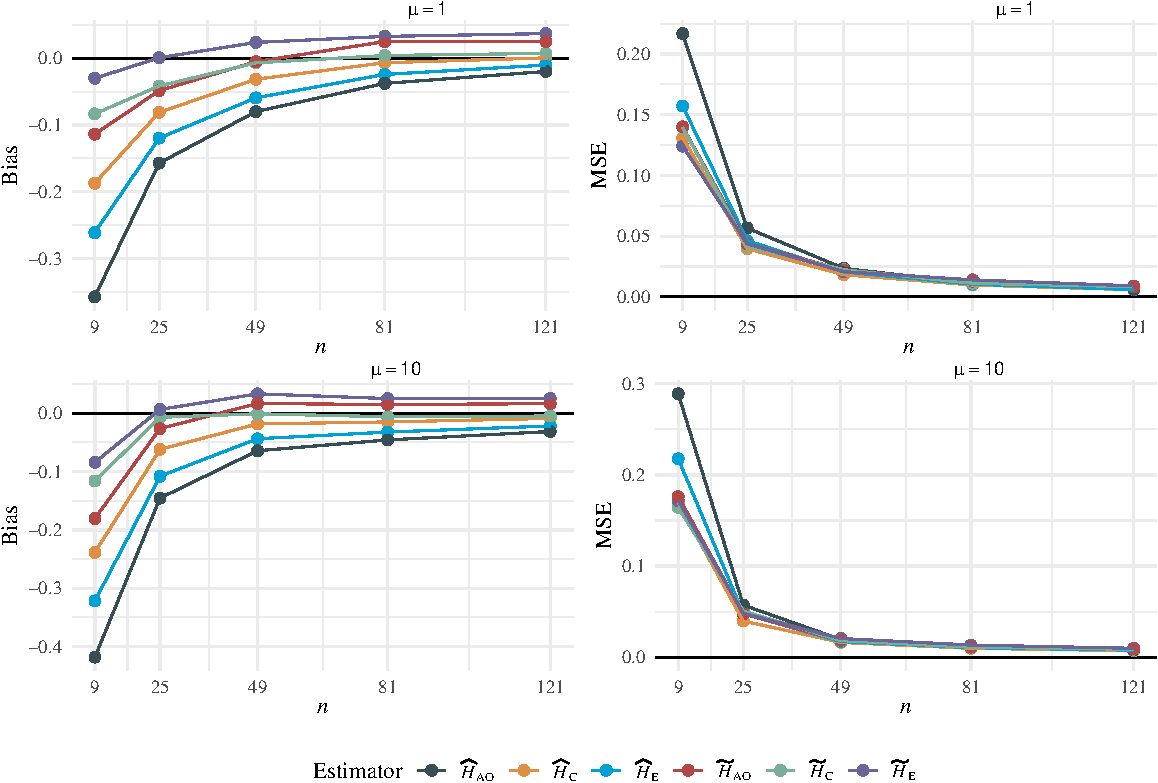
\includegraphics[width=0.95\linewidth]{Identifying-Heterogeneity-in-SAR-Data-with-New-Test-Statistics_files/figure-latex/Plot_bias_mse_gi0-1} %%%
\DIFdelendFL \DIFaddbeginFL 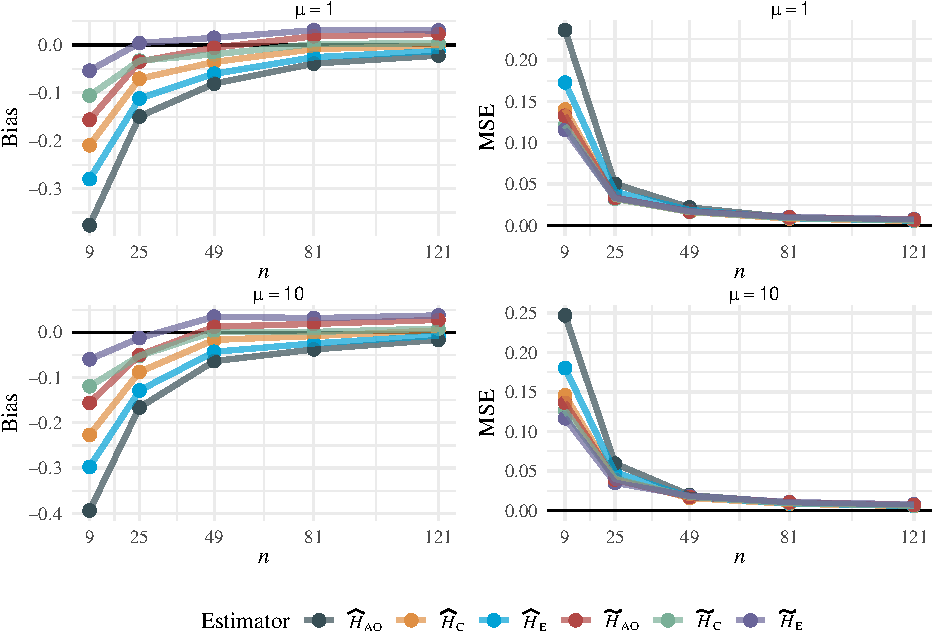
\includegraphics[width=0.95\linewidth]{R1-Identifying-Heterogeneity-in-SAR-Data-with-New-Test-Statistics_files/figure-latex/Plot_bias_mse_gi0-1} \DIFaddendFL \caption{Bias and MSE of the entropy estimators for the $\Gamma_{\text{SAR}}$, with $L=5$.}\label{fig:Plot_bias_mse_gi0}
\end{figure}

\setlength{\tabcolsep}{6pt}
\begin{table}[hbt]
\centering
\caption{\label{tab:table2}Bias and MSE of the entropy estimators for the $\Gamma_{\text{SAR}}$, with $L=5$.}
\resizebox{\ifdim\width>\linewidth\linewidth\else\width\fi}{!}{
\begin{tabular}[t]{crllllllllllll}
\toprule
\multicolumn{1}{c}{ } & \multicolumn{1}{c}{ } & \multicolumn{6}{c}{Bias} & \multicolumn{6}{c}{MSE} \\
\cmidrule(l{3pt}r{3pt}){3-8} \cmidrule(l{3pt}r{3pt}){9-14}
\multicolumn{1}{r}{$\bm{\mu}$} & \multicolumn{1}{r}{$\bm{n}$} & \multicolumn{1}{r}{$\bm{\widehat{H}_{\text{C}}}$} & \multicolumn{1}{r}{$\bm{\widehat{H}_{\text{E}}}$} & \multicolumn{1}{r}{$\bm{\widehat{H}_{\text{AO}}}$} & \multicolumn{1}{r}{$\bm{\widetilde{H}_{\text{C}}}$} & \multicolumn{1}{r}{$\bm{\widetilde{H}_{\text{E}}}$} & \multicolumn{1}{r}{$\bm{\widetilde{H}_{\text{AO}}}$} & \multicolumn{1}{r}{$\bm{\widehat{H}_{\text{C}}}$} & \multicolumn{1}{r}{$\bm{\widehat{H}_{\text{E}}}$} & \multicolumn{1}{r}{$\bm{\widehat{H}_{\text{AO}}}$} & \multicolumn{1}{r}{$\bm{\widetilde{H}_{\text{C}}}$} & \multicolumn{1}{r}{$\bm{\widetilde{H}_{\text{E}}}$} & \multicolumn{1}{r}{$\bm{\widetilde{H}_{\text{AO}}}$}\\
\midrule
 & $9$ & $-0.210$ & $-0.280$ & $-0.377$ & $-0.106$ & $-0.054$ & $-0.156$ & $\phantom{-}0.140$ & $\phantom{-}0.173$ & $\phantom{-}0.236$ & $\phantom{-}0.121$ & $\phantom{-}0.116$ & $\phantom{-}0.133$\\

 & $25$ & $-0.071$ & $-0.112$ & $-0.149$ & $-0.033$ & $\phantom{-}0.004$ & $-0.035$ & $\phantom{-}0.032$ & $\phantom{-}0.040$ & $\phantom{-}0.050$ & $\phantom{-}0.032$ & $\phantom{-}0.033$ & $\phantom{-}0.033$\\

 & $49$ & $-0.036$ & $-0.060$ & $-0.081$ & $-0.020$ & $\phantom{-}0.015$ & $-0.006$ & $\phantom{-}0.016$ & $\phantom{-}0.019$ & $\phantom{-}0.021$ & $\phantom{-}0.016$ & $\phantom{-}0.017$ & $\phantom{-}0.017$\\

 & $81$ & $-0.009$ & $-0.026$ & $-0.039$ & $\phantom{-}0.002$ & $\phantom{-}0.031$ & $\phantom{-}0.018$ & $\phantom{-}0.008$ & $\phantom{-}0.009$ & $\phantom{-}0.010$ & $\phantom{-}0.009$ & $\phantom{-}0.010$ & $\phantom{-}0.009$\\

\multirow{-5}{*}[2\dimexpr\aboverulesep+\belowrulesep+\cmidrulewidth]{\centering\arraybackslash 1} & $121$ & $-0.001$ & $-0.013$ & $-0.022$ & $\phantom{-}0.004$ & $\phantom{-}0.030$ & $\phantom{-}0.023$ & $\phantom{-}0.005$ & $\phantom{-}0.006$ & $\phantom{-}0.006$ & $\phantom{-}0.006$ & $\phantom{-}0.007$ & $\phantom{-}0.007$\\
\cmidrule{1-14}
 & $9$ & $-0.227$ & $-0.297$ & $-0.394$ & $-0.119$ & $-0.060$ & $-0.156$ & $\phantom{-}0.146$ & $\phantom{-}0.180$ & $\phantom{-}0.247$ & $\phantom{-}0.126$ & $\phantom{-}0.117$ & $\phantom{-}0.136$\\

 & $25$ & $-0.088$ & $-0.129$ & $-0.166$ & $-0.052$ & $-0.013$ & $-0.050$ & $\phantom{-}0.040$ & $\phantom{-}0.048$ & $\phantom{-}0.059$ & $\phantom{-}0.040$ & $\phantom{-}0.035$ & $\phantom{-}0.039$\\

 & $49$ & $-0.017$ & $-0.043$ & $-0.064$ & $\phantom{-}0.001$ & $\phantom{-}0.035$ & $\phantom{-}0.012$ & $\phantom{-}0.016$ & $\phantom{-}0.017$ & $\phantom{-}0.019$ & $\phantom{-}0.018$ & $\phantom{-}0.019$ & $\phantom{-}0.017$\\

 & $81$ & $-0.008$ & $-0.025$ & $-0.038$ & $\phantom{-}0.001$ & $\phantom{-}0.031$ & $\phantom{-}0.019$ & $\phantom{-}0.009$ & $\phantom{-}0.009$ & $\phantom{-}0.010$ & $\phantom{-}0.009$ & $\phantom{-}0.011$ & $\phantom{-}0.010$\\

\multirow{-5}{*}[2\dimexpr\aboverulesep+\belowrulesep+\cmidrulewidth]{\centering\arraybackslash 10} & $121$ & $\phantom{-}0.004$ & $-0.007$ & $-0.017$ & $\phantom{-}0.008$ & $\phantom{-}0.037$ & $\phantom{-}0.027$ & $\phantom{-}0.006$ & $\phantom{-}0.006$ & $\phantom{-}0.006$ & $\phantom{-}0.006$ & $\phantom{-}0.008$ & $\phantom{-}0.007$\\
\bottomrule
\end{tabular}}
\end{table}

\subsection{Coefficient of variation and a robust
alternative}\label{coefficient-of-variation-and-a-robust-alternative}

The population CV is defined as a ratio of the population standard
deviation \((\sigma)\) to the population mean \((\mu)\): \begin{align}
    \text{CV}=\frac{\sigma}{\mu}, \quad \mu \neq 0.
\end{align} The CV can be easily estimated as the ratio of the sample
mean to the sample standard deviation.

We explore a robust alternative to estimate the CV, as described
by~\cite{Ospina2019}: the ratio between the mean absolute deviation from
the median (MnAD) and the median, two well-known robust measures of
scale and location, respectively. The sample version for the MnAD is
defined as \(n^{-1}\sum_{i=1}^n|x_i-\widehat{Q}_2|\), where
\(\widehat{Q}_2\) is an estimate for the median of the population, for
example, the sample median.

\section{Hypothesis Testing}\label{sec:test}

We aim to test the following hypotheses: \[
\begin{cases}
  \mathcal{H}_0: \text{ The data come from the } \Gamma_{\text{SAR}}\text{ law},\\ 
  \mathcal{H}_1:\text{ The data come from the } G_I^0 \text{ distribution}.
\end{cases}
\] We are testing the hypothesis that the data are fully-developed
speckle versus the alternative of data with roughness. As for the
parametric problem, once it is not possible to define the hypothesis
\(\mathcal{H}_0=\alpha=-\infty\), it is impossible to solve this problem
with parametric inference alternatives (such as likelihood ratio, score,
gradient, and Wald hypothesis test). The proposed tests to solve this
physical problem in SAR systems are described below.

\subsection{The Proposed Test Based on Non-parametric
Entropy}\label{the-proposed-test-based-on-non-parametric-entropy}

For a random sample \(\bm{Z}=(Z_1, Z_2,\ldots,Z_n)\) from a distribution
\(\mathcal{D}\), a test statistic is proposed. It is based on an
empirical distribution that arises from the difference between
non-parametrically estimated entropies \(\widetilde{H}(\bm{Z})\) and the
analytical entropy of \(\Gamma_{\text{SAR}}\)~\eqref{E:E-gamma}
evaluated at the logarithm of the sample mean, where \(L\geq 1\) is
known.

Hence, the entropy-based test statistic is defined as: \begin{equation}
\label{Eq:test_e}
S(\bm{Z};L)= \widetilde{H}(\bm{Z})-\left[H_{\Gamma_{\text{SAR}}}(L)+\ln \overline{\bm{Z}}\right].
\end{equation}

This test statistic aims to assess the behavior of the data under the
null hypothesis using the empirical distribution. If the data represent
fully-developed speckle, the density should center around zero, i.e.,
\(S(\bm{Z};L)\approx 0\). Otherwise, the empirical distribution would
shift from zero under the alternative hypothesis, suggesting significant
differences and heterogeneous clutter.

The comparison between the bootstrap-improved estimators is shown in
Table~\ref{tab:table_time}, where the test accuracy under the null
hypothesis is presented alongside running times. The test accuracy is
evaluated through 1000 simulated samples of different sizes, with each
size replicated 100 times using bootstrap resampling.

The processing time is an important feature, especially considering the
application of these estimators to large datasets of SAR images, as seen
in Section~\ref{sec:Results}.

\begin{table}[H]
\centering\centering
\caption{\label{tab:table_time}Test accuracy and processing time for each bootstrap-improved estimator. }
\resizebox{\ifdim\width>\linewidth\linewidth\else\width\fi}{!}{
\begin{tabu} to \linewidth {>{\centering}X>{\centering}X>{\centering}X>{\centering}X>{\centering}X}
\toprule
\multicolumn{1}{c}{\textbf{Estimator}} & \multicolumn{1}{c}{$\bm{L}$} & \multicolumn{1}{c}{$\bm{n}$} & \multicolumn{1}{c}{$S(\bm{Z}; L)$} & \multicolumn{1}{c}{\textbf{ Time} (s)}\\
\midrule
 &  & $25$ & $-0.00152$ & 22.53\\

 &  & $49$ & $\phantom{-}0.00515$ & 40.35\\

 &  & $81$ & $\phantom{-}0.00625$ & 63.93\\

 & \multirow{-4}{*}[1.5\dimexpr\aboverulesep+\belowrulesep+\cmidrulewidth]{\centering\arraybackslash $2$} & $121$ & $\phantom{-}0.00751$ & 97.06\\

\cline{3-5}
 &  & $25$ & $-0.04332$ & 22.25\\

 &  & $49$ & $-0.01659$ & 33.42\\

 &  & $81$ & $-0.00393$ & 50.94\\

\multirow{-8}{*}[3.5\dimexpr\aboverulesep+\belowrulesep+\cmidrulewidth]{\centering\arraybackslash $\widetilde{H}_{\text{C}}$} & \multirow{-4}{*}[1.5\dimexpr\aboverulesep+\belowrulesep+\cmidrulewidth]{\centering\arraybackslash $8$} & $121$ & $\phantom{-}0.00261$ & 97.35\\
\cmidrule{1-5}
 &  & $25$ & $\phantom{-}0.02204$ & 4.66\\

 &  & $49$ & $\phantom{-}0.03452$ & 5.55\\

 &  & $81$ & $\phantom{-}0.03195$ & 6.89\\

 & \multirow{-4}{*}[1.5\dimexpr\aboverulesep+\belowrulesep+\cmidrulewidth]{\centering\arraybackslash $2$} & $121$ & $\phantom{-}0.03012$ & 7.90\\

\cline{3-5}
 &  & $25$ & $\phantom{-}0.00801$ & 4.81\\

 &  & $49$ & $\phantom{-}0.01654$ & 5.43\\

 &  & $81$ & $\phantom{-}0.03036$ & 6.38\\

\multirow{-8}{*}[3.5\dimexpr\aboverulesep+\belowrulesep+\cmidrulewidth]{\centering\arraybackslash $\widetilde{H}_{\text{E}}$} & \multirow{-4}{*}[1.5\dimexpr\aboverulesep+\belowrulesep+\cmidrulewidth]{\centering\arraybackslash $8$} & $121$ & $\phantom{-}0.03137$ & 7.46\\
\cmidrule{1-5}
 &  & $25$ & $-0.01935$ & 4.61\\

 &  & $49$ & $\phantom{-}0.00786$ & 5.19\\

 &  & $81$ & $\phantom{-}0.01995$ & 6.70\\

 & \multirow{-4}{*}[1.5\dimexpr\aboverulesep+\belowrulesep+\cmidrulewidth]{\centering\arraybackslash $2$} & $121$ & $\phantom{-}0.01741$ & 7.41\\

\cline{3-5}
 &  & $25$ & $-0.04020$ & 4.74\\

 &  & $49$ & $\phantom{-}0.00047$ & 5.35\\

 &  & $81$ & $\phantom{-}0.01176$ & 6.21\\

\multirow{-8}{*}[3.5\dimexpr\aboverulesep+\belowrulesep+\cmidrulewidth]{\centering\arraybackslash $\widetilde{H}_{\text{AO}}$} & \multirow{-4}{*}[1.5\dimexpr\aboverulesep+\belowrulesep+\cmidrulewidth]{\centering\arraybackslash $8$} & $121$ & $\phantom{-}0.02019$ & 7.48\\
\bottomrule
\end{tabu}}
\end{table}

As visible from Table~\ref{tab:table_time}, the accuracy of the test
results across the three estimators shows similarities in specific
sample sizes. However, practical scenarios in SAR image processing often
involve small sample sizes, typically obtained over windows of size
\(7\times7\).\\
It is also noteworthy that the \(\widetilde{H}_{\text{AO}}\) estimator
exhibited the shortest processing time, followed by
\(\widetilde{H}_{\text{E}}\) and \(\widetilde{H}_{\text{C}}\).
Considering this aspect, we select the \(\widetilde{H}_{\text{AO}}\)
estimator for subsequent simulations. Henceforth, the test statistical
~\eqref{Eq:test_e} will be denoted as:
\(S_{\widetilde{H}_{\text{AO}}}(\bm{Z}; L)\).

We now verify the normality of the data generated by the
\(S_{\widetilde{H}_{\text{AO}}}(\bm{Z}; L)\) test.
Figure~\ref{fig:Plot_density} shows the empirical densities obtained by
applying the \(S_{\widetilde{H}_{\text{AO}}}(\bm{Z}; L)\) test to
different sample sizes drawn from the \(\Gamma_{\text{SAR}}\)
distribution, where \(L\) takes values \(\left\{3,5, 8,11\right\}\) and
\(\mu=1\). Additionally, Table~\ref{tab:table_stat_combined} summarizes
the main descriptive statistics, including mean, standard
deviation~(SD), variance~(Var), skewness~(SK), excessive kurtosis~(EK)
and Anderson--Darling \(p\) values for normality. Results with \(p\)
values greater than \(0.05\) do not indicate a violation of the
normality assumption. A low variance, skewness, and excessive kurtosis
of almost zero indicate limited dispersion, asymmetry, and a light tail.
Normal Q--Q plots confirm no evidence against a normal distribution, as
shown in Figure~\ref{fig:Plot_normality_qq}.

\begin{figure}[hbt]
\DIFdelbeginFL %DIFDELCMD < 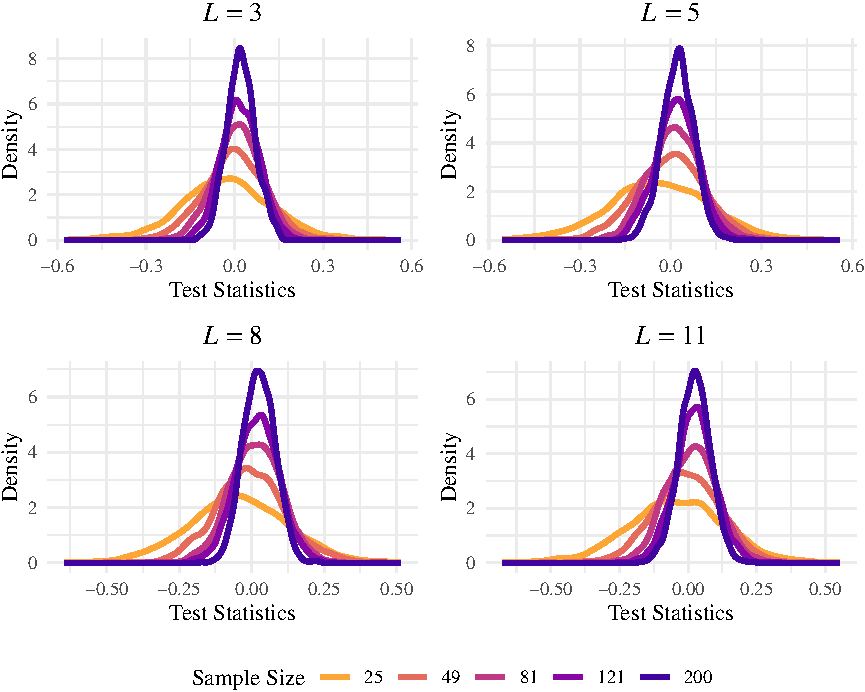
\includegraphics[width=0.95\linewidth]{Identifying-Heterogeneity-in-SAR-Data-with-New-Test-Statistics_files/figure-latex/Plot_density-1} %%%
\DIFdelendFL \DIFaddbeginFL 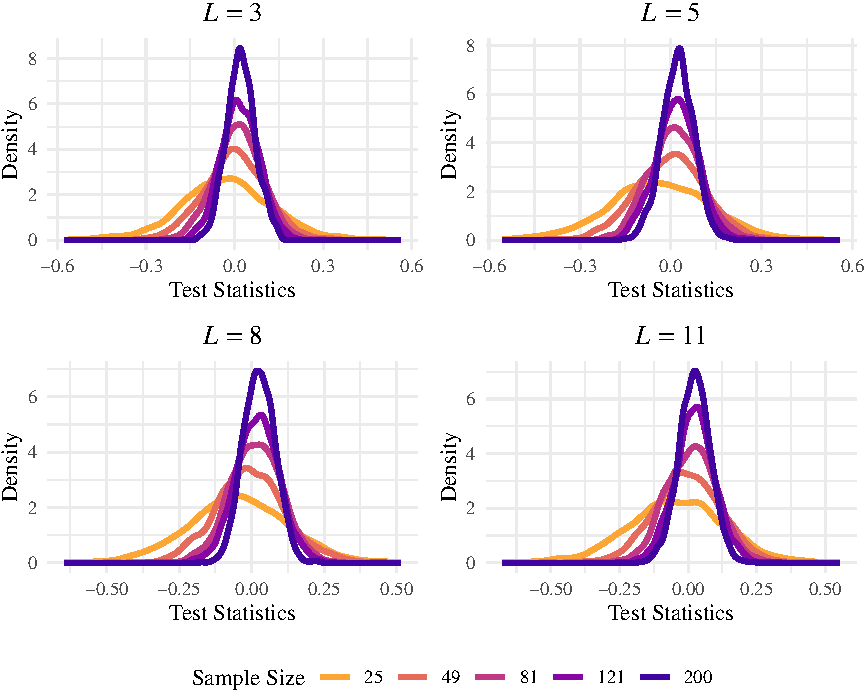
\includegraphics[width=0.95\linewidth]{R1-Identifying-Heterogeneity-in-SAR-Data-with-New-Test-Statistics_files/figure-latex/Plot_density-1} \DIFaddendFL \caption{Empirical densities obtained from $S_{\widetilde{H}_{\text{AO}}}(\bm{Z}; L)$ test under the null hypothesis.}\label{fig:Plot_density}
\end{figure}

\begin{table}[H]
\centering\centering\centering
\caption{\label{tab:table_stat_combined}Descriptive analysis of $S_{\widetilde{H}_{\text{AO}}}(\bm{Z}; L)$, with $L\in\left\{3,5, 8,11\right\}$ and $\mu=1$.}
\resizebox{\ifdim\width>\linewidth\linewidth\else\width\fi}{!}{
\begin{tabu} to \linewidth {>{\centering}X>{\centering}X>{\raggedleft}X>{\raggedleft}X>{\raggedleft}X>{\raggedleft}X>{\raggedleft}X>{\raggedleft}X}
\toprule
\multicolumn{1}{c}{$\bm{L}$} & \multicolumn{1}{c}{$\bm{n}$} & \multicolumn{1}{c}{\textbf{Mean}} & \multicolumn{1}{c}{\textbf{SD}} & \multicolumn{1}{c}{\textbf{Var}} & \multicolumn{1}{c}{\textbf{SK}} & \multicolumn{1}{c}{\textbf{EK}} & \multicolumn{1}{c}{$p$-\textbf{value}}\\
\midrule
 & $25$ & $-0.0280$ & $\phantom{-}0.1547$ & $\phantom{-}0.0239$ & $-0.0076$ & $\phantom{-}0.4734$ & $\phantom{-}0.0022$\\

 & $49$ & $-0.0003$ & $\phantom{-}0.1053$ & $\phantom{-}0.0111$ & $-0.0562$ & $\phantom{-}0.2610$ & $\phantom{-}0.0582$\\

 & $81$ & $\phantom{-}0.0124$ & $\phantom{-}0.0796$ & $\phantom{-}0.0063$ & $-0.0124$ & $\phantom{-}0.0536$ & $\phantom{-}0.5278$\\

 & $121$ & $\phantom{-}0.0187$ & $\phantom{-}0.0630$ & $\phantom{-}0.0040$ & $\phantom{-}0.0337$ & $-0.1826$ & $\phantom{-}0.5894$\\

\multirow{-5}{*}[2\dimexpr\aboverulesep+\belowrulesep+\cmidrulewidth]{\centering\arraybackslash 3} & $200$ & $\phantom{-}0.0215$ & $\phantom{-}0.0490$ & $\phantom{-}0.0024$ & $\phantom{-}0.0625$ & $-0.0473$ & $\phantom{-}0.0860$\\
\cmidrule{1-8}
 & $25$ & $-0.0379$ & $\phantom{-}0.1669$ & $\phantom{-}0.0278$ & $\phantom{-}0.0007$ & $\phantom{-}0.1420$ & $\phantom{-}0.3267$\\

 & $49$ & $-0.0015$ & $\phantom{-}0.1150$ & $\phantom{-}0.0132$ & $-0.1025$ & $\phantom{-}0.1998$ & $\phantom{-}0.2582$\\

 & $81$ & $\phantom{-}0.0145$ & $\phantom{-}0.0869$ & $\phantom{-}0.0075$ & $\phantom{-}0.1008$ & $\phantom{-}0.5297$ & $\phantom{-}0.1121$\\

 & $121$ & $\phantom{-}0.0198$ & $\phantom{-}0.0687$ & $\phantom{-}0.0047$ & $\phantom{-}0.0127$ & $\phantom{-}0.0222$ & $\phantom{-}0.2919$\\

\multirow{-5}{*}[2\dimexpr\aboverulesep+\belowrulesep+\cmidrulewidth]{\centering\arraybackslash 5} & $200$ & $\phantom{-}0.0236$ & $\phantom{-}0.0529$ & $\phantom{-}0.0028$ & $-0.0467$ & $\phantom{-}0.0977$ & $\phantom{-}0.3346$\\
\cmidrule{1-8}
 & $25$ & $-0.0464$ & $\phantom{-}0.1680$ & $\phantom{-}0.0282$ & $-0.0121$ & $\phantom{-}0.0980$ & $\phantom{-}0.6477$\\

 & $49$ & $-0.0031$ & $\phantom{-}0.1202$ & $\phantom{-}0.0144$ & $\phantom{-}0.1282$ & $\phantom{-}0.2000$ & $\phantom{-}0.0038$\\

 & $81$ & $\phantom{-}0.0137$ & $\phantom{-}0.0883$ & $\phantom{-}0.0078$ & $-0.0279$ & $\phantom{-}0.2554$ & $\phantom{-}0.5567$\\

 & $121$ & $\phantom{-}0.0200$ & $\phantom{-}0.0738$ & $\phantom{-}0.0055$ & $-0.0089$ & $\phantom{-}0.0686$ & $\phantom{-}0.7502$\\

\multirow{-5}{*}[2\dimexpr\aboverulesep+\belowrulesep+\cmidrulewidth]{\centering\arraybackslash 8} & $200$ & $\phantom{-}0.0260$ & $\phantom{-}0.0546$ & $\phantom{-}0.0030$ & $\phantom{-}0.0716$ & $-0.0349$ & $\phantom{-}0.3771$\\
\cmidrule{1-8}
 & $25$ & $-0.0442$ & $\phantom{-}0.1735$ & $\phantom{-}0.0301$ & $-0.1422$ & $\phantom{-}0.2413$ & $\phantom{-}0.0981$\\

 & $49$ & $-0.0019$ & $\phantom{-}0.1201$ & $\phantom{-}0.0144$ & $-0.0503$ & $\phantom{-}0.1464$ & $\phantom{-}0.9576$\\

 & $81$ & $\phantom{-}0.0127$ & $\phantom{-}0.0917$ & $\phantom{-}0.0084$ & $-0.0172$ & $\phantom{-}0.0333$ & $\phantom{-}0.3179$\\

 & $121$ & $\phantom{-}0.0239$ & $\phantom{-}0.0729$ & $\phantom{-}0.0053$ & $-0.0127$ & $\phantom{-}0.2102$ & $\phantom{-}0.0596$\\

\multirow{-5}{*}[2\dimexpr\aboverulesep+\belowrulesep+\cmidrulewidth]{\centering\arraybackslash 11} & $200$ & $\phantom{-}0.0234$ & $\phantom{-}0.0572$ & $\phantom{-}0.0033$ & $-0.0233$ & $\phantom{-}0.1072$ & $\phantom{-}0.6740$\\
\bottomrule
\end{tabu}}
\end{table}

\begin{figure}[H]
\DIFdelbeginFL %DIFDELCMD < 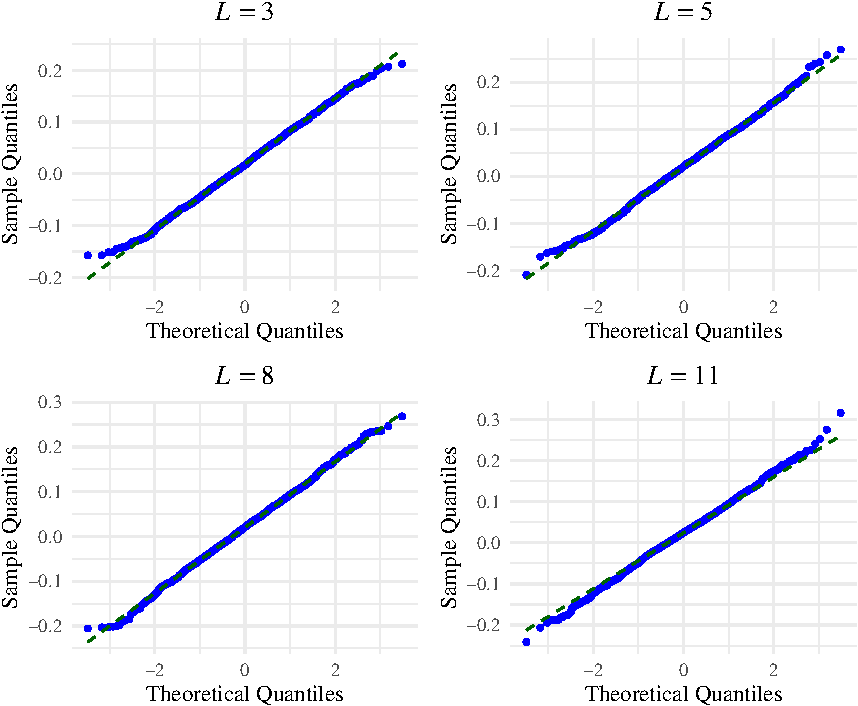
\includegraphics[width=0.9\linewidth]{Identifying-Heterogeneity-in-SAR-Data-with-New-Test-Statistics_files/figure-latex/Plot_normality_qq-1} %%%
\DIFdelendFL \DIFaddbeginFL 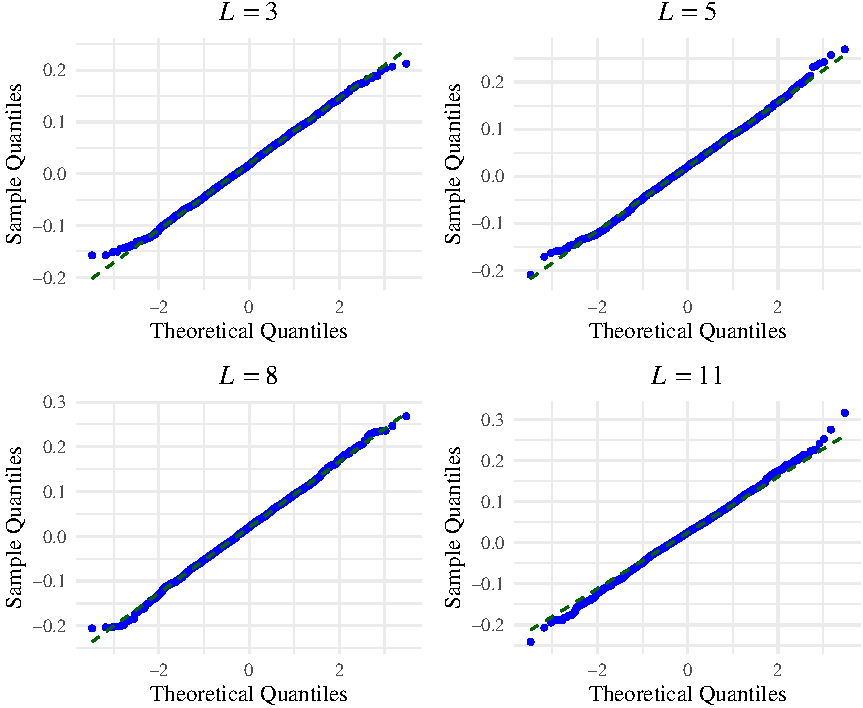
\includegraphics[width=0.9\linewidth]{R1-Identifying-Heterogeneity-in-SAR-Data-with-New-Test-Statistics_files/figure-latex/Plot_normality_qq-1} \DIFaddendFL \caption{Normal Q--Q plots for  $n=121$. \DIFaddbeginFL \DIFaddFL{The dashed green lines in the Q--Q plots represent theoretical expected quantiles for a normal distribution. Variations in the scales of the axes reflect differences in the range of values across datasets.}\DIFaddendFL }\label{fig:Plot_normality_qq}
\end{figure}

After checking the data's normality, we examined the proposed test's
abilities in terms of size \DIFdelbegin \DIFdel{and power. }\DIFdelend \DIFaddbegin \DIFadd{(Type I error rate) and power (probability of
correctly rejecting the null hypothesis when the alternative hypothesis
is true).
}

\DIFaddend Under \(\mathcal{H}_0\), the distribution of the test statistic is
asymptotically normal. Therefore, the \(p\) values are calculated as
\(2\Phi(-|\varepsilon|)\), where \(\Phi\) is the standard Gaussian
cumulative distribution function, and \(\varepsilon\) is the
standardized test statistic given by: \[
\varepsilon=\frac{\widetilde{H}_{\text{AO}}(\bm{Z})-\left[H_{\Gamma_{\text{SAR}}}(L)+\ln \overline{\bm{Z}}\right]}{\widehat\sigma}.
\]

We \DIFdelbegin \DIFdel{have nominal }\DIFdelend \DIFaddbegin \DIFadd{conducted the test at nominal significance }\DIFaddend levels of
\SI{1}{\percent}, \SI{5}{\percent}, and \SI{10}{\percent}. \DIFdelbegin \DIFdel{In terms of size, }\DIFdelend \DIFaddbegin \DIFadd{These levels
represent the probability of rejecting the null hypothesis when it is
actually true (Type I error rates). To verify that the test maintains
these nominal levels, we performed }\DIFaddend \(1000\) simulations \DIFdelbegin \DIFdel{were used for
different sample sizes from the }\DIFdelend \DIFaddbegin \DIFadd{under the null
hypothesis (}\DIFaddend \(\Gamma_{\text{SAR}}\) distribution\DIFdelbegin \DIFdel{,
with varying }\DIFdelend \DIFaddbegin \DIFadd{), with different sample
sizes and }\DIFaddend values of \(L\), and \(\mu=1\). In all cases, the \DIFdelbegin \DIFdel{nominal
level was achieved.
We assessed the testpower using }\DIFdelend \DIFaddbegin \DIFadd{observed
Type I error rates were consistent with the nominal levels, indicating
that the test maintains the specified significance levels.
}

\DIFadd{We also evaluated the test's power by performing }\DIFaddend \(1000\) simulations
\DIFdelbegin \DIFdel{for different sample sizes from the }\DIFdelend \DIFaddbegin \DIFadd{under the alternative hypothesis (}\DIFaddend \(G_I^0\) distribution\DIFdelbegin \DIFdel{,
}\DIFdelend \DIFaddbegin \DIFadd{) }\DIFaddend with \(\mu=1\)
\DIFdelbegin \DIFdel{, }\DIFdelend and \(\alpha=-2\). The power generally improves with increasing sample
size and number of looks. The results are shown in
Table~\ref{tab:table_size_power}.

\begin{table}[htb]
\centering\centering
\caption{\label{tab:table_size_power}Size and Power of the $S_{\widetilde{H}_{\text{AO}}}(\bm{Z})$ test statistic.}
\resizebox{\ifdim\width>\linewidth\linewidth\else\width\fi}{!}{
\begin{tabu} to \linewidth {>{\centering}X>{\centering}X>{\centering}X>{\centering}X>{\centering}X>{\centering}X>{\centering}X>{\centering}X}
\toprule
\multicolumn{1}{c}{ } & \multicolumn{1}{c}{ } & \multicolumn{3}{c}{Size} & \multicolumn{3}{c}{Power} \\
\cmidrule(l{3pt}r{3pt}){3-5} \cmidrule(l{3pt}r{3pt}){6-8}
\multicolumn{1}{c}{$\bm{L}$} & \multicolumn{1}{c}{$\bm{n}$} & \multicolumn{1}{c}{$\bm{1\%}$} & \multicolumn{1}{c}{$\bm{5\%}$} & \multicolumn{1}{c}{$\bm{10\%}$} & \multicolumn{1}{c}{$\bm{1\%}$} & \multicolumn{1}{c}{$\bm{5\%}$} & \multicolumn{1}{c}{$\bm{10\%}$}\\
\midrule
 & 25 & $\phantom{-}0.0160$ & $\phantom{-}0.0620$ & $\phantom{-}0.1070$ & $\phantom{-}0.6900$ & $\phantom{-}0.8450$ & $\phantom{-}0.8340$\\

 & 49 & $\phantom{-}0.0100$ & $\phantom{-}0.0480$ & $\phantom{-}0.0960$ & $\phantom{-}0.6890$ & $\phantom{-}0.8920$ & $\phantom{-}0.8480$\\

 & 81 & $\phantom{-}0.0120$ & $\phantom{-}0.0490$ & $\phantom{-}0.1080$ & $\phantom{-}0.6260$ & $\phantom{-}0.8750$ & $\phantom{-}0.8540$\\

\multirow{-4}{*}[1.5\dimexpr\aboverulesep+\belowrulesep+\cmidrulewidth]{\centering\arraybackslash 3} & 121 & $\phantom{-}0.0090$ & $\phantom{-}0.0690$ & $\phantom{-}0.1190$ & $\phantom{-}0.5680$ & $\phantom{-}0.8620$ & $\phantom{-}0.8230$\\
\cmidrule{1-8}
 & 25 & $\phantom{-}0.0210$ & $\phantom{-}0.0660$ & $\phantom{-}0.1130$ & $\phantom{-}0.9120$ & $\phantom{-}0.9620$ & $\phantom{-}0.9880$\\

 & 49 & $\phantom{-}0.0100$ & $\phantom{-}0.0460$ & $\phantom{-}0.1080$ & $\phantom{-}0.9470$ & $\phantom{-}0.9820$ & $\phantom{-}0.9960$\\

 & 81 & $\phantom{-}0.0120$ & $\phantom{-}0.0560$ & $\phantom{-}0.1070$ & $\phantom{-}0.9580$ & $\phantom{-}0.9900$ & $\phantom{-}0.9960$\\

\multirow{-4}{*}[1.5\dimexpr\aboverulesep+\belowrulesep+\cmidrulewidth]{\centering\arraybackslash 5} & 121 & $\phantom{-}0.0150$ & $\phantom{-}0.0640$ & $\phantom{-}0.1150$ & $\phantom{-}0.9420$ & $\phantom{-}0.9780$ & $\phantom{-}0.9950$\\
\cmidrule{1-8}
 & 25 & $\phantom{-}0.0210$ & $\phantom{-}0.0650$ & $\phantom{-}0.1080$ & $\phantom{-}0.9930$ & $\phantom{-}0.9950$ & $\phantom{-}0.9970$\\

 & 49 & $\phantom{-}0.0060$ & $\phantom{-}0.0470$ & $\phantom{-}0.0860$ & $\phantom{-}0.9980$ & $\phantom{-}1.0000$ & $\phantom{-}0.9970$\\

 & 81 & $\phantom{-}0.0120$ & $\phantom{-}0.0490$ & $\phantom{-}0.1000$ & $\phantom{-}0.9930$ & $\phantom{-}0.9980$ & $\phantom{-}0.9990$\\

\multirow{-4}{*}[1.5\dimexpr\aboverulesep+\belowrulesep+\cmidrulewidth]{\centering\arraybackslash 8} & 121 & $\phantom{-}0.0150$ & $\phantom{-}0.0650$ & $\phantom{-}0.1220$ & $\phantom{-}0.9970$ & $\phantom{-}0.9990$ & $\phantom{-}0.9980$\\
\cmidrule{1-8}
 & 25 & $\phantom{-}0.0130$ & $\phantom{-}0.0610$ & $\phantom{-}0.1000$ & $\phantom{-}0.9990$ & $\phantom{-}0.9990$ & $\phantom{-}0.9990$\\

 & 49 & $\phantom{-}0.0100$ & $\phantom{-}0.0450$ & $\phantom{-}0.0920$ & $\phantom{-}0.9980$ & $\phantom{-}0.9990$ & $\phantom{-}0.9990$\\

 & 81 & $\phantom{-}0.0170$ & $\phantom{-}0.0530$ & $\phantom{-}0.1050$ & $\phantom{-}1.0000$ & $\phantom{-}1.0000$ & $\phantom{-}1.0000$\\

\multirow{-4}{*}[1.5\dimexpr\aboverulesep+\belowrulesep+\cmidrulewidth]{\centering\arraybackslash 11} & 121 & $\phantom{-}0.0160$ & $\phantom{-}0.0680$ & $\phantom{-}0.1180$ & $\phantom{-}0.9980$ & $\phantom{-}1.0000$ & $\phantom{-}0.9980$\\
\bottomrule
\end{tabu}}
\end{table}

\subsection{The Proposed Test Based on Coefficient of Variation and a
Robust
Alternative}\label{the-proposed-test-based-on-coefficient-of-variation-and-a-robust-alternative}

In addition to the \(S_{\widetilde{H}_{\text{AO}}}(\bm{Z}; L)\) test, we
also propose a test statistic based on the classical CV. This test
statistic is defined as follows: \begin{align}
    T_{\text{CV}}=\frac{S}{\overline{Z}},
\end{align} where \(S\) and \(\overline{Z}\) are the sample standard
deviation and mean, respectively.

Similarly, we use another test statistic based on the ratio of the MnAD
to the median. This statistic is given by: \begin{align}
    T_{\text{CV}_{\text{MnAD}}}=\frac{\text{MnAD}}{\text{Median}}.
\end{align}

We proceed to identify suitable models for these estimators of the CV,
and then form test statistics.

The situations in which the use of CV and \(\text{CV}_{\text{MnAD}}\)
may be appropriate, i.e., when the observations are positive, the
log-normal (LN) and the inverse Gaussian distribution (IG) are often
more appropriate than the Gamma and Weibull
distributions~\cite{Chaubey2017,takagi1997application}.

It is shown that the IG distribution is well approximated by the
log-normal distribution, which means that the IG distribution also does
not share the problem of the non-existence of a fixed-width confidence
interval with the Gaussian case~\cite{whitmore1978}.

The biparametric LN distribution has density:

\begin{align}
    f_Z(z;\mu_{\text{LN}}, \sigma_{\text{LN}} )=\frac{1}{\sigma_{\text{LN}} z\sqrt{2\pi}}\exp\left\{-\frac{(\ln z- \mu_{\text{LN}})^2}{2\sigma_{\text{LN}}^2}\right\}\mathbbm 1_{\mathbbm R_+}(z),
\end{align}\\
with \(\mu_{\text{LN}}\) is any real number, and \(\sigma_{\text{LN}}\)
is positive.

\subsection{Model Selection Criterion}\label{model-selection-criterion}

We used the Akaike information criterion (AIC) and the Bayesian
information criterion (BIC) to select the best-fitting distribution.

The AIC deals with the trade-off between the goodness-of-fit and the
model's simplicity in terms of the number of model
parameters~\cite{Burnham2004}. The model or distribution with the lowest
value of AIC is chosen to be the best. The BIC assesses goodness-of-fit
of a distribution or model, but avoids overfitting by penalising
additional degrees of freedom~\cite{Dziak2019}. The model with the
lowest BIC value is chosen as the best.

The AIC and BIC results in
Tables~\ref{tab:table_aic_gamma}--\ref{tab:table_aic_gio_MnADmedian}
indicate that the CV and \(\text{CV}_{\text{MnAD}}\) data from different
distributed \(\Gamma_{\text{SAR}}\) and \(G_I^0\) synthetic sample sizes
match the properties of an LN distribution. It is important to note that
this conclusion was drawn empirically based on a dictionary of
analytically tractable distributions and well-defined under
biparametric, unimodal, asymmetric, and positive distributions.

Figures~\ref{fig:Plot_cv}--\ref{fig:Plot_madmed_gi0_MnADmedian} show
empirical and fitted density plots, Q--Q plots, P--P plots, as well as
empirical and fitted cumulative distribution functions. They provide
qualitative sources that confirm that the LN distribution is the most
appropriate distribution. As expected, both test statistics work well
under the null hypothesis. Under the alternative hypothesis, the P--P
plot shows that \(\text{CV}_{\text{MnAD}}\) is more robust than CV,
although both statistics suffer from the tail effect caused by the
distributed \(G_I^0\) data.

\begin{table}[H]
\centering\centering
\caption{\label{tab:table_aic_gamma}AIC and BIC values for evaluating the best distribution with CV data from $\Gamma_{\text{SAR}}$.}
\resizebox{\ifdim\width>\linewidth\linewidth\else\width\fi}{!}{
\begin{tabu} to \linewidth {>{\centering}X>{\centering}X>{\centering}X>{\centering}X>{\raggedleft}X>{\raggedleft}X>{\raggedleft}X}
\toprule
\multicolumn{1}{c}{\textbf{Criterion}} & \multicolumn{1}{c}{$\bm{n}$} & \multicolumn{1}{c}{\textbf{Normal}} & \multicolumn{1}{c}{\textbf{Lognormal}} & \multicolumn{1}{c}{\textbf{Gamma}} & \multicolumn{1}{c}{\textbf{Weibull}} & \multicolumn{1}{c}{\textbf{Inverse Gaussian}}\\
\midrule
 & $25$ & $-38031.9$ & $-38266.7$ & $-38311.8$ & $-36413.2$ & $-38261.6$\\

 & $49$ & $-47698.2$ & $-47913.7$ & $-47905.6$ & $-45554.0$ & $-47911.6$\\

 & $81$ & $-55382.1$ & $-55494.7$ & $-55494.9$ & $-53220.4$ & $-55493.8$\\

\multirow{-4}{*}[1.5\dimexpr\aboverulesep+\belowrulesep+\cmidrulewidth]{\centering\arraybackslash AIC} & $121$ & $-61344.9$ & $-61470.8$ & $-61453.8$ & $-58876.0$ & $-61470.5$\\
\cmidrule{1-7}
 & $25$ & $-38016.7$ & $-38251.5$ & $-38296.6$ & $-36398.0$ & $-38246.4$\\

 & $49$ & $-47683.0$ & $-47898.5$ & $-47890.4$ & $-45538.7$ & $-47896.4$\\

 & $81$ & $-55366.9$ & $-55479.5$ & $-55479.6$ & $-53205.2$ & $-55478.6$\\

\multirow{-4}{*}[1.5\dimexpr\aboverulesep+\belowrulesep+\cmidrulewidth]{\centering\arraybackslash BIC} & $121$ & $-61329.7$ & $-61455.6$ & $-61438.6$ & $-58860.8$ & $-61455.2$\\
\bottomrule
\end{tabu}}
\end{table}

\begin{table}[H]
\centering\centering
\caption{\label{tab:table_aic}AIC and BIC values for evaluating the best distribution with CV data from $G_I^0$.}
\resizebox{\ifdim\width>\linewidth\linewidth\else\width\fi}{!}{
\begin{tabu} to \linewidth {>{\centering}X>{\centering}X>{\centering}X>{\centering}X>{\centering}X>{\centering}X>{\centering}X}
\toprule
\multicolumn{1}{c}{\textbf{Criterion}} & \multicolumn{1}{c}{$\bm{n}$} & \multicolumn{1}{c}{\textbf{Normal}} & \multicolumn{1}{c}{\textbf{Lognormal}} & \multicolumn{1}{c}{\textbf{Gamma}} & \multicolumn{1}{c}{\textbf{Weibull}} & \multicolumn{1}{c}{\textbf{Inverse Gaussian}}\\
\midrule
 & $25$ & $\phantom{-}8254.04$ & $\phantom{-}2186.31$ & $\phantom{-}3628.40$ & $\phantom{-}8383.58$ & $\phantom{-}2257.63$\\

 & $49$ & $\phantom{-}8821.79$ & $\phantom{-}1689.03$ & $\phantom{-}3483.10$ & $\phantom{-}9533.53$ & $\phantom{-}1835.29$\\

 & $81$ & $\phantom{-}8525.81$ & $\phantom{-}866.29$ & $\phantom{-}2853.31$ & $\phantom{-}9822.48$ & $\phantom{-}1057.91$\\

\multirow{-4}{*}[1.5\dimexpr\aboverulesep+\belowrulesep+\cmidrulewidth]{\centering\arraybackslash AIC} & $121$ & $\phantom{-}8708.81$ & $\phantom{-}131.86$ & $\phantom{-}2341.06$ & $\phantom{-}10506.49$ & $\phantom{-}398.53$\\
\cmidrule{1-7}
 & $25$ & $\phantom{-}8269.27$ & $\phantom{-}2201.54$ & $\phantom{-}3643.63$ & $\phantom{-}8398.81$ & $\phantom{-}2272.86$\\

 & $49$ & $\phantom{-}8837.02$ & $\phantom{-}1704.26$ & $\phantom{-}3498.33$ & $\phantom{-}9548.76$ & $\phantom{-}1850.52$\\

 & $81$ & $\phantom{-}8541.04$ & $\phantom{-}881.52$ & $\phantom{-}2868.55$ & $\phantom{-}9837.72$ & $\phantom{-}1073.14$\\

\multirow{-4}{*}[1.5\dimexpr\aboverulesep+\belowrulesep+\cmidrulewidth]{\centering\arraybackslash BIC} & $121$ & $\phantom{-}8724.04$ & $\phantom{-}147.09$ & $\phantom{-}2356.29$ & $\phantom{-}10521.72$ & $\phantom{-}413.76$\\
\bottomrule
\end{tabu}}
\end{table}

\begin{table}[H]
\centering\centering
\caption{\label{tab:table_aic_gamma_madmed}AIC and BIC values for evaluating the best distribution with $\text{CV}_{\text{MnAD}}$ data from $\Gamma_{\text{SAR}}$.}
\resizebox{\ifdim\width>\linewidth\linewidth\else\width\fi}{!}{
\begin{tabu} to \linewidth {>{\centering}X>{\centering}X>{\centering}X>{\centering}X>{\centering}X>{\centering}X>{\centering}X}
\toprule
\multicolumn{1}{c}{\textbf{Criterion}} & \multicolumn{1}{c}{$\bm{n}$} & \multicolumn{1}{c}{\textbf{Normal}} & \multicolumn{1}{c}{\textbf{Lognormal}} & \multicolumn{1}{c}{\textbf{Gamma}} & \multicolumn{1}{c}{\textbf{Weibull}} & \multicolumn{1}{c}{\textbf{Inverse Gaussian}}\\
\midrule
 & $25$ & $-38375.56$ & $-39147.85$ & $-39066.29$ & $-36652.49$ & $-39143.61$\\

 & $49$ & $-48386.11$ & $-48795.32$ & $-48745.48$ & $-46240.91$ & $-48793.83$\\

 & $81$ & $-56072.87$ & $-56322.32$ & $-56290.02$ & $-53836.04$ & $-56322.12$\\

\multirow{-4}{*}[1.5\dimexpr\aboverulesep+\belowrulesep+\cmidrulewidth]{\centering\arraybackslash AIC} & $121$ & $-62217.14$ & $-62394.77$ & $-62369.32$ & $-59861.80$ & $-62394.57$\\
\cmidrule{1-7}
 & $25$ & $-38360.32$ & $-39132.62$ & $-39051.05$ & $-36637.26$ & $-39128.38$\\

 & $49$ & $-48370.87$ & $-48780.09$ & $-48730.25$ & $-46225.67$ & $-48778.60$\\

 & $81$ & $-56057.64$ & $-56307.09$ & $-56274.79$ & $-53820.81$ & $-56306.89$\\

\multirow{-4}{*}[1.5\dimexpr\aboverulesep+\belowrulesep+\cmidrulewidth]{\centering\arraybackslash BIC} & $121$ & $-62201.91$ & $-62379.54$ & $-62354.09$ & $-59846.56$ & $-62379.33$\\
\bottomrule
\end{tabu}}
\end{table}

\begin{table}[H]
\centering\centering
\caption{\label{tab:table_aic_gio_MnADmedian}AIC and BIC values for evaluating the best distribution with $\text{CV}_{\text{MnAD}}$ data from $G_I^0$.}
\resizebox{\ifdim\width>\linewidth\linewidth\else\width\fi}{!}{
\begin{tabu} to \linewidth {>{\centering}X>{\centering}X>{\centering}X>{\centering}X>{\centering}X>{\centering}X>{\centering}X}
\toprule
\multicolumn{1}{c}{\textbf{Criterion}} & \multicolumn{1}{c}{$\bm{n}$} & \multicolumn{1}{c}{\textbf{Normal}} & \multicolumn{1}{c}{\textbf{Lognormal}} & \multicolumn{1}{c}{\textbf{Gamma}} & \multicolumn{1}{c}{\textbf{Weibull}} & \multicolumn{1}{c}{\textbf{Inverse Gaussian}}\\
\midrule
 & $25$ & $-13302.39$ & $-15575.23$ & $-15158.42$ & $-11933.35$ & $-15565.03$\\

 & $49$ & $-23265.27$ & $-24529.72$ & $-24284.47$ & $-20986.94$ & $-24522.28$\\

 & $81$ & $-29908.19$ & $-30960.38$ & $-30747.90$ & $-25233.41$ & $-30946.54$\\

\multirow{-4}{*}[1.5\dimexpr\aboverulesep+\belowrulesep+\cmidrulewidth]{\centering\arraybackslash AIC} & $121$ & $-36496.78$ & $-37128.07$ & $-36991.41$ & $-32366.52$ & $-37123.20$\\
\cmidrule{1-7}
 & $25$ & $-13287.16$ & $-15559.99$ & $-15143.19$ & $-11918.12$ & $-15549.80$\\

 & $49$ & $-23250.04$ & $-24514.48$ & $-24269.24$ & $-20971.71$ & $-24507.05$\\

 & $81$ & $-29892.96$ & $-30945.15$ & $-30732.67$ & $-25218.17$ & $-30931.31$\\

\multirow{-4}{*}[1.5\dimexpr\aboverulesep+\belowrulesep+\cmidrulewidth]{\centering\arraybackslash BIC} & $121$ & $-36481.55$ & $-37112.84$ & $-36976.18$ & $-32351.28$ & $-37107.97$\\
\bottomrule
\end{tabu}}
\end{table}

\begin{figure}[H]

{\centering \DIFdelbeginFL %DIFDELCMD < 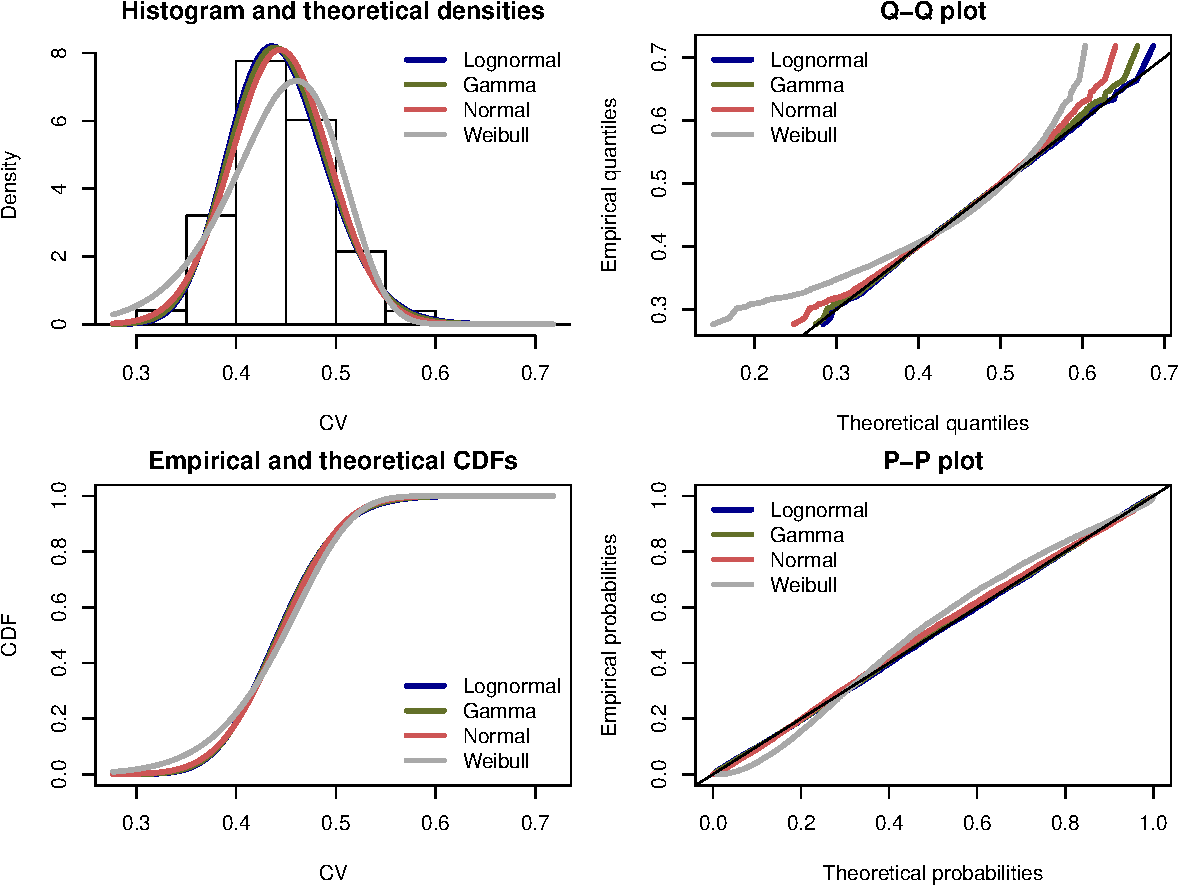
\includegraphics[width=1\linewidth]{Identifying-Heterogeneity-in-SAR-Data-with-New-Test-Statistics_files/figure-latex/Plot_cv_gamma-1} 
%DIFDELCMD < %%%
\DIFdelendFL \DIFaddbeginFL 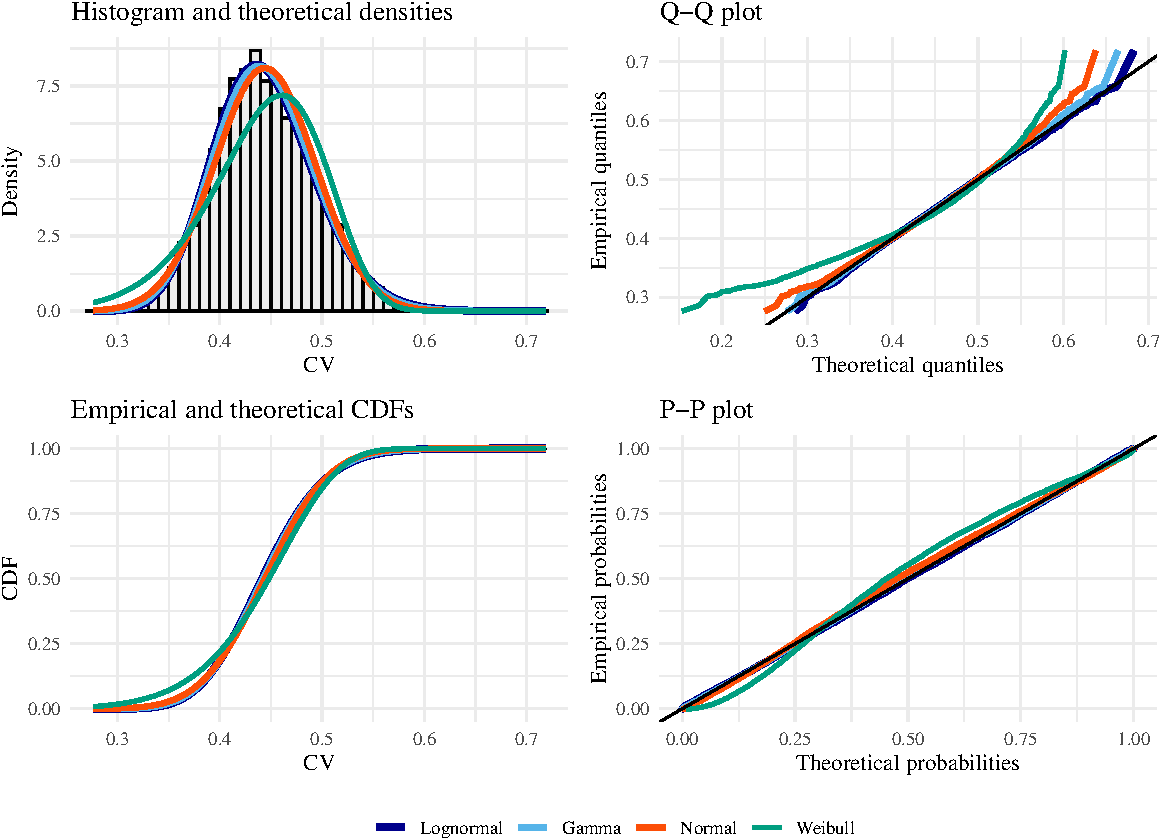
\includegraphics[width=1\linewidth]{R1-Identifying-Heterogeneity-in-SAR-Data-with-New-Test-Statistics_files/figure-latex/Plot_cv_gamma-1} 
\DIFaddendFL 

}

\caption{Goodness of fit plots for evaluating the best distribution with CV data from $\Gamma_{\text{SAR}}$ (under the null hypothesis), with $n=49$, $L=5$, and $\mu=1$.}\label{fig:Plot_cv_gamma}
\end{figure}

\begin{figure}[H]

{\centering \DIFdelbeginFL %DIFDELCMD < 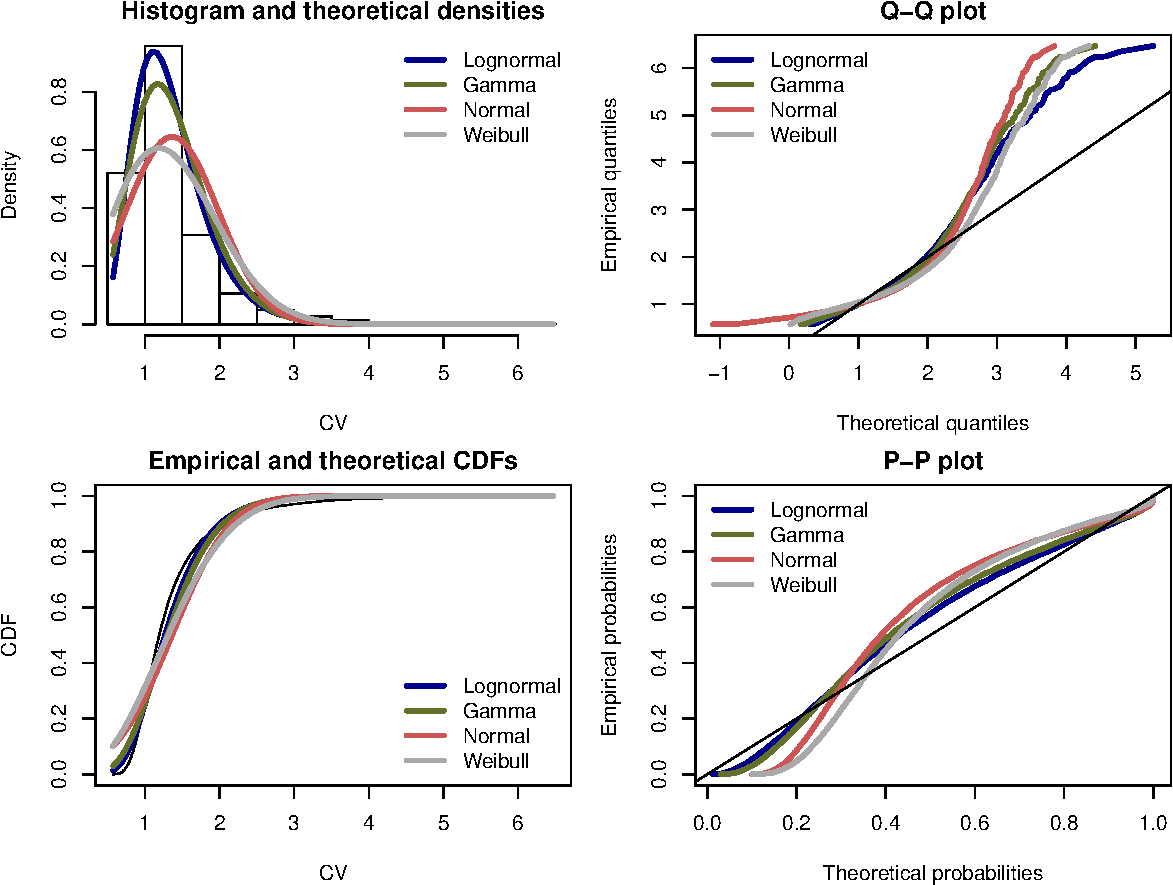
\includegraphics[width=1\linewidth]{Identifying-Heterogeneity-in-SAR-Data-with-New-Test-Statistics_files/figure-latex/Plot_cv-1} 
%DIFDELCMD < %%%
\DIFdelendFL \DIFaddbeginFL 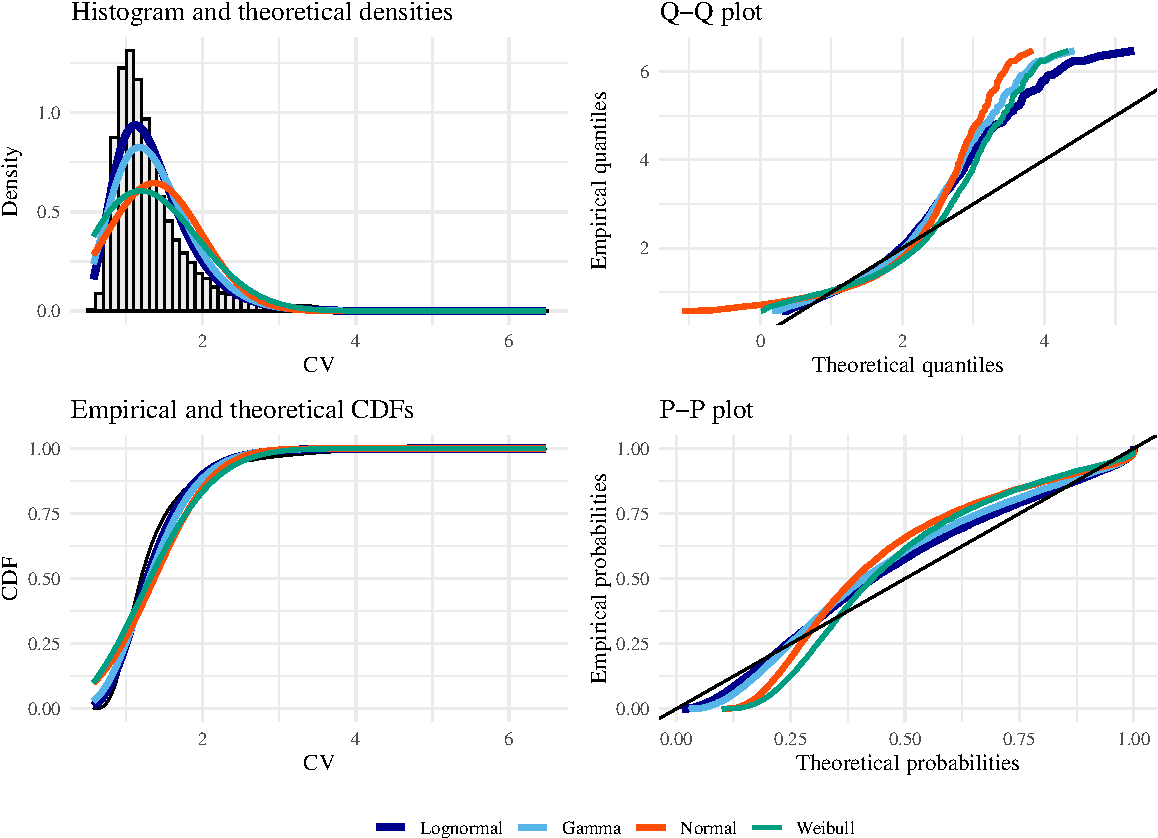
\includegraphics[width=1\linewidth]{R1-Identifying-Heterogeneity-in-SAR-Data-with-New-Test-Statistics_files/figure-latex/Plot_cv-1} 
\DIFaddendFL 

}

\caption{Goodness of fit plots for evaluating the best distribution with $\text{CV}$ data from $G_I^0$ (under the alternative hypothesis), with  $n=49$, $L=5$, $\mu=1$, and $\alpha=-3$.}\label{fig:Plot_cv}
\end{figure}

\begin{figure}[H]

{\centering \DIFdelbeginFL %DIFDELCMD < 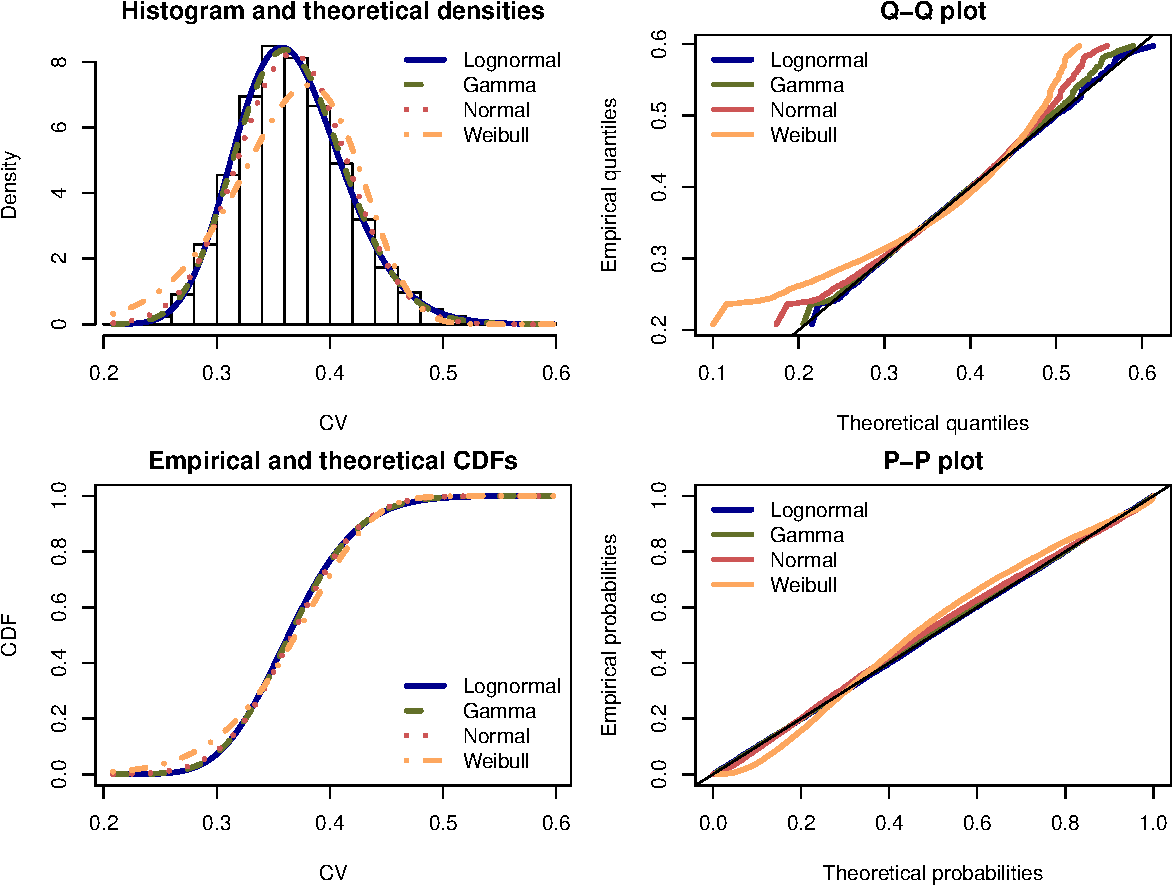
\includegraphics[width=1\linewidth]{Identifying-Heterogeneity-in-SAR-Data-with-New-Test-Statistics_files/figure-latex/Plot_MnADmedian_gamma-1} 
%DIFDELCMD < %%%
\DIFdelendFL \DIFaddbeginFL 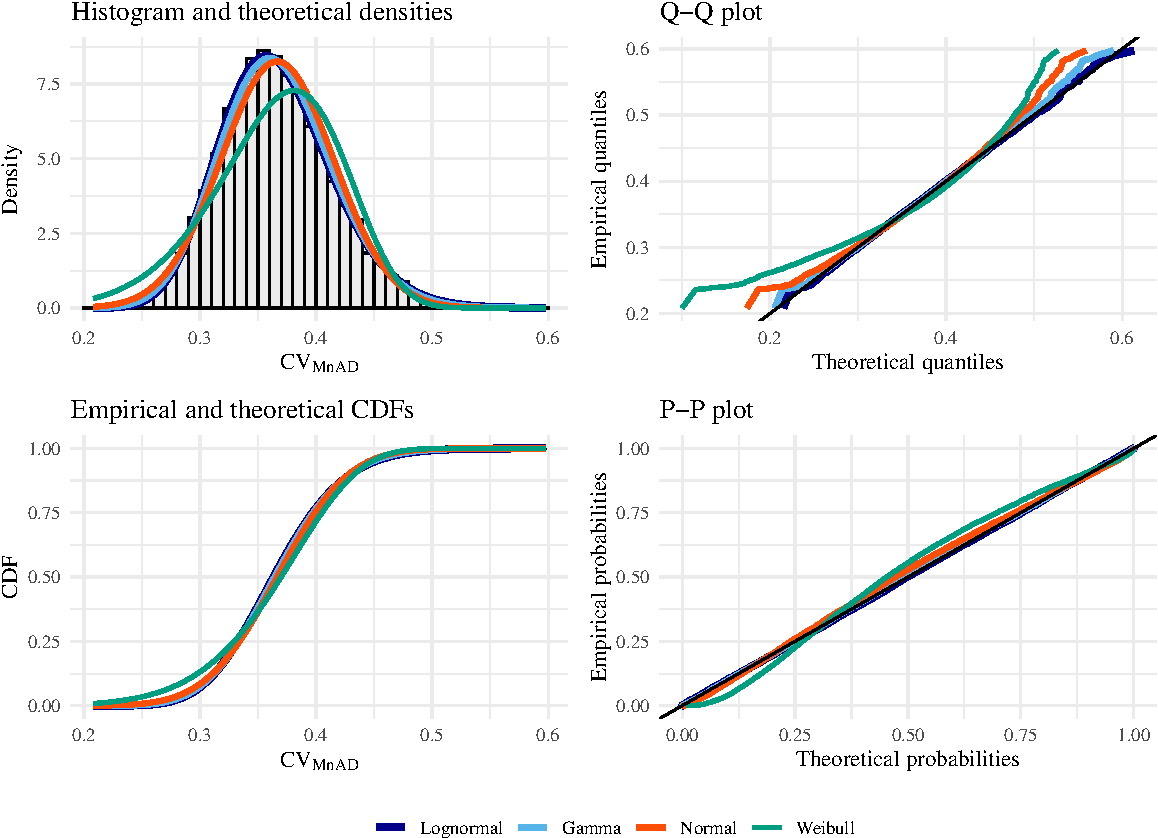
\includegraphics[width=1\linewidth]{R1-Identifying-Heterogeneity-in-SAR-Data-with-New-Test-Statistics_files/figure-latex/Plot_MnADmedian_gamma-1} 
\DIFaddendFL 

}

\caption{Goodness of fit plots for evaluating the best distribution with $\text{CV}_{\text{MnAD}}$ data from $\Gamma_{\text{SAR}}$ (under the null hypothesis), with  $n=49$, $L=5$, and $\mu=1$.}\label{fig:Plot_MnADmedian_gamma}
\end{figure}

\begin{figure}[hbt]
\DIFdelbeginFL %DIFDELCMD < 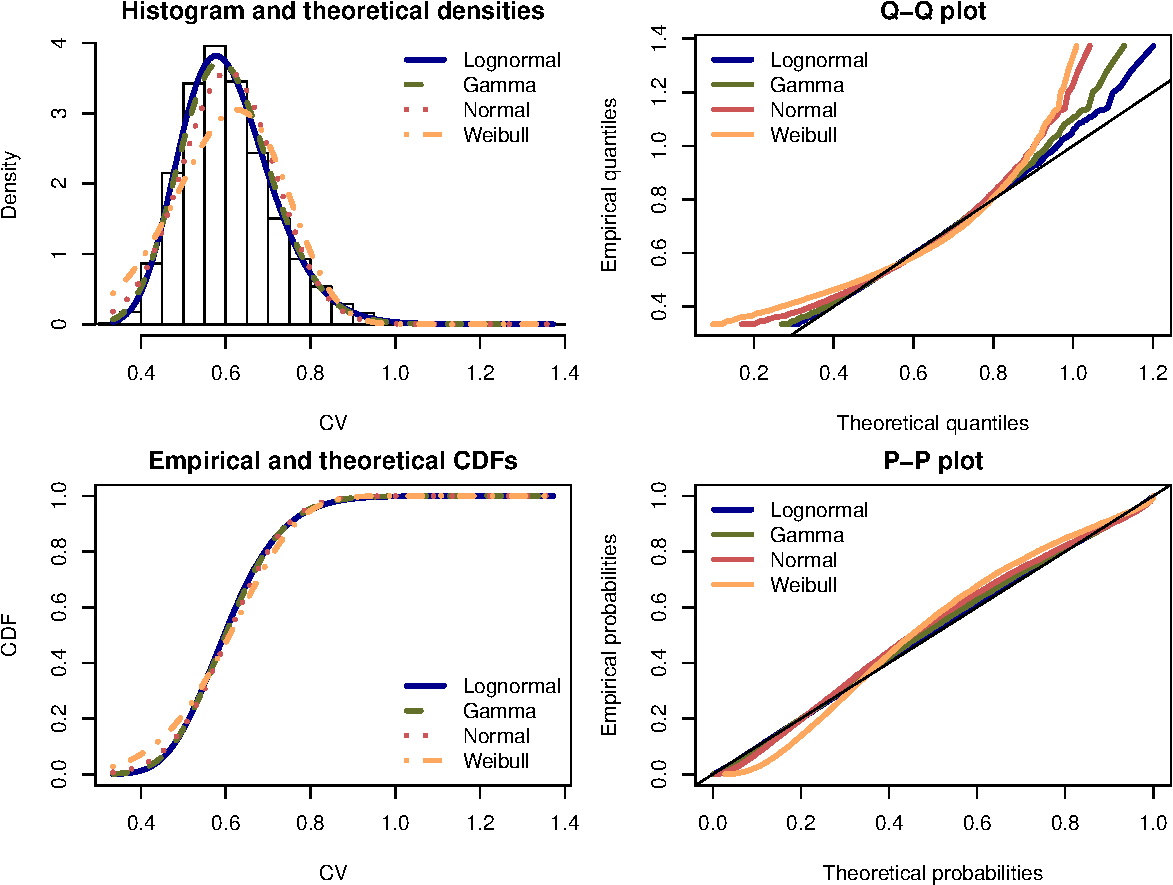
\includegraphics[width=1\linewidth]{Identifying-Heterogeneity-in-SAR-Data-with-New-Test-Statistics_files/figure-latex/Plot_madmed_gi0_MnADmedian-1} %%%
\DIFdelendFL \DIFaddbeginFL 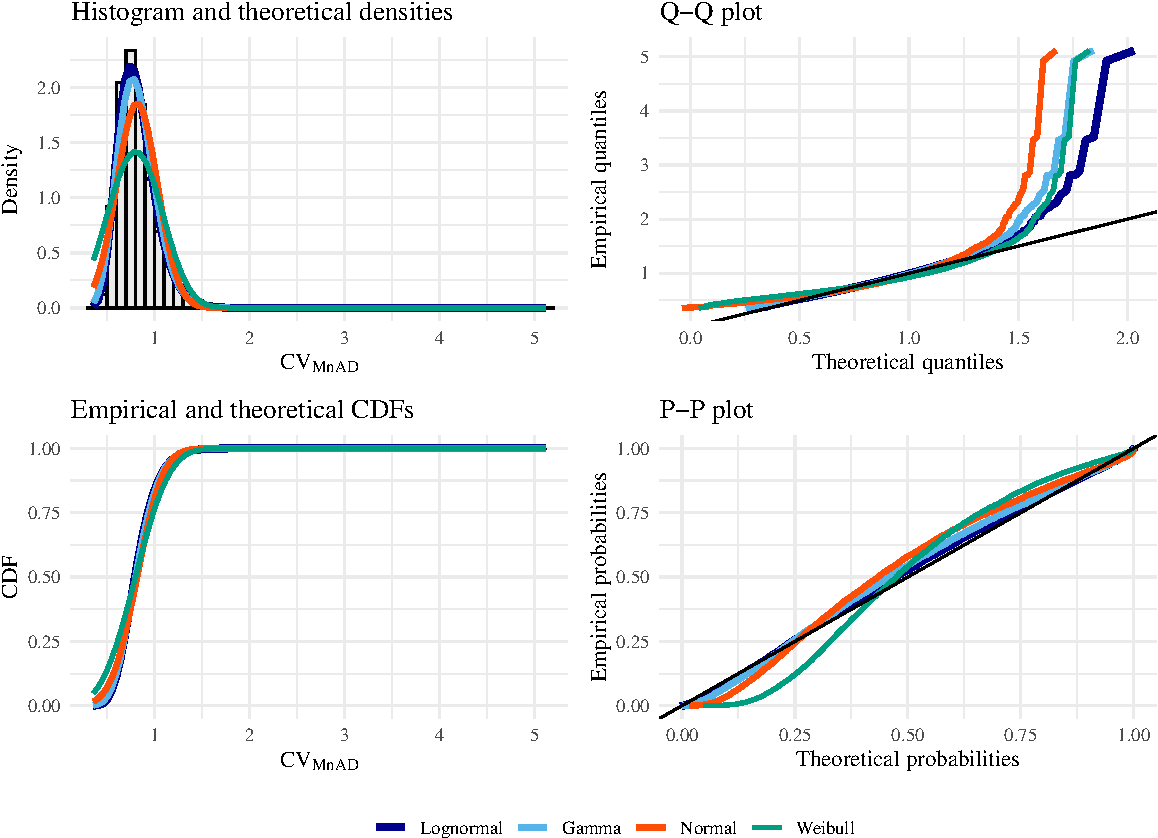
\includegraphics[width=1\linewidth]{R1-Identifying-Heterogeneity-in-SAR-Data-with-New-Test-Statistics_files/figure-latex/Plot_madmed_gi0_MnADmedian-1} \DIFaddendFL \caption{Goodness of fit plots for evaluating the best distribution with $CV_{\text{MnAD}}$ data from $G_I^0$ (under the alternative hypothesis), with  $n=49$, $L=5$, $\mu=1$, and $\alpha=-3$.}\label{fig:Plot_madmed_gi0_MnADmedian}
\end{figure}

\section{Results}\label{sec:Results}

This section presents the simulations we performed to evaluate the
proposed test statistics' performance, followed by applications to SAR
data.

\subsection{Simulated Data}\label{simulated-data}

Figure~\ref{fig:sim_Phantom}(a) shows the phantom with dimensions of
\(500\times500\) pixels. It was proposed by~\citet{Gomez2017} as a tool
to assess the performance of speckle-reduction filters.

Figure~\ref{fig:sim_Phantom}(b) shows the simulated image, where each
small phantom displaying texture variations. The observations are
independent draws from the \(G^0_I\) distribution~\eqref{E:gi02}, with
\(L = 5\) and varying \(\alpha\) and \(\mu\), annotated in the image for
each quadrant. Light regions correspond to textured observations
(heterogeneous), while darker regions represent textureless areas
(homogeneous).

The \(\alpha\) parameter of the \(G_I^0\) distribution is essential for
interpreting texture characteristics. Values near zero greater than
\(-3\) suggest extremely textured targets, such as urban
zones~\cite{Frery2019a}. As the value decreases, it indicates regions
with moderate texture (in the \(\left[-6,-3\right]\) region), related to
forest zones, while values below \(-6\) correspond to textureless
regions, such as pasture, agricultural fields, and water
bodies~\cite{Neto2023}.

\begin{figure}[H]
\subfloat[\label{fig:sim_Phantom-1}]{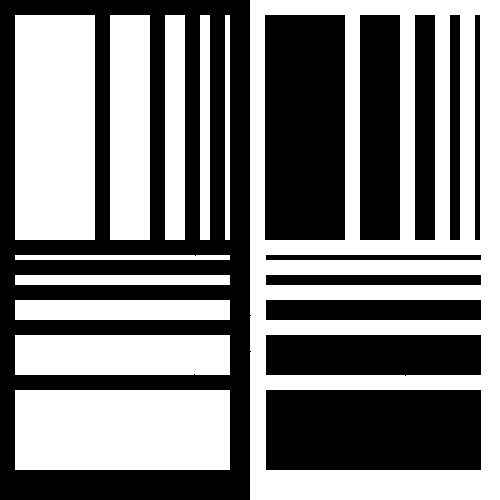
\includegraphics[width=60mm]{../Figures/PNG/Phantom1} }\subfloat[\label{fig:sim_Phantom-2}]{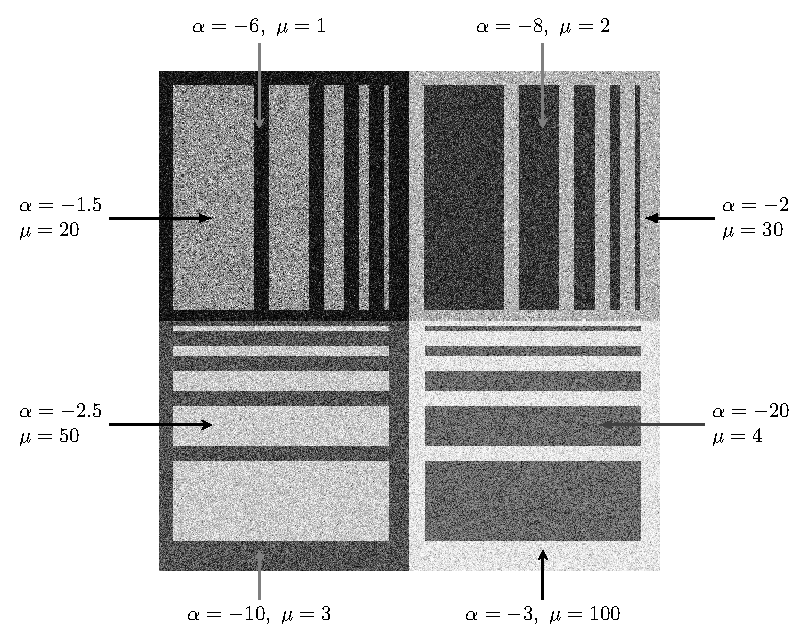
\includegraphics[width=80mm]{../Figures/PNG/Phantom_label/Phantom_labels} }\caption{Synthetic dataset: (\textbf{a}) Phantom. (\textbf{b}) Simulated image, varying $\alpha$ and $\mu$, with $L=5$. }\label{fig:sim_Phantom}
\end{figure}

We applied the three test statistics, namely
\(S_{\widetilde{H}_{\text{AO}}}(\bm{Z}; L)\), \(T_\text{CV}\), and
\(T_{\text{CV}_{\text{MnAD}}}\), to the simulated image using local
sliding windows of size \(7\times 7\), as shown in
Figures~\ref{fig:sim_results}(a)--(c).

\begin{figure}[H]
\subfloat[\label{fig:sim_results-1}]{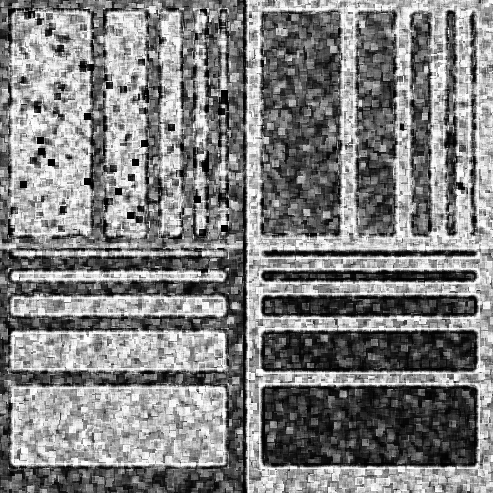
\includegraphics[width=45mm]{../Figures/PNG/Entropy_Phantom_4_z1_200} }\subfloat[\label{fig:sim_results-2}]{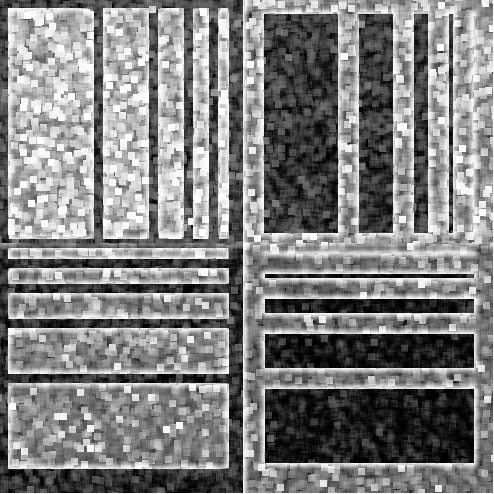
\includegraphics[width=45mm]{../Figures/PNG/cv_Phantom_4_z1} }\subfloat[\label{fig:sim_results-3}]{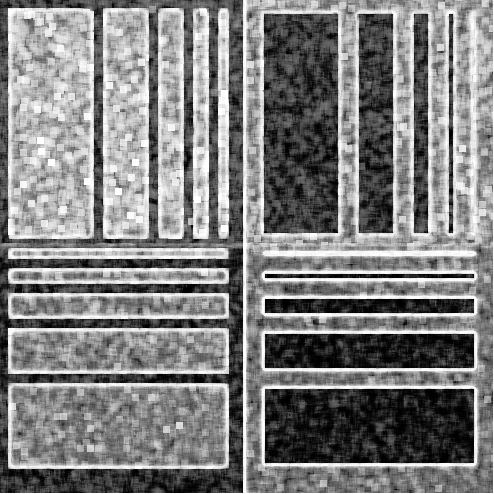
\includegraphics[width=45mm]{../Figures/PNG/mnad_Phantom_z1} }\caption{Results of applying the test statistics: (\textbf{a}) $S_{\widetilde{H}_{\text{AO}}}(\bm{Z}; L)$, (\textbf{b})  $T_\text{CV}$, and (\textbf{c})   $T_{\text{CV}_{\text{MnAD}}}$.}\label{fig:sim_results}
\end{figure}

The resulting \(p\)-values for each test are shown in
Figures~\ref{fig:sim_SAR_Images}(a)--(c). In
Figures~\ref{fig:sim_SAR_Images_p05}(a)--(c), maps are depicted using a
color table between black, gray levels, and white. All \(p\)-values
above \(0.05\) are represented in white (indicating no evidence to
reject the null hypothesis), while those below \(0.05\) are shown in
black (indicating evidence to reject the hypothesis). We notice that the
\(S_{\widetilde{H}_{\text{AO}}}(\bm{Z}; L)\) performs significantly
better than the other tests in identifying heterogeneous areas in the
simulated image.

\begin{figure}[H]
\subfloat[\label{fig:sim_SAR_Images-1}]{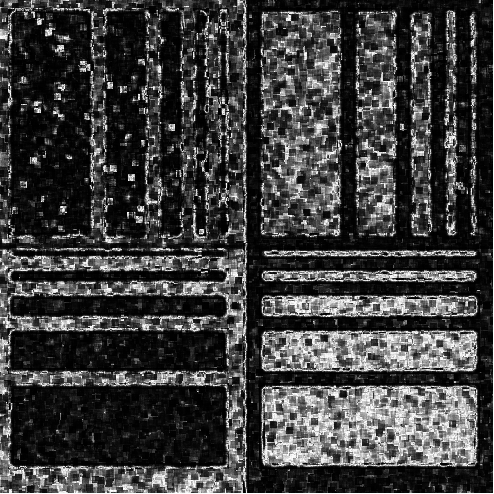
\includegraphics[width=45mm]{../Figures/PNG/H_pvalue_Phantom_4_z1_200b} }\subfloat[\label{fig:sim_SAR_Images-2}]{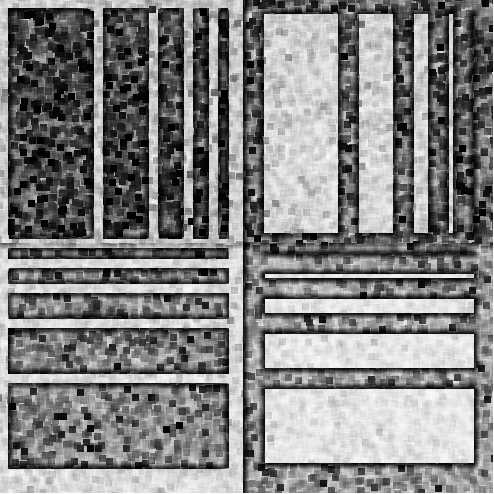
\includegraphics[width=45mm]{../Figures/PNG/cv_pvalues_Phantom_4_z1} }\subfloat[\label{fig:sim_SAR_Images-3}]{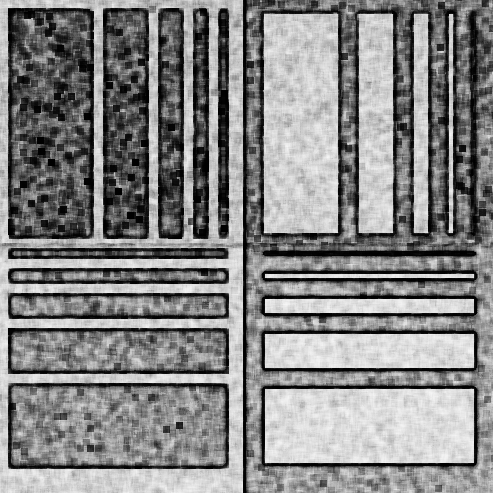
\includegraphics[width=45mm]{../Figures/PNG/mnad_p_values_Phantom_mnad_7_z1} }\caption{Map of $p$-values: (\textbf{a}) $S_{\widetilde{H}_{\text{AO}}}(\bm{Z}; L)$, (\textbf{b})  $T_\text{CV}$, and (\textbf{c}) $T_{\text{CV}_{\text{MnAD}}}$.}\label{fig:sim_SAR_Images}
\end{figure}
\begin{figure}[H]
\subfloat[ \label{fig:sim_SAR_Images_p05-1}]{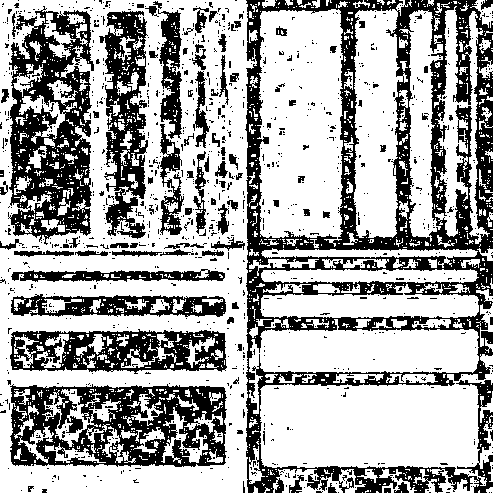
\includegraphics[width=45mm]{../Figures/PNG/H_005_Phantom_4_z1_AO_200b} }\subfloat[ \label{fig:sim_SAR_Images_p05-2}]{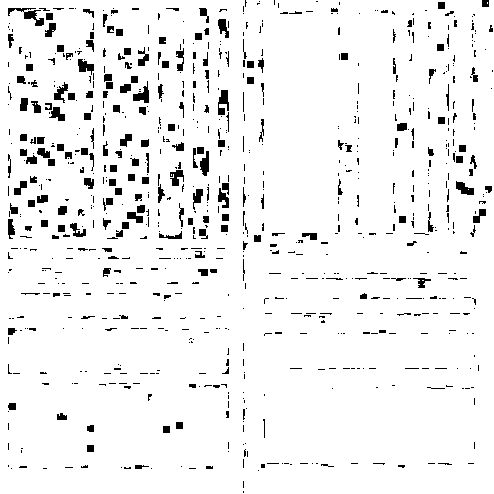
\includegraphics[width=45mm]{../Figures/PNG/cv_005_pvalues_Phantom_4_z1} }\subfloat[ \label{fig:sim_SAR_Images_p05-3}]{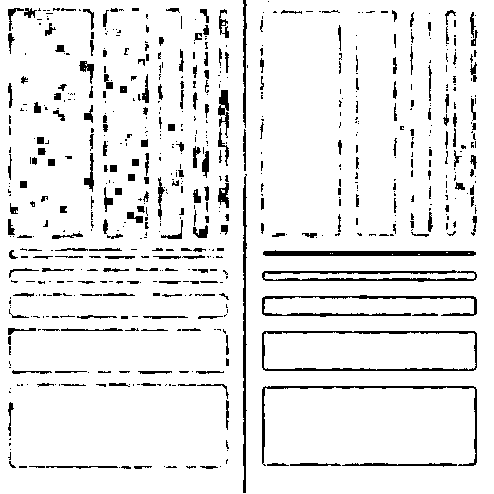
\includegraphics[width=45mm]{../Figures/PNG/mnad_005_Phantom_7_z1} }\caption{Results for a threshold of $0.05$ of the $p$-value: (\textbf{a}) $S_{\widetilde{H}_{\text{AO}}}(\bm{Z}; L)$, (\textbf{b})  $T_\text{CV}$, and (\textbf{c})   $T_{\text{CV}_{\text{MnAD}}}$.}\label{fig:sim_SAR_Images_p05}
\end{figure}

\subsection{SAR Data}\label{sar-data}

We evaluated the proposed test statistics using \DIFdelbegin \DIFdel{three }\DIFdelend \DIFaddbegin \DIFadd{four }\DIFaddend SAR images: one of
\DIFdelbegin \DIFdel{the coast of }\DIFdelend \DIFaddbegin \DIFadd{Rotterdam, Netherlands, acquired by the TerraSAR-X satellite with
Single-look Slant-range Complex (SSC) and high-resolution Spotlight-mode
(HS); another of the Coast of }\DIFaddend Jalisco, Mexico\DIFdelbegin \DIFdel{(with a spatial resolution of 20 m both
along azimuth and range directions) and }\DIFdelend \DIFaddbegin \DIFadd{; and }\DIFaddend two of Illinois, USA\DIFdelbegin \DIFdel{(with a
spatial resolution of \mbox{%DIFAUXCMD
\SI{10}{\meter} }\hskip0pt%DIFAUXCMD
both along azimuth and range
directions)}\DIFdelend ,
acquired by the Sentinel-1B \DIFdelbegin \DIFdel{satellite operating in C-band, with
VV polarization and intensity format.
The first two images have a
size of \(512 \times 512\) pixels, while the third has
\(1024 \times 1024\) pixels, and they }\DIFdelend \DIFaddbegin \DIFadd{in Ground Range Detected (GRD) format, with
Extra Wide-swath mode (EW) and Strip Map mode (SM).
Table~\ref{tab:table_param} provides detailed parameters of the selected
SAR images. They }\DIFaddend contain mountainous areas, agricultural regions, water
bodies, and urban areas, as shown in
Figures~\ref{fig:real_SAR_Images_coe}(a)--(\DIFdelbegin \DIFdel{c}\DIFdelend \DIFaddbegin \DIFadd{d}\DIFaddend ).

\DIFaddbegin \DIFadd{We used the number of looks \(L\) informed in the SNAP (Sentinel
Application Platform) metadata: the product of azimuth and range looks.
This value is close to the equivalent number of looks calculated as the
ratio of the squared sample mean to the sample variance in areas with
fully-developed speckle. }\renewcommand{\arraystretch}{2}\\

\begin{table}[H]
\centering\centering
\caption{\label{tab:table_param}\DIFaddFL{Parameters of selected SAR images.}}
\resizebox{\ifdim\width>\linewidth\linewidth\else\width\fi}{!}{
\fontsize{13}{15}\selectfont
\begin{tabu} to \linewidth {>{\centering\arraybackslash}p{3.5cm}>{\centering\arraybackslash}p{3cm}>{\centering\arraybackslash}p{2cm}>{\centering\arraybackslash}p{1cm}>{\centering\arraybackslash}p{2cm}>{\centering\arraybackslash}p{2.5cm}>{\centering\arraybackslash}p{1cm}>{\centering\arraybackslash}p{3cm}>{\centering\arraybackslash}p{3cm}}
\toprule
\multicolumn{1}{c}{\textbf{Site}} & \multicolumn{1}{c}{\textbf{Mission}} & \multicolumn{1}{c}{\textbf{Mode}} & \multicolumn{1}{c}{\textbf{Band}} & \multicolumn{1}{c}{\textbf{Polarization}} & \multicolumn{1}{c}{\textbf{Size}} & \multicolumn{1}{c}{$\bm{L}$} & \multicolumn{1}{c}{\textbf{Resolution Rg/Az [m]} } & \multicolumn{1}{c}{\textbf{Acquisition Date}}\\
\midrule
Rotterdam & TerraSAR-X & HS & X & HH & $512\times512$ & $1$ & $0.85/0.85$ & 06-12-2018\\
Coast of Jalisco & Sentinel-1B & GRD EW & C & VV & $512\times512$ & $18$ & $40/40$ & 29-08-2021\\
Illinois-Region 1 & Sentinel-1B & GRD SM & C & VV & $512\times512$ & $36$ & $10/10$ & 30-06-2020\\
Illinois-Region 2 & Sentinel-1B & GRD SM & C & VV & $1024\times1024$ & $36$ & $10/10$ & 28-08-2021\\
\bottomrule
\end{tabu}}
\end{table}

\DIFadd{Figures~\ref{fig:optical_Images}(a)--(d) show the optical images
obtained from Sentinel-2 L2A in true colors (composition of RGB
channels) for the corresponding SAR images, with acquisition dates as
follows: Rotterdam (20-12-2018), Coast of Jalisco (05-09-2021),
Illinois-Region 1 (25-06-2020), and Illinois-Region 2 (01-08-2021).
These optical images facilitate the interpretation of the results,
making it easier to distinguish between homogeneous and heterogeneous
regions.
}

\DIFaddend \begin{figure}[H]
\DIFdelbeginFL %DIFDELCMD < \subfloat[ \label{fig:real_SAR_Images_coe-1}]{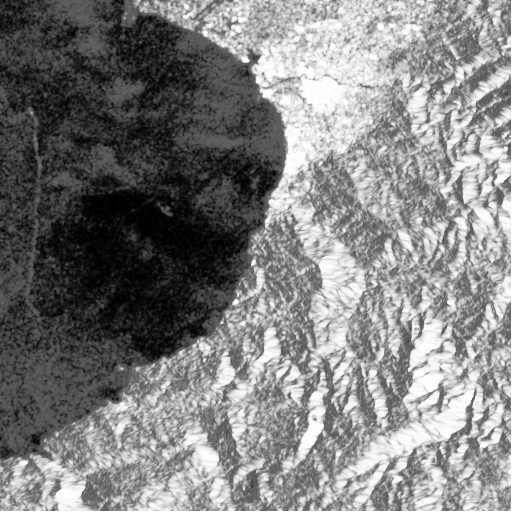
\includegraphics[width=45mm]{../Figures/PNG/Mexico_512} }\subfloat[ \label{fig:real_SAR_Images_coe-2}]{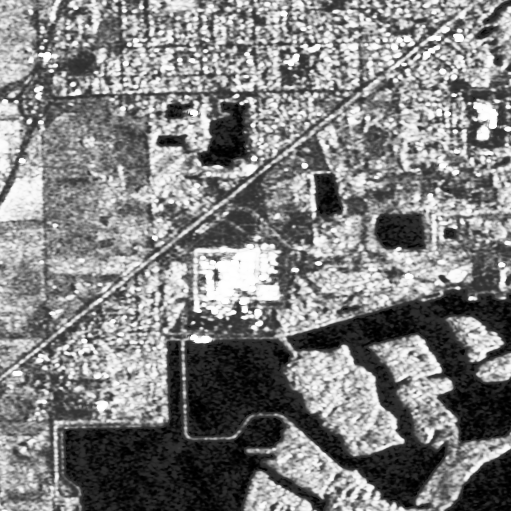
\includegraphics[width=45mm]{../Figures/PNG/lake_512} }\subfloat[ \label{fig:real_SAR_Images_coe-3}]{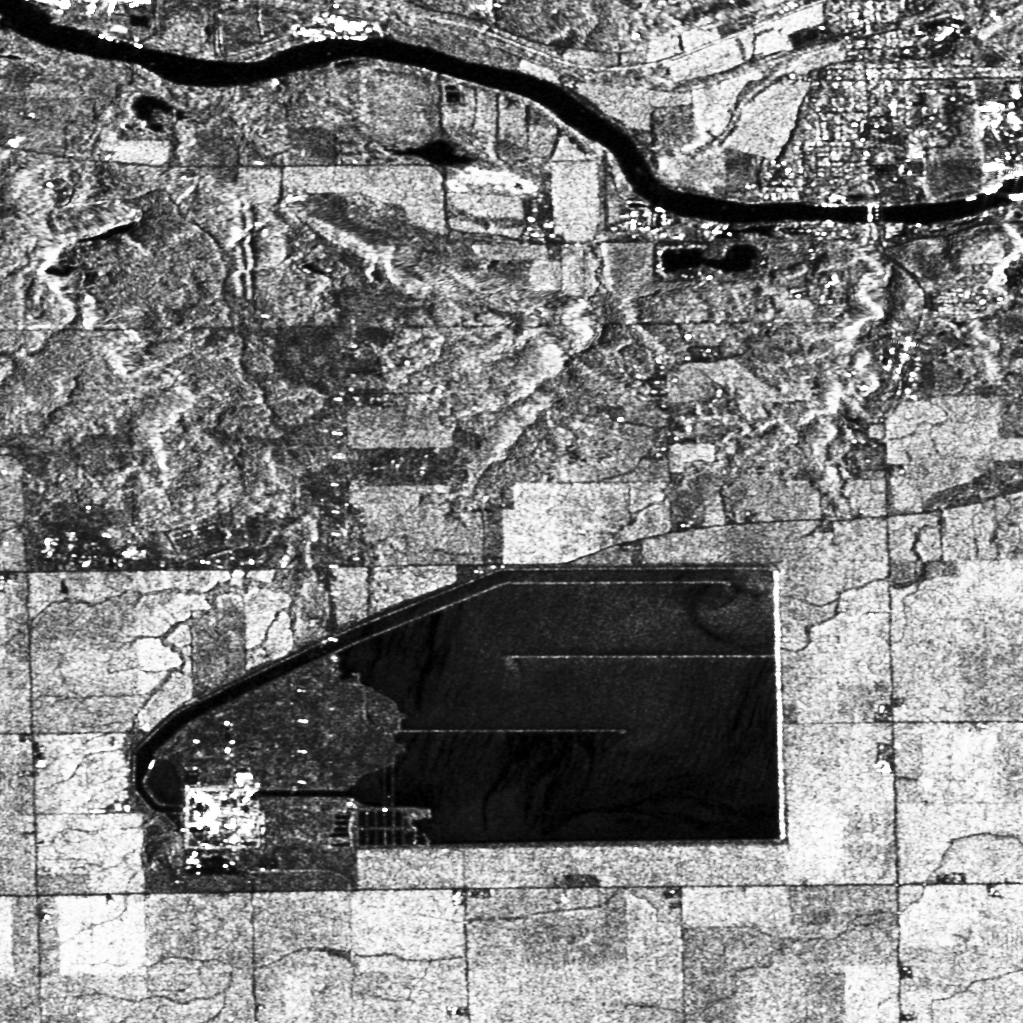
\includegraphics[width=45mm]{../Figures/PNG/Illinois_1024_36L} }%%%
\DIFdelendFL \DIFaddbeginFL 

{\centering \subfloat[ \label{fig:real_SAR_Images_coe-1}]{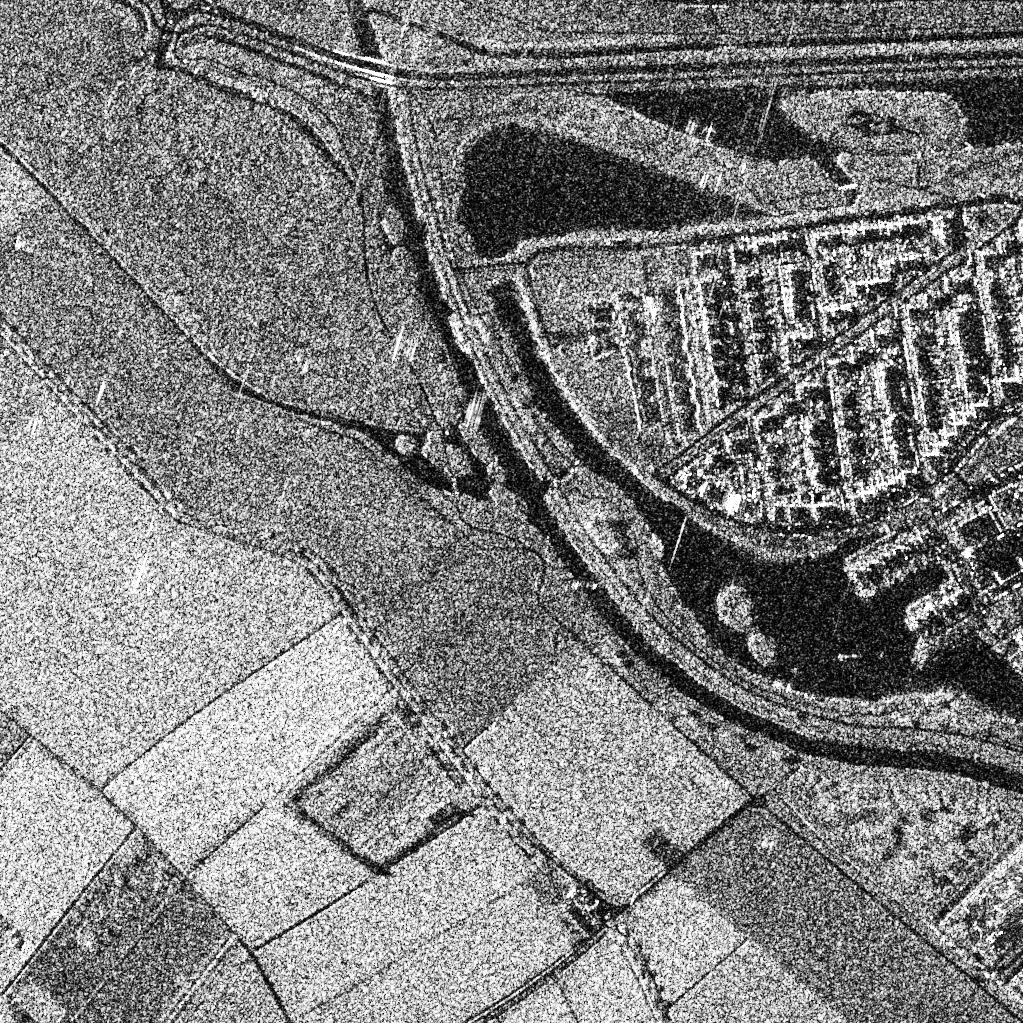
\includegraphics[width=45mm]{../Figures/PNG/Rotterdam_1024} }\subfloat[ \label{fig:real_SAR_Images_coe-2}]{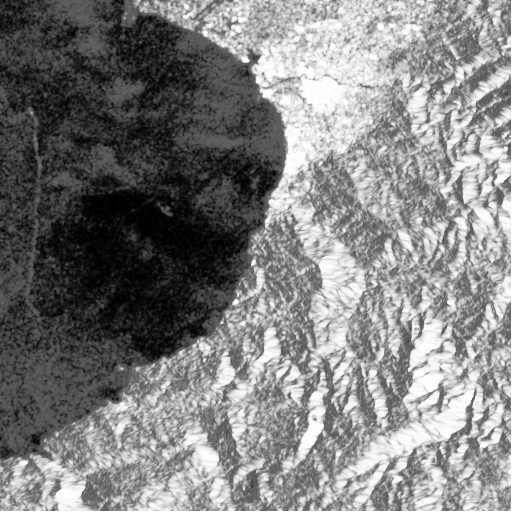
\includegraphics[width=45mm]{../Figures/PNG/Mexico_512} }\newline\subfloat[ \label{fig:real_SAR_Images_coe-3}]{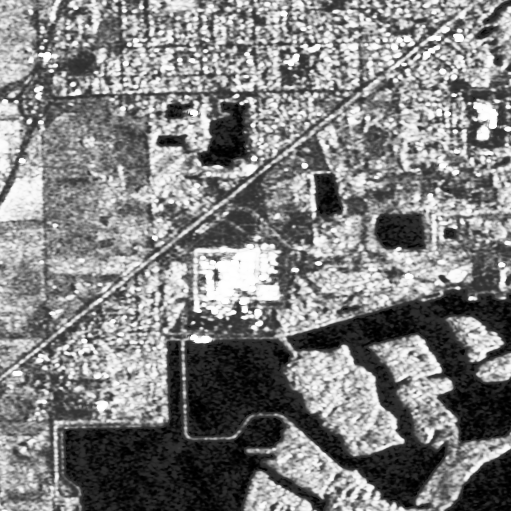
\includegraphics[width=45mm]{../Figures/PNG/lake_512} }\subfloat[\label{fig:real_SAR_Images_coe-4}]{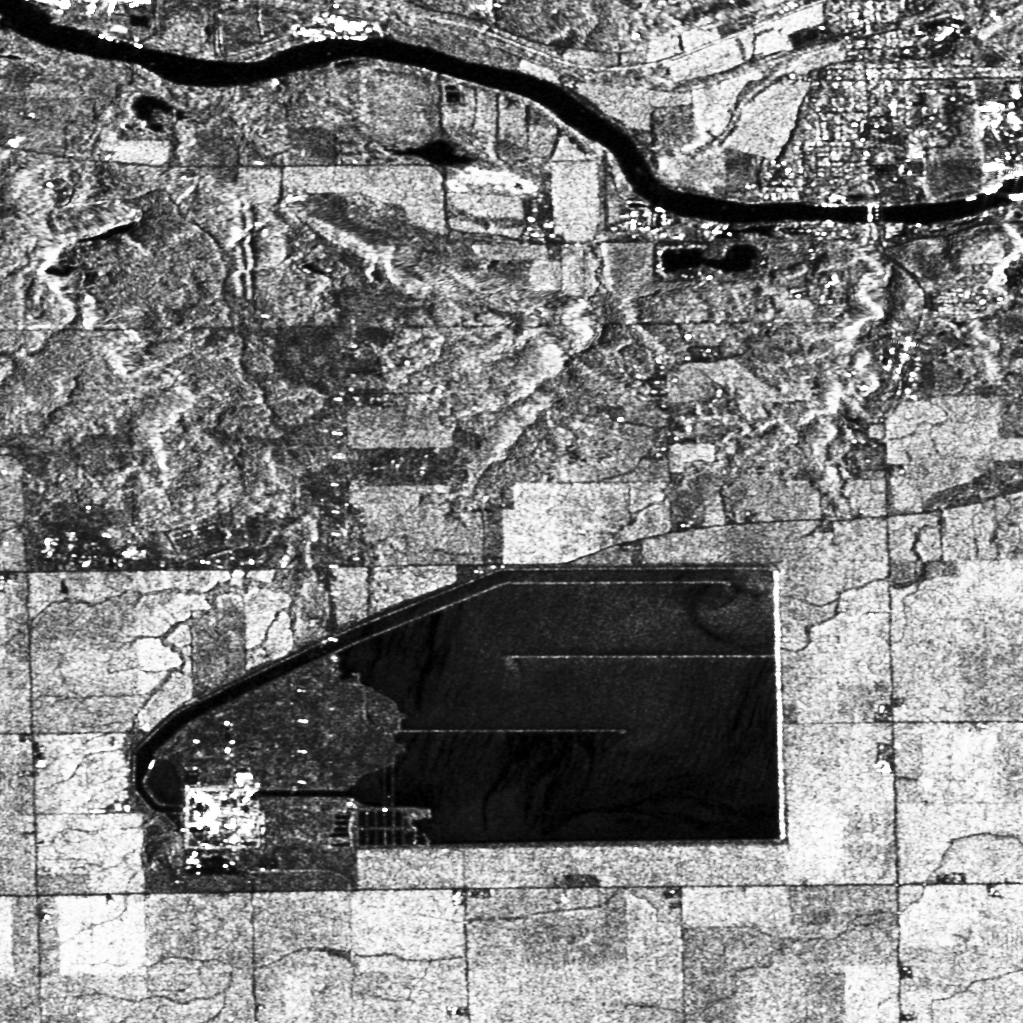
\includegraphics[width=45mm]{../Figures/PNG/Illinois_1024_36L} }\newline

}

\DIFaddendFL \caption{SAR images: (\textbf{a}) \DIFaddbeginFL \DIFaddFL{Rotterdam, (}\textbf{\DIFaddFL{b}}\DIFaddFL{) }\DIFaddendFL Coast of Jalisco, \DIFdelbeginFL \DIFdelFL{with $L=18$. }\DIFdelendFL (\DIFdelbeginFL \textbf{\DIFdelFL{b}}%DIFAUXCMD
\DIFdelendFL \DIFaddbeginFL \textbf{\DIFaddFL{c}}\DIFaddendFL ) Illinois-Region 1, \DIFdelbeginFL \DIFdelFL{with $L=36$. \quad \quad \quad \quad \quad }\DIFdelendFL (\DIFdelbeginFL \textbf{\DIFdelFL{c}}%DIFAUXCMD
\DIFdelendFL \DIFaddbeginFL \textbf{\DIFaddFL{d}}\DIFaddendFL ) Illinois-Region \DIFdelbeginFL \DIFdelFL{2, with $L=36$. }\DIFdelendFL \DIFaddbeginFL \DIFaddFL{2.}\DIFaddendFL }\label{fig:real_SAR_Images_coe}
\end{figure}

\DIFaddbegin \begin{figure}[H]

{\centering \subfloat[ \label{fig:optical_Images-1}]{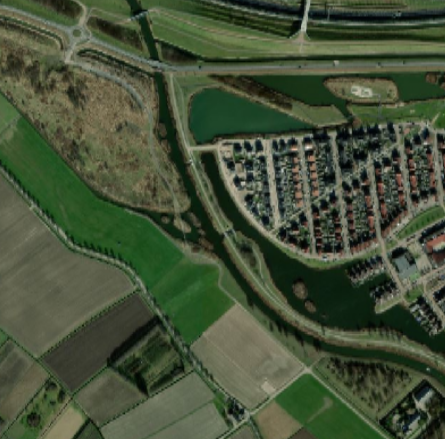
\includegraphics[width=45mm]{../Figures/PNG/Rotterdam} }\subfloat[ \label{fig:optical_Images-2}]{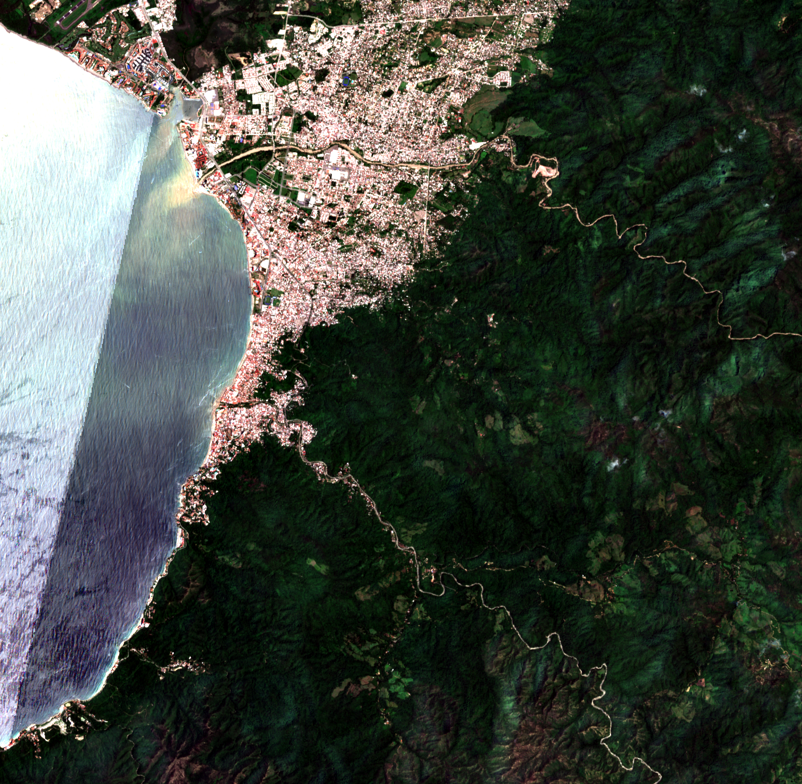
\includegraphics[width=45mm]{../Figures/PNG/Jalisco_o2} }\newline\subfloat[ \label{fig:optical_Images-3}]{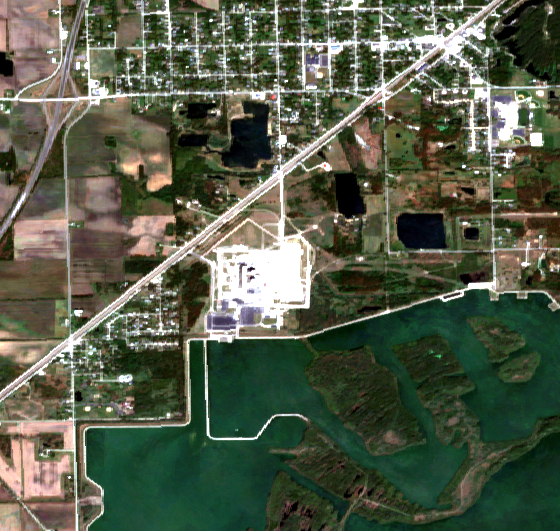
\includegraphics[width=47mm]{../Figures/PNG/Sentinel2_Illinois_lake} }\subfloat[ \label{fig:optical_Images-4}]{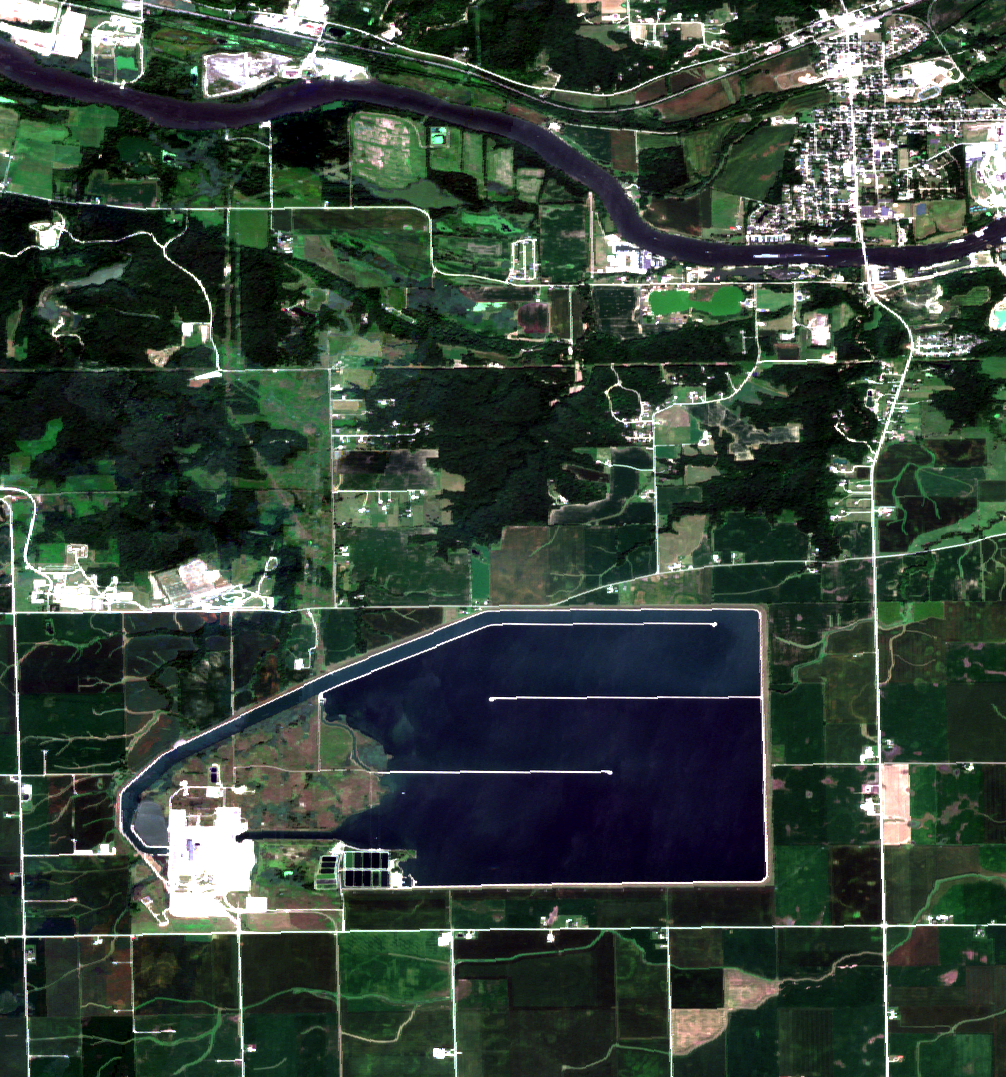
\includegraphics[width=42mm]{../Figures/PNG/Sentinel_2021_R2} }\newline

}

\caption{\DIFaddFL{Optical images: (}\textbf{\DIFaddFL{a}}\DIFaddFL{) Rotterdam, (}\textbf{\DIFaddFL{b}}\DIFaddFL{) Coast Jalisco, (}\textbf{\DIFaddFL{c}}\DIFaddFL{) Illinois-Region 1, (}\textbf{\DIFaddFL{d}}\DIFaddFL{) Illinois-Region 2.}}\label{fig:optical_Images}
\end{figure}

\DIFaddend The three statistical tests are applied to the SAR images using
\(7\times 7\) local sliding windows\DIFaddbegin \DIFadd{. This window size balances detailed
local information and sufficient number of data points}\DIFaddend , as illustrated
in Figures~\DIFaddbegin \DIFadd{\ref{fig:test_Rotterdam}, }\DIFaddend \ref{fig:real_images_test_Mexico},
\ref{fig:test_lake} and~\ref{fig:real_images_test_Illinois}.

The \(p\)-values obtained for each test are presented in
Figures~\DIFaddbegin \DIFadd{\ref{fig:Rotterdam_pvalue}, }\DIFaddend \ref{fig:Mexico_pvalue},
\ref{fig:lake_pvalue} and~\ref{fig:Illinois_crops_pvalue}, respectively.

In Figures~\DIFaddbegin \DIFadd{\ref{fig:Rotterdam_0.05}, }\DIFaddend \ref{fig:Mexico_crops_0.05},
\ref{fig:lake_0.05} and~\ref{fig:Illinois_crops_0.05}, the maps of
\(p\)-values composed of a linear gradient of black and white colors,
represent the decisions at a \SI{5}{\percent} significance level. Dark
areas represent values below \(0.05\), indicating evidence to reject the
null hypothesis and suggesting heterogeneity in these regions. In
contrast, values above 0.05 are represented as white areas, indicating
no evidence to reject the fully-developed speckle hypothesis.

\begin{figure}[H]
\DIFaddbeginFL \subfloat[\label{fig:test_Rotterdam-1}]{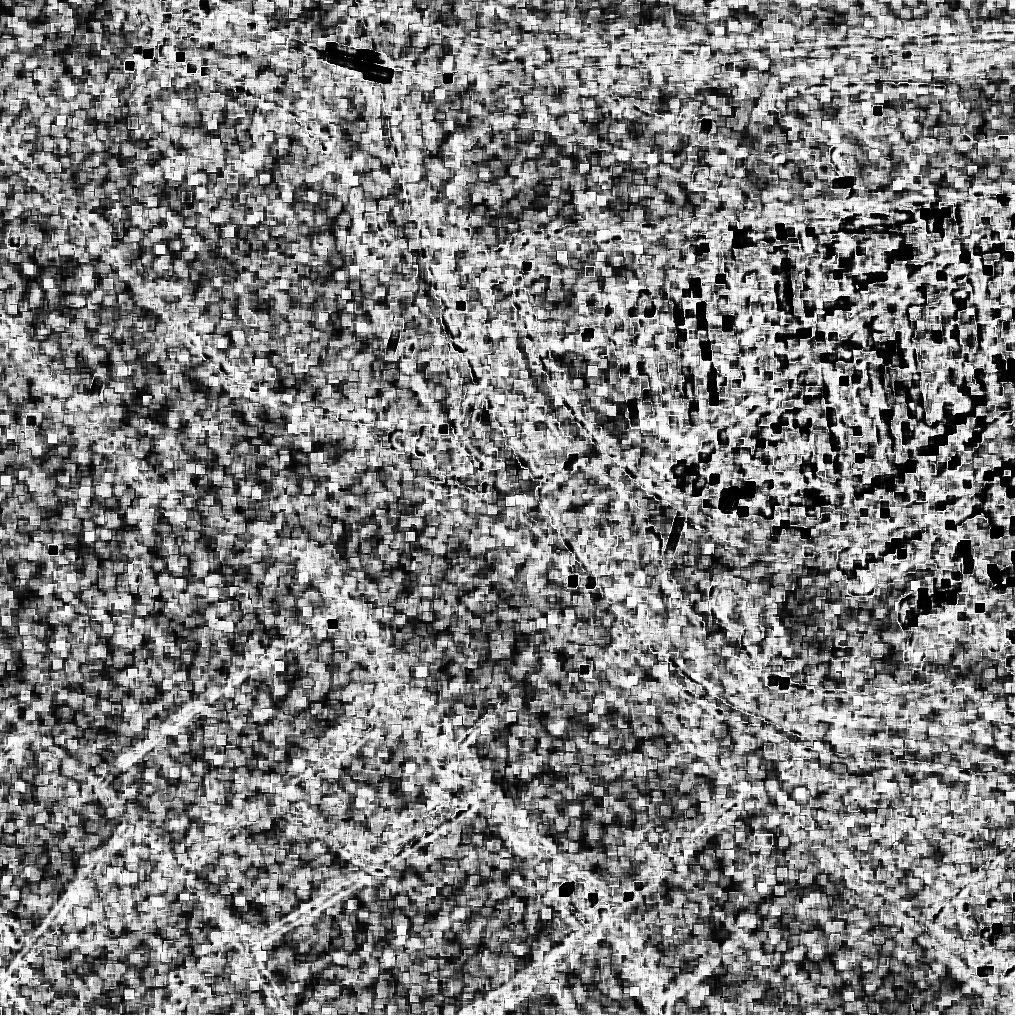
\includegraphics[width=45mm]{../Figures/PNG/Entropy_AO_Rotterdam_1024} }\subfloat[\label{fig:test_Rotterdam-2}]{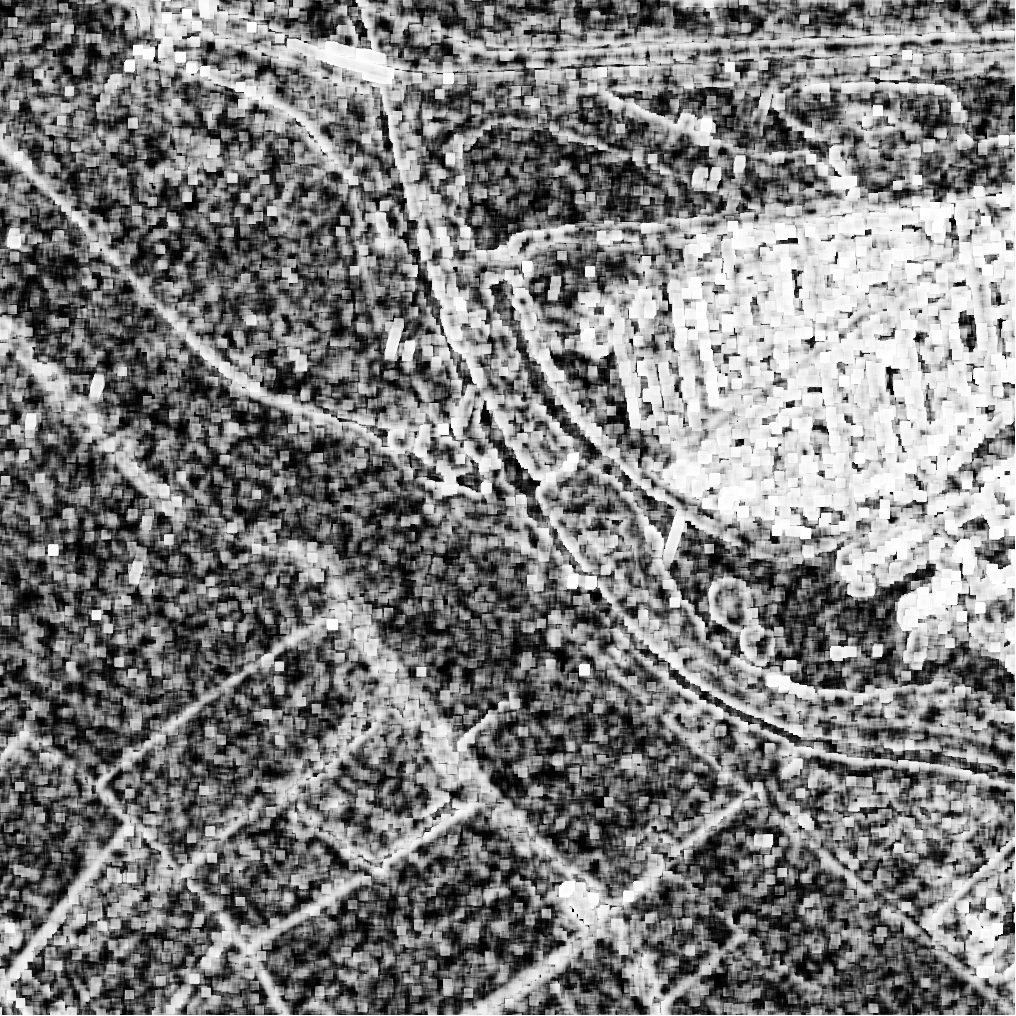
\includegraphics[width=45mm]{../Figures/PNG/cv_Rotterdam} }\subfloat[\label{fig:test_Rotterdam-3}]{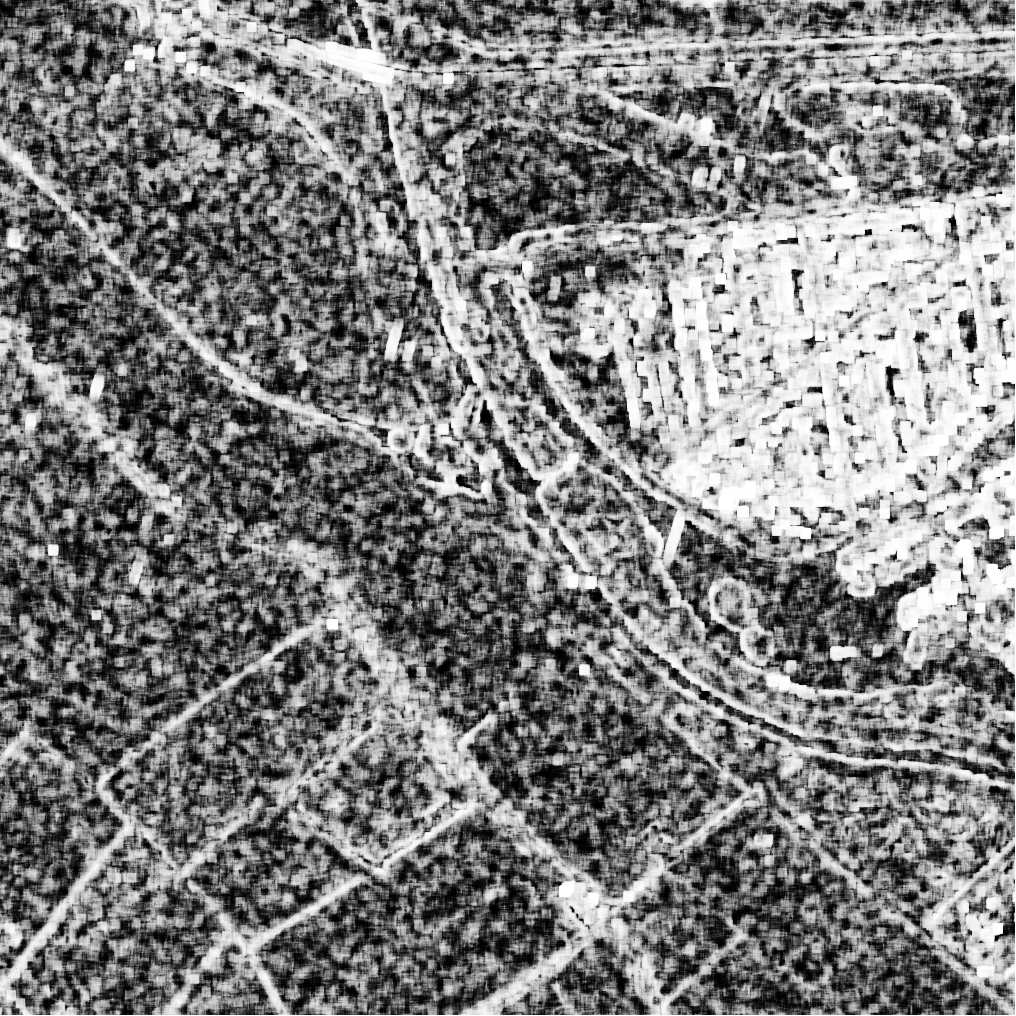
\includegraphics[width=45mm]{../Figures/PNG/mnad_Rotterdam} }\caption{\DIFaddFL{Results of applying the test statistics, Rotterdam: (}\textbf{\DIFaddFL{a}}\DIFaddFL{) $S_{\widetilde{H}_{\text{AO}}}(\bm{Z}; L)$, (}\textbf{\DIFaddFL{b}}\DIFaddFL{)  $T_\text{CV}$, and (}\textbf{\DIFaddFL{c}}\DIFaddFL{)   $T_{\text{CV}_{\text{MnAD}}}$.}}\label{fig:test_Rotterdam}
\end{figure}

\begin{figure}[H]
\subfloat[ \label{fig:Rotterdam_pvalue-1}]{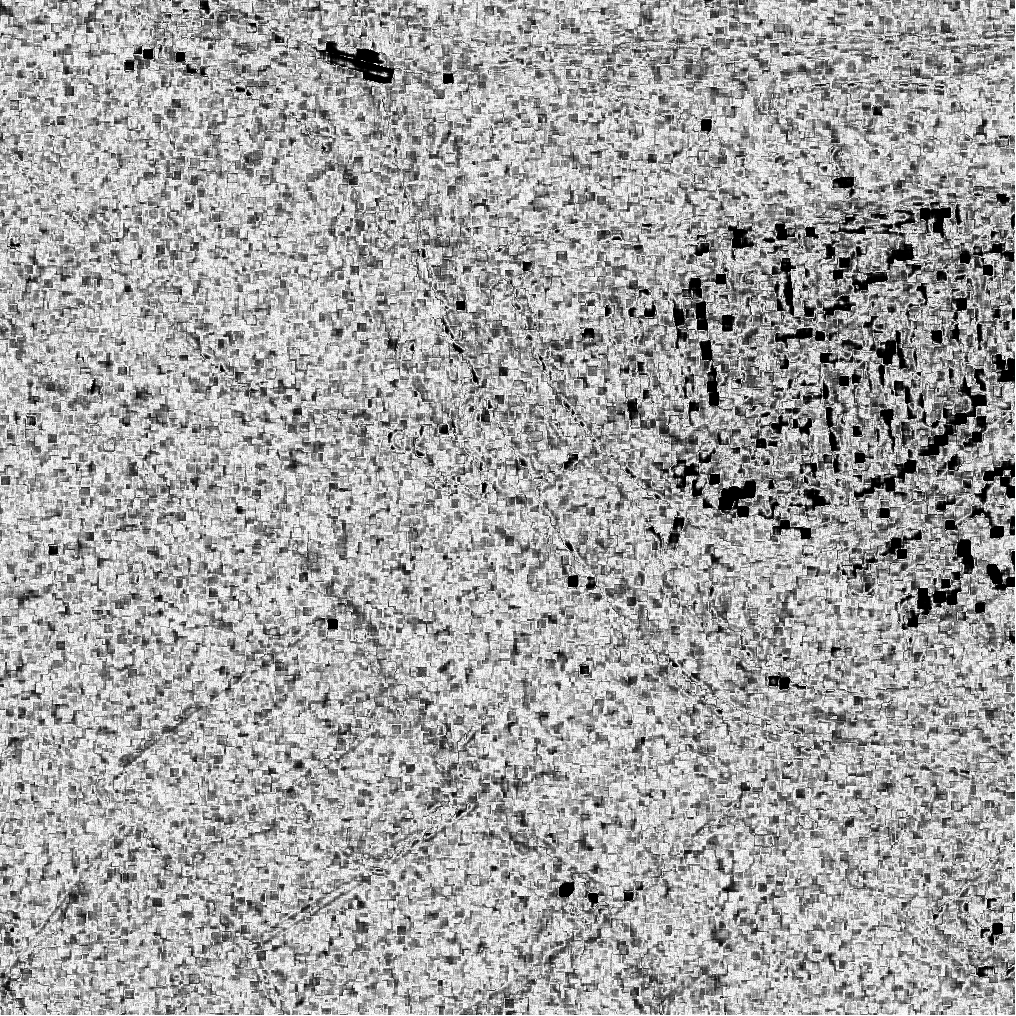
\includegraphics[width=45mm]{../Figures/PNG/H_pvalue_AO_Rotterdam_1024} }\subfloat[ \label{fig:Rotterdam_pvalue-2}]{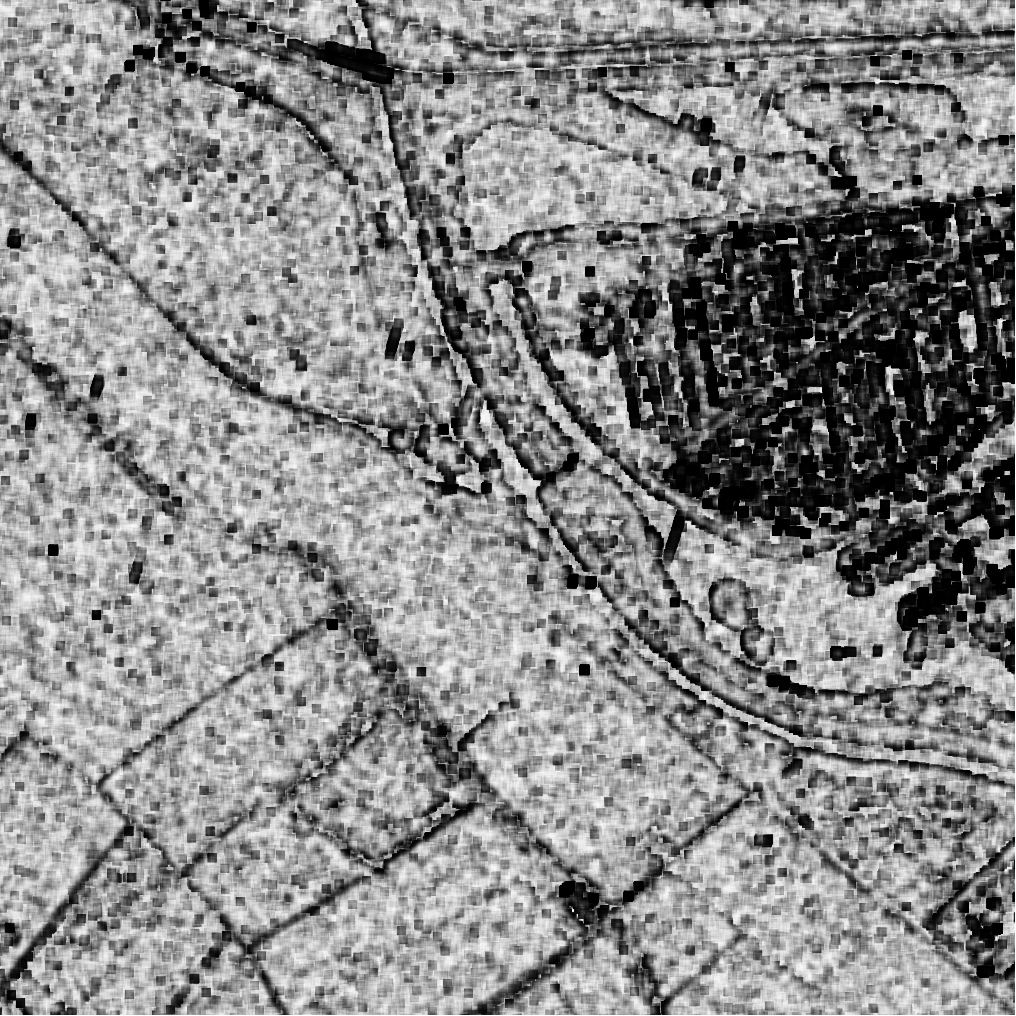
\includegraphics[width=45mm]{../Figures/PNG/cv_pvalues_Rotterdam} }\subfloat[ \label{fig:Rotterdam_pvalue-3}]{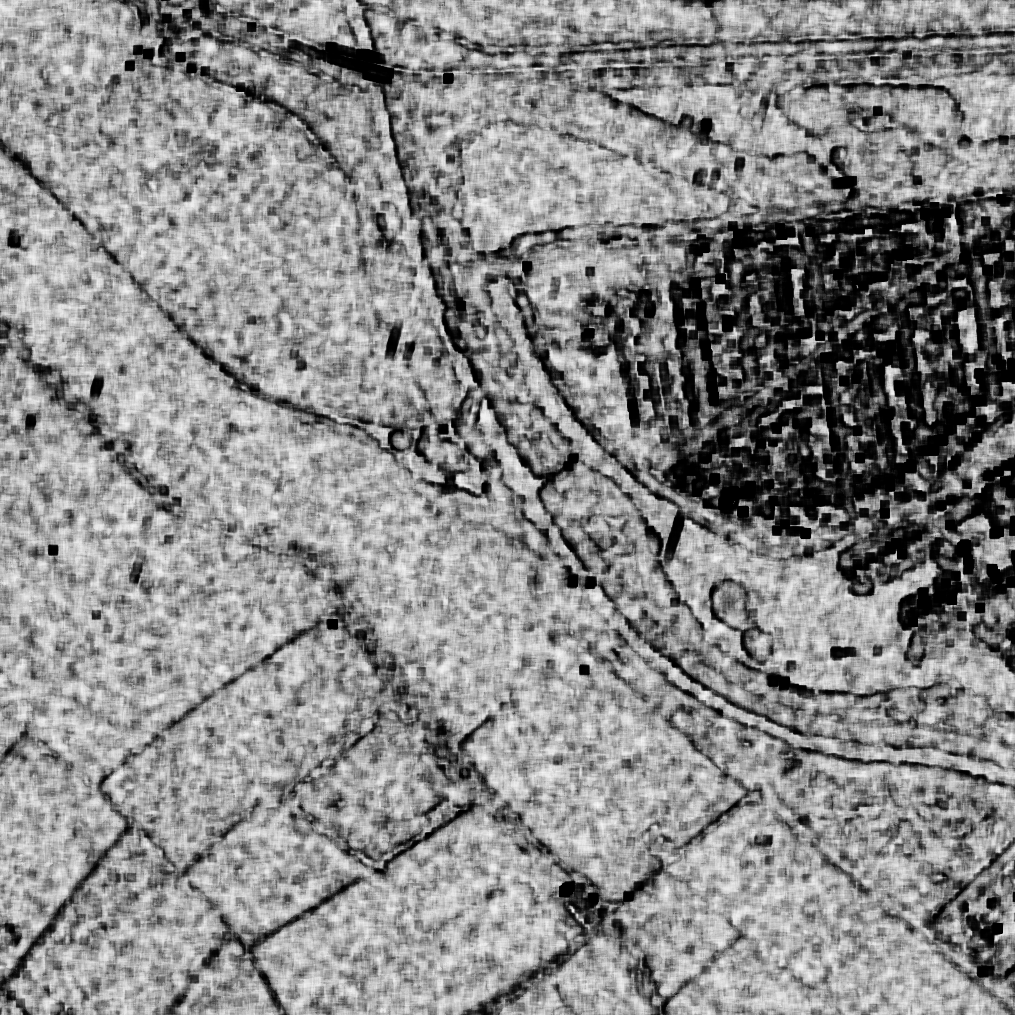
\includegraphics[width=45mm]{../Figures/PNG/mnad_p_values_Rotterdam} }\caption{\DIFaddFL{Map of $p$-values, Rotterdam: (}\textbf{\DIFaddFL{a}}\DIFaddFL{) $S_{\widetilde{H}_{\text{AO}}}(\bm{Z}; L)$. (}\textbf{\DIFaddFL{b}}\DIFaddFL{)  $T_\text{CV}$. (}\textbf{\DIFaddFL{c}}\DIFaddFL{)   $T_{\text{CV}_{\text{MnAD}}}$.}}\label{fig:Rotterdam_pvalue}
\end{figure}

\begin{figure}[H]
\subfloat[ \label{fig:Rotterdam_0.05-1}]{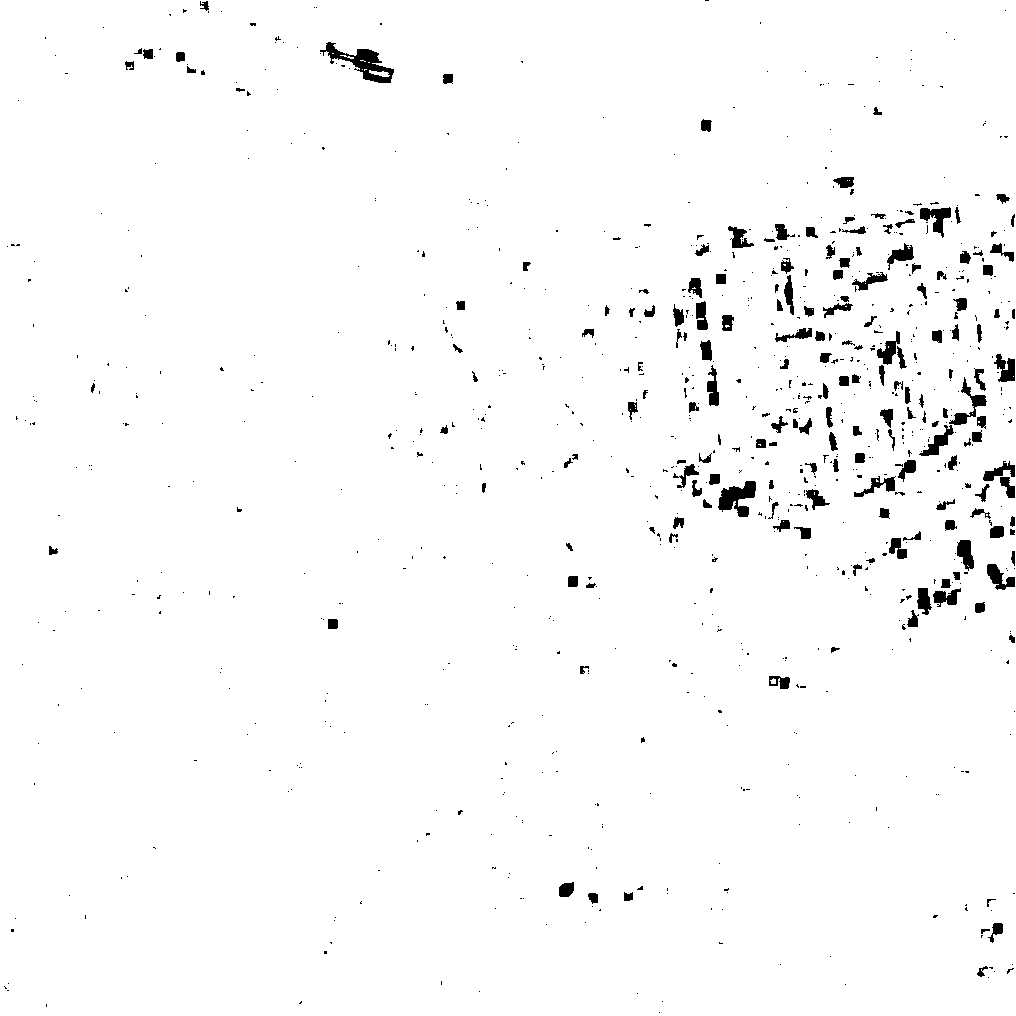
\includegraphics[width=45mm]{../Figures/PNG/H_005_AO_Rotterdam_1024} }\subfloat[ \label{fig:Rotterdam_0.05-2}]{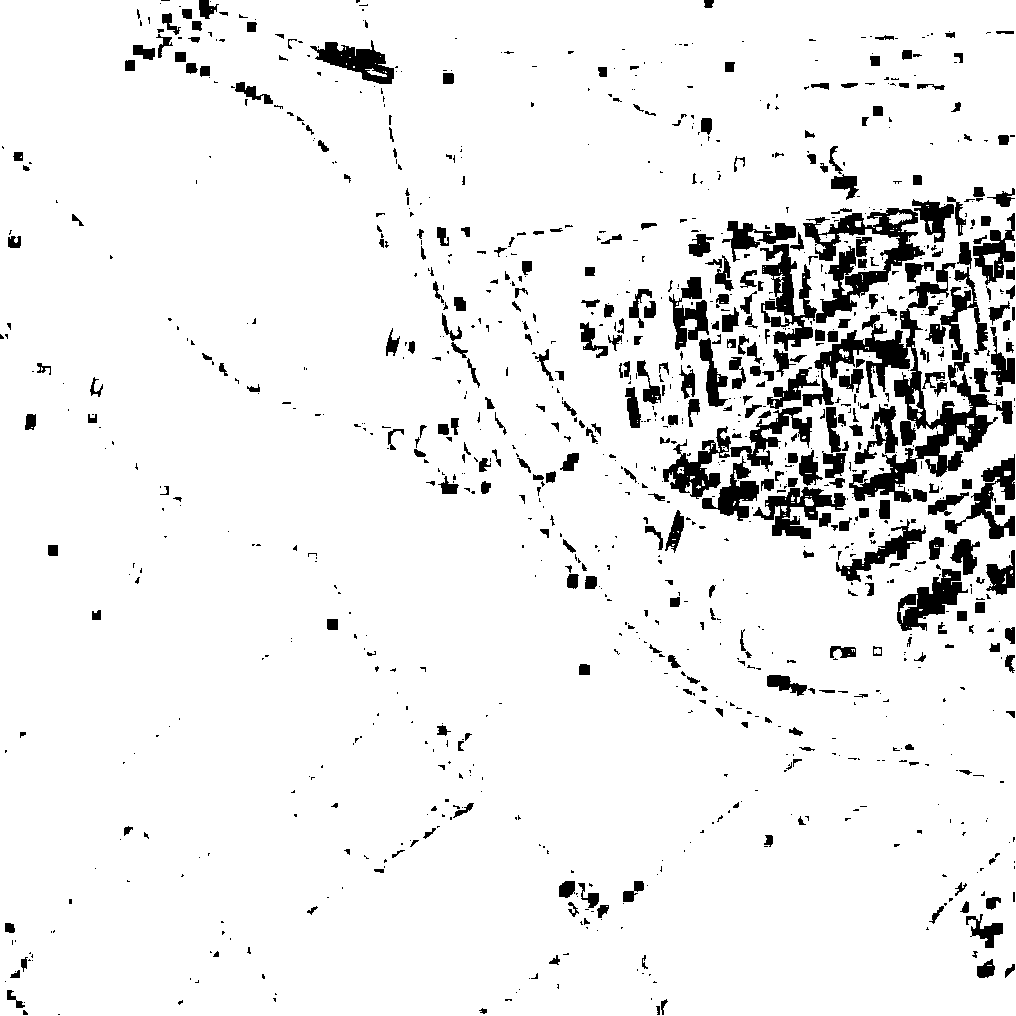
\includegraphics[width=45mm]{../Figures/PNG/cv_005_pvalues_Rotterdam} }\subfloat[ \label{fig:Rotterdam_0.05-3}]{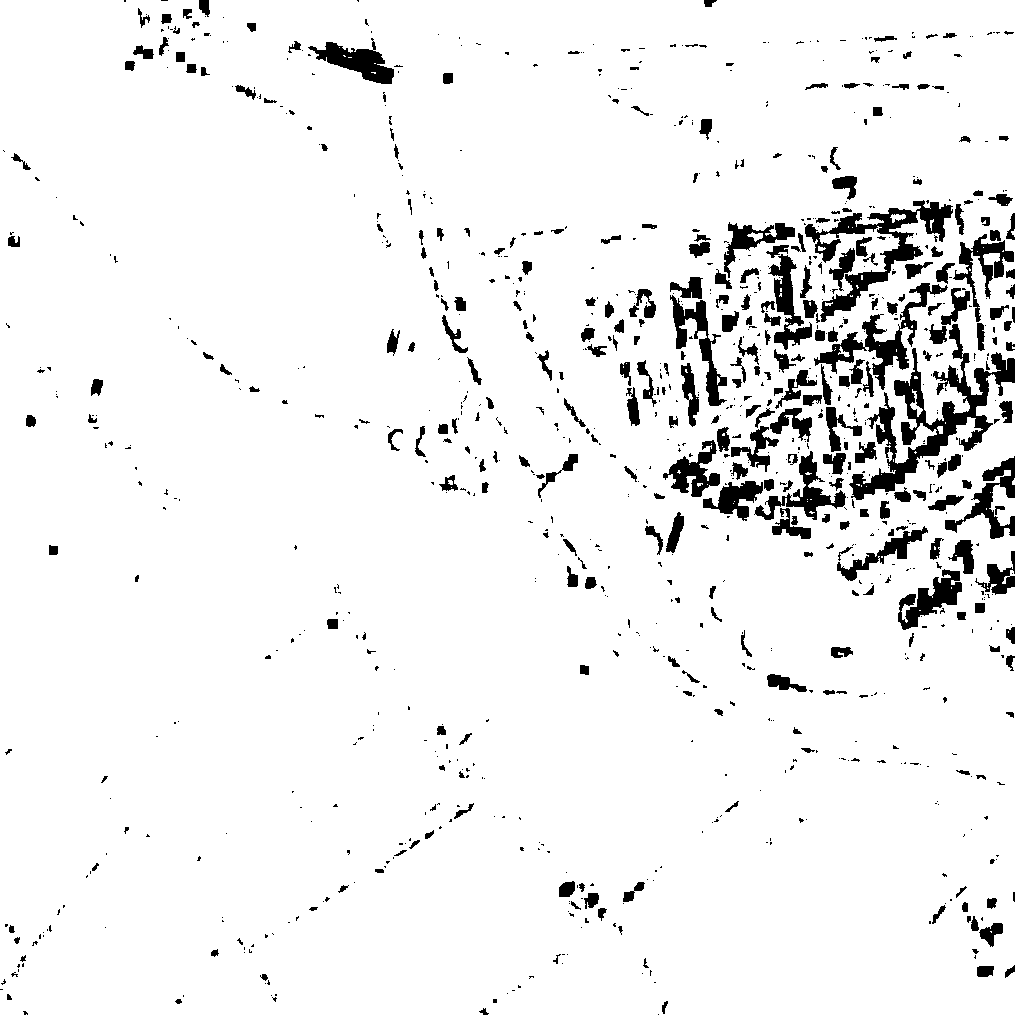
\includegraphics[width=45mm]{../Figures/PNG/mnad_005_Rotterdam} }\caption{\DIFaddFL{Results for a threshold of $0.05$ of the $p$-value, Rotterdam. (}\textbf{\DIFaddFL{a}}\DIFaddFL{) $S_{\widetilde{H}_{\text{AO}}}(\bm{Z}; L)$, (}\textbf{\DIFaddFL{b}}\DIFaddFL{) $T_\text{CV}$, and \quad \quad \quad \quad \quad (}\textbf{\DIFaddFL{c}}\DIFaddFL{)   $T_{\text{CV}_{\text{MnAD}}}$.}}\label{fig:Rotterdam_0.05}
\end{figure}

\begin{figure}[H]
\DIFaddendFL \subfloat[\label{fig:real_images_test_Mexico-1}]{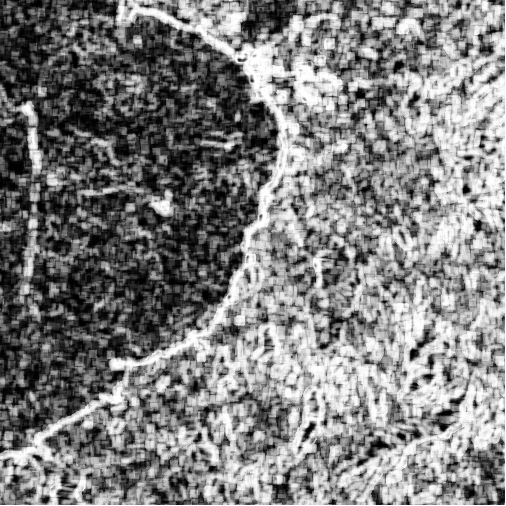
\includegraphics[width=45mm]{../Figures/PNG/Entropy_Mexico_512_18L_AO_200b} }\subfloat[\label{fig:real_images_test_Mexico-2}]{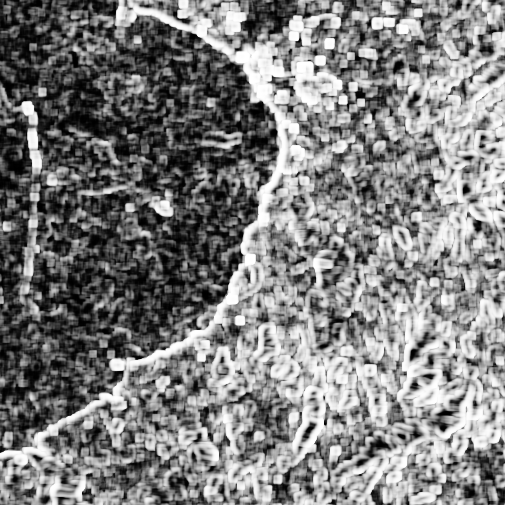
\includegraphics[width=45mm]{../Figures/PNG/cv_mexico_512} }\subfloat[\label{fig:real_images_test_Mexico-3}]{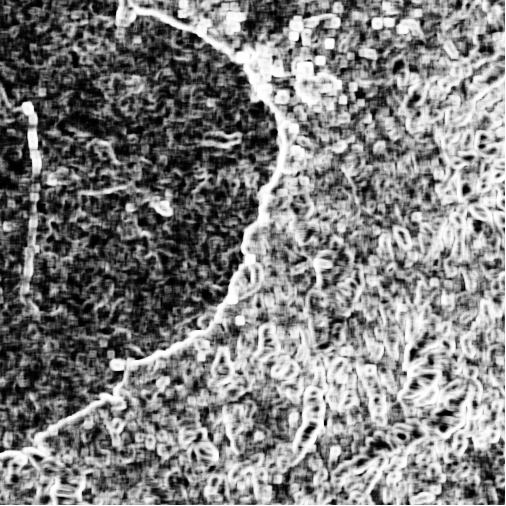
\includegraphics[width=45mm]{../Figures/PNG/mnad_mexico_512} }\caption{Results of applying the test statistics, Coast of Jalisco: (\textbf{a}) $S_{\widetilde{H}_{\text{AO}}}(\bm{Z}; L)$, (\textbf{b})  $T_\text{CV}$, and \quad \quad \quad \quad \quad (\textbf{c})   $T_{\text{CV}_{\text{MnAD}}}$.}\label{fig:real_images_test_Mexico}
\end{figure}

\begin{figure}[H]
\subfloat[ \label{fig:Mexico_pvalue-1}]{\includegraphics[width=45mm]{../Figures/PNG/H_pvalue_Mexico_512_18L_AO_200b} }\subfloat[ \label{fig:Mexico_pvalue-2}]{\includegraphics[width=45mm]{../Figures/PNG/cv_pvalues_mexico_512} }\subfloat[ \label{fig:Mexico_pvalue-3}]{\includegraphics[width=45mm]{../Figures/PNG/mnad_p_values_mexico_512} }\caption{Map of $p$-values, Coast of Jalisco: (\textbf{a}) $S_{\widetilde{H}_{\text{AO}}}(\bm{Z}; L)$. (\textbf{b})  $T_\text{CV}$. (\textbf{c})   $T_{\text{CV}_{\text{MnAD}}}$.}\label{fig:Mexico_pvalue}
\end{figure}

\begin{figure}[H]
\subfloat[ \label{fig:Mexico_crops_0.05-1}]{\includegraphics[width=45mm]{../Figures/PNG/H_005__Mexico_512_18L_AO_200b} }\subfloat[ \label{fig:Mexico_crops_0.05-2}]{\includegraphics[width=45mm]{../Figures/PNG/cv_005_pvalues_mexico_512} }\subfloat[ \label{fig:Mexico_crops_0.05-3}]{\includegraphics[width=45mm]{../Figures/PNG/mnad_005_mexico_512} }\caption{Results for a threshold of $0.05$ of the $p$-value, Coast of Jalisco. (\textbf{a}) $S_{\widetilde{H}_{\text{AO}}}(\bm{Z}; L)$, (\textbf{b}) $T_\text{CV}$, and (\textbf{c})   $T_{\text{CV}_{\text{MnAD}}}$.}\label{fig:Mexico_crops_0.05}
\end{figure}

\begin{figure}[H]
\subfloat[\label{fig:test_lake-1}]{\includegraphics[width=45mm]{../Figures/PNG/Entropy_lake_512_36L_AO_100b} }\subfloat[\label{fig:test_lake-2}]{\includegraphics[width=45mm]{../Figures/PNG/cv_lake_512} }\subfloat[\label{fig:test_lake-3}]{\includegraphics[width=45mm]{../Figures/PNG/mnad_lake_512} }\caption{Results of applying the test statistics, Illinois-Region 1: (\textbf{a}) $S_{\widetilde{H}_{\text{AO}}}(\bm{Z}; L)$, (\textbf{b})  $T_\text{CV}$, and \quad \quad \quad \quad \quad (\textbf{c})   $T_{\text{CV}_{\text{MnAD}}}$.}\label{fig:test_lake}
\end{figure}

\begin{figure}[H]
\subfloat[ \label{fig:lake_pvalue-1}]{\includegraphics[width=45mm]{../Figures/PNG/H_pvalue_lake_512_36L_AO_100b} }\subfloat[ \label{fig:lake_pvalue-2}]{\includegraphics[width=45mm]{../Figures/PNG/cv_pvalues_lake_512} }\subfloat[ \label{fig:lake_pvalue-3}]{\includegraphics[width=45mm]{../Figures/PNG/mnad_p_values_lake_512} }\caption{Map of $p$-values, Illinois-Region 1: (\textbf{a}) $S_{\widetilde{H}_{\text{AO}}}(\bm{Z}; L)$, (\textbf{b}) $T_\text{CV}$, and (\textbf{c}) $T_{\text{CV}_{\text{MnAD}}}$.}\label{fig:lake_pvalue}
\end{figure}

\begin{figure}[H]
\subfloat[ \label{fig:lake_0.05-1}]{\includegraphics[width=45mm]{../Figures/PNG/H_005_lake_512_36L_AO_100b} }\subfloat[ \label{fig:lake_0.05-2}]{\includegraphics[width=45mm]{../Figures/PNG/cv_005_pvalues_lake_512} }\subfloat[ \label{fig:lake_0.05-3}]{\includegraphics[width=45mm]{../Figures/PNG/mnad_005_lake_512} }\caption{Results for a threshold of $0.05$ of the $p$-value, Illinois-Region 1. (\textbf{a}) $S_{\widetilde{H}_{\text{AO}}}(\bm{Z}; L)$, (\textbf{b}) $T_\text{CV}$, and (\textbf{c}) $T_{\text{CV}_{\text{MnAD}}}$.}\label{fig:lake_0.05}
\end{figure}

\begin{figure}[H]
\subfloat[\label{fig:real_images_test_Illinois-1}]{\includegraphics[width=45mm]{../Figures/PNG/Entropy_Illinois_1024_36L_AO_200b} }\subfloat[\label{fig:real_images_test_Illinois-2}]{\includegraphics[width=45mm]{../Figures/PNG/cv_Illinois_crops_1024} }\subfloat[\label{fig:real_images_test_Illinois-3}]{\includegraphics[width=45mm]{../Figures/PNG/mnad_Illinois_crops_1024} }\caption{Results of applying the test statistics, Illinois-Region 2: (\textbf{a}) $S_{\widetilde{H}_{\text{AO}}}(\bm{Z}; L)$, (\textbf{b}) $T_\text{CV}$, and \quad \quad \quad \quad \quad (\textbf{c}) $T_{\text{CV}_{\text{MnAD}}}$.}\label{fig:real_images_test_Illinois}
\end{figure}

\begin{figure}[H]
\subfloat[ \label{fig:Illinois_crops_pvalue-1}]{\includegraphics[width=45mm]{../Figures/PNG/H_pvalue_Illinois_1024_36L_AO_200b} }\subfloat[ \label{fig:Illinois_crops_pvalue-2}]{\includegraphics[width=45mm]{../Figures/PNG/cv_pvalues_Illinois_crops_1024} }\subfloat[ \label{fig:Illinois_crops_pvalue-3}]{\includegraphics[width=45mm]{../Figures/PNG/mnad_p_values_Illinois_crops_1024} }\caption{Map of $p$-values, Illinois-Region 2: (\textbf{a}) $S_{\widetilde{H}_{\text{AO}}}(\bm{Z}; L)$, (\textbf{b})  $T_\text{CV}$, and (\textbf{c}) $T_{\text{CV}_{\text{MnAD}}}$.}\label{fig:Illinois_crops_pvalue}
\end{figure}

\begin{figure}[H]
\subfloat[ \label{fig:Illinois_crops_0.05-1}]{\includegraphics[width=45mm]{../Figures/PNG/H_005_pvalues_Illinois_1024_36L_AO_200b} }\subfloat[ \label{fig:Illinois_crops_0.05-2}]{\includegraphics[width=45mm]{../Figures/PNG/cv_005_pvalues_Illinois_crops_1024} }\subfloat[ \label{fig:Illinois_crops_0.05-3}]{\includegraphics[width=45mm]{../Figures/PNG/mnad_005_Illinois_crops_1024} }\caption{Results for a threshold of $0.05$ of the $p$-value, Illinois-Region 2. (\textbf{a}) $S_{\widetilde{H}_{\text{AO}}}(\bm{Z}; L)$, (\textbf{b}) $T_\text{CV}$, and  (\textbf{c}) $T_{\text{CV}_{\text{MnAD}}}$.}\label{fig:Illinois_crops_0.05}
\end{figure}

Using Shannon entropy is more meaningful than using the original and
robust CV to capture heterogeneity\DIFaddbegin \DIFadd{, particularly for Sentinel-1B images
with a high number of looks}\DIFaddend . It is justified that the dark areas of the
maps based on the \(T_\text{CV}\) and \(T_{\text{CV}_{\text{MnAD}}}\)
show coverage patterns similar to those reported for the
\(S_{\widetilde{H}_{\text{AO}}}(\bm{Z}; L)\) map. This suggests that
although CV-based tests may produce slightly less pronounced results
than the entropy-based test, they still demonstrate a comparable ability
to detect heterogeneity within SAR images.

It is noticeable that the entropy and CV-based tools predicted
heterogeneity regions and boundaries where the statistical properties of
texture vary. The \(T_{\text{CV}_{\text{MnAD}}}\) test was shown to be
an effective edge detector. It emerges as a robust alternative to the
classical CV test, making it less susceptible to the influence of
outliers and allowing it to produce more precise edges. Considering a
higher significance level may increase the sensitivity to edge detection
but also increase the risk of detecting false heterogeneous regions.

Additionally, assuming a \SI{5}{\percent} threshold for \(p\)-values, in
most cases, the heterogeneous regions detected by the
\(S_{\widetilde{H}{\text{AO}}}(\bm{Z}; L)\) test were more extensive
than those detected by the \(T_\text{CV}\) and
\(T_{\text{CV}_{\text{MnAD}}}\) tests. This was mainly observable in
Figures~\ref{fig:sim_SAR_Images_p05}(a),
~\ref{fig:Mexico_crops_0.05}(a), and~\ref{fig:lake_0.05}(a).

\DIFaddbegin \DIFadd{Conversely, when applying the same tests to a high-resolution TerraSAR-X
image of Rotterdam, with a single look, the
\(S_{\widetilde{H}_{\text{AO}}}(\bm{Z}; L)\) test detected less
heterogeneity compared to the CV-based tests. This indicates that the
performance of the entropy test depends significantly on the number of
looks, performing better with a higher number of looks as in the
Sentinel-1B images.
}

\subsection{\DIFadd{Quantitative Analysis of Test
Statistics}}\label{quantitative-analysis-of-test-statistics}

\DIFadd{In order to conduct a more quantitative analysis of the results, we
compared the mean and standard deviation values of the different tests
among selected reference areas in the Illinois-Region 2 image. These
reference areas represent water, vegetation, and urban land covers, as
shown in Figure~\ref{fig:land_cover}.
}

\DIFadd{We selected labeled polygons (water, vegetation, urban) and conducted
100 sampling iterations with replacement from each category, using
window sizes of \(11\times11\) pixels. For each sample, we applied the
corresponding test statistic. Finally, we computed the mean and standard
deviation of the results obtained from the 100 samples.
}

\renewcommand{\arraystretch}{1}  
\begin{figure}[H]

{\centering \includegraphics[width=0.5\linewidth]{../Figures/PNG/land_cover} 

}

\caption{\DIFaddFL{Image of Illinois-Region 2 with reference samples. }}\label{fig:land_cover}
\end{figure}

\DIFadd{The Table~\ref{tab:table_M_sd} presents the comparison of the mean and
standard deviation values for the three tests across the reference
areas.
}

\begin{table}[H]
\centering\centering
\caption{\label{tab:table_M_sd}\DIFaddFL{Analysis of  test statistics for different areas of reference.}}
\resizebox{\ifdim\width>\linewidth\linewidth\else\width\fi}{!}{
\fontsize{9}{11}\selectfont
\begin{tabu} to \linewidth {>{\centering\arraybackslash}p{3.5cm}>{\centering\arraybackslash}p{5cm}>{\centering\arraybackslash}p{2cm}>{\centering\arraybackslash}p{2cm}}
\toprule
\multicolumn{1}{c}{\textbf{Area of Reference}} & \multicolumn{1}{c}{\textbf{Test Statistic}} & \multicolumn{1}{c}{\textbf{Mean}} & \multicolumn{1}{c}{\textbf{SD}}\\
\midrule
 & $S_{\widetilde{H}_{\text{AO}}}(\bm{Z}; L)$ & 0.05029 & 0.15415\\

 & $T_\text{CV}$ & 0.15827 & 0.02584\\

\multirow{-3}{*}[1\dimexpr\aboverulesep+\belowrulesep+\cmidrulewidth]{\centering\arraybackslash Water} & $T_{\text{CV}_{\text{MnAD}}}$ & 0.13013 & 0.02183\\
\cmidrule{1-4}
 & $S_{\widetilde{H}_{\text{AO}}}(\bm{Z}; L)$ & 0.36482 & 0.28489\\

 & $T_\text{CV}$ & 0.29421 & 0.10957\\

\multirow{-3}{*}[1\dimexpr\aboverulesep+\belowrulesep+\cmidrulewidth]{\centering\arraybackslash Vegetation} & $T_{\text{CV}_{\text{MnAD}}}$ & 0.24501 & 0.09829\\
\cmidrule{1-4}
 & $S_{\widetilde{H}_{\text{AO}}}(\bm{Z}; L)$ & 0.82970 & 0.21910\\

 & $T_\text{CV}$ & 0.56846 & 0.33938\\

\multirow{-3}{*}[1\dimexpr\aboverulesep+\belowrulesep+\cmidrulewidth]{\centering\arraybackslash Urban} & $T_{\text{CV}_{\text{MnAD}}}$ & 0.47176 & 0.29486\\
\bottomrule
\end{tabu}}
\end{table}

\DIFadd{Based on the analysis, \(S_{\widetilde{H}_{\text{AO}}}(\bm{Z}; L)\)
appears to be the most sensitive test for classification purposes
because it shows the largest distinction in mean values between the
different land cover types, indicating it is better at differentiating
between homogeneous and heterogeneous areas. However, CV and
\(\text{CV}_{\text{MnAD}}\) test are also reliable with a lower
variability, making them good candidates depending on the specific
application.
}

\DIFaddend \section{Conclusion}\label{sec:conclusion}

This article provides a practical and theoretical answer to the
following physical question: How to detect heterogeneity in SAR images,
assuming that the SAR intensity follows the \(\Gamma_{\text{SAR}}\)
model. To this end, we proposed three novel hypothesis tests, one from
the Shannon entropy and two from the variation coefficient variants. The
performance of our proposals was evaluated using a Monte Carlo study.
The results showed that they were conservative in estimating the
probability of a type I error (false alarm rate) and the test power
(probability of detection), which increases with sample size. An
application to \DIFdelbegin \DIFdel{three }\DIFdelend \DIFaddbegin \DIFadd{four }\DIFaddend recent SAR images was performed. The results showed
that the Shannon entropy-based test was more robust than the CV-based
tests \DIFdelbegin \DIFdel{. }\DIFdelend \DIFaddbegin \DIFadd{for Sentinel-1B images. For high-resolution images with a single
look, such as the TerraSAR-X image, the classical CV test was more
effective in detecting heterogeneous regions. }\DIFaddend In addition, all tests
could recognize images with different textures and identify edges where
the texture type changes\DIFaddbegin \DIFadd{.
}

\DIFadd{Despite presenting the results of using the estimators as local filters,
we suggest using them in specific samples that visibly contain only one
type of land use or land cover. This type of analysis can assist users
in selecting appropriate training samples for classification purposes.
}

\appendixstart
\appendix

\section{\texorpdfstring{Limit Behavior of \(H_{G_I^0}\) as
\(\alpha \to -\infty\)}{Limit Behavior of H\_\{G\_I\^{}0\} as \textbackslash alpha \textbackslash to -\textbackslash infty}}\label{app:1}

\DIFadd{To verify that \(H_{G_I^0}(\mu, \alpha, L)\) converges to
\(H_{\Gamma_{\text{SAR}}}(L, \mu)\) as \(\alpha \to -\infty\), we show
that the additional terms in \(H_{G_I^0}\) cancel in the limit.
}

\DIFadd{The Shannon entropy for the \(G_I^0\) distribution is given by:
}\begin{multline*}
\DIFadd{H_{G_I^0}(\mu, \alpha, L) = H_{\Gamma_{\text{SAR}}}(L, \mu) - \ln \Gamma(L-\alpha) + (L-\alpha) \psi^{(0)}(L-\alpha) }\\
\DIFadd{- (1-\alpha) \psi^{(0)}(-\alpha) + \ln (-1-\alpha) + \ln \Gamma(-\alpha) - L.
}\end{multline*} \DIFadd{We aim to show that }\[
\DIFadd{\lim_{\alpha \to -\infty} H_{G_I^0}(\mu, \alpha, L) = H_{\Gamma_{\text{SAR}}}(L, \mu).
}\]

\DIFadd{The additional terms in \(H_{G_I^0}\) compared to
\(H_{\Gamma_{\text{SAR}}}\) are: }\begin{multline}
\DIFadd{\label{E:lim1} \lim_{\alpha\to-\infty} \left[-\ln\Gamma(L-\alpha) + (L-\alpha) \psi^{(0)}(L-\alpha)-(1-\alpha)\psi^{(0)}(-\alpha)+\ln (-1-\alpha)+\ln\Gamma(-\alpha) \right]}\\ \DIFadd{-L. 
 }\end{multline}

\DIFadd{For \(L=1\), this becomes: }\begin{align}
\DIFadd{\label{E:lim}
     \lim_{\alpha\to-\infty} \bigg[\underbrace{-\ln\Gamma(1-\alpha) +\ln (-1-\alpha)+\ln\Gamma(-\alpha)}_{A} + \underbrace{(1-\alpha) \psi^{(0)}(1-\alpha)-(1-\alpha)\psi^{(0)}(-\alpha)}_{B}\bigg]-1.
 }\end{align}

\DIFadd{Simplifying \(A\) and \(B\): }\begin{align*}
    \DIFadd{A=\ln\frac{(-1-\alpha)\Gamma(-\alpha)}{\Gamma(1-\alpha)}=\ln\frac{(-1-\alpha)\Gamma(-\alpha)}{-\alpha\Gamma(-\alpha)}=\ln\frac{-1-\alpha}{-\alpha}=\ln\Big(1+\frac{1}{\alpha}\Big).}\\
\DIFadd{}\end{align*}

\begin{align*}
    \DIFadd{B=(1-\alpha)\left[\psi^{(0)}(1-\alpha)-\psi^{(0)}(-\alpha)\right]}&\DIFadd{=(1-\alpha)\Bigg[\psi^{(0)}\underbrace{(1-\alpha-1)+\frac{1}{1-\alpha-1}}_{\text{Because}\, \psi^{(0)}(x+1)=\psi^{(0)}(x)+\frac{1}{x}}-\psi^{(0)}(-\alpha)\Bigg]}\\
    &\DIFadd{=(1-\alpha)\left[\psi^{(0)}(-\alpha)-\frac{1}{\alpha}-\psi^{(0)}(-\alpha)\right]}\\
    &\DIFadd{=-\frac{1}{\alpha}+1.
}\end{align*}

\DIFadd{Replacing \(A\) and \(B\) into~\eqref{E:lim} and taking the limit, we
obtain: }\begin{align*}
     \DIFadd{\underbrace{\lim_{\alpha\to-\infty}\ln\bigg(1+\frac{1}{\alpha}\bigg)}_{\text{approaches}\,\, 0}-\underbrace{\lim_{\alpha\to-\infty}\frac{1}{\alpha}}_{ \text{approaches}\,\, 0}+\lim_{\alpha\to-\infty}1-1=0.
 }\end{align*}

\DIFadd{For the general case for \(L>1\), we use Stirling's approximation for
large \(z\): }\[
\DIFadd{\Gamma(z) \sim \sqrt{2\pi z} \left(\frac{z}{e}\right)^z,
}\] \DIFadd{and }\[
\DIFadd{\psi^{(0)}(z) \sim \ln(z) - \frac{1}{2z}. 
}\]

\DIFadd{Therefore, the terms of Equation \eqref{E:lim1} approximate to:
}\begin{align*}
\DIFadd{-\ln\Gamma(L-\alpha) }&\DIFadd{\sim -\frac{1}{2}\ln\big(2\pi(L-\alpha)\big)-(L-\alpha)\ln(L-\alpha)+(L-\alpha),}\\
\DIFadd{(L-\alpha) \psi^{(0)}(L-\alpha) }& \DIFadd{\sim (L-\alpha) \left[\ln(L-\alpha) - \frac{1}{2(L-\alpha)}\right] \sim (L-\alpha) \ln(L-\alpha) - \frac{1}{2},}\\
\DIFadd{-(1-\alpha) \psi^{(0)}(-\alpha) }&\DIFadd{\sim -(1-\alpha) \ln(-\alpha) - \frac{1-\alpha}{2\alpha},
}\intertext{\DIFadd{and}}
\DIFadd{\ln\Gamma(-\alpha) }& \DIFadd{\sim \frac{1}{2}\ln(-2\pi\alpha)-\alpha\ln(-\alpha)+\alpha.
}\end{align*} \DIFadd{Then, replacing these terms in~\eqref{E:lim1}, we obtain:
}\begin{multline*}
  \DIFadd{\lim_{\alpha\to-\infty} \bigg[ -\frac{1}{2}\ln\big(2\pi(L-\alpha)\big)-L\ln(L-\alpha)+\alpha\ln(L-\alpha)+L-\alpha+ L\ln(L-\alpha) -\alpha\ln(L-\alpha)}\\\DIFadd{- \frac{1}{2}
-\ln(-\alpha)+\alpha\ln(-\alpha)- \frac{1-\alpha}{2\alpha}+ \ln (-1-\alpha)+ \frac{1}{2}\ln(-2\pi\alpha)-\alpha\ln(-\alpha)+\alpha\bigg] - L.
}\end{multline*} \DIFadd{We, then, simplify the expression to }\begin{multline*}
\DIFadd{\lim_{\alpha\to-\infty}\bigg[ -\frac{1}{2}\ln\big(2\pi(L-\alpha)\big) + L- \frac{1}{2}-\ln(-\alpha)- \frac{1-\alpha}{2\alpha}
+ \ln \big(-(1+\alpha)\big)+ \frac{1}{2}\ln(-2\pi\alpha) \bigg]-L.
}\end{multline*} \DIFadd{We now group terms: }\[
\DIFadd{\lim_{\alpha\to-\infty}\bigg[\frac{1}{2}\ln\frac{-\alpha}{L-\alpha}+L- \frac{1}{2}+\frac{\alpha-1}{2\alpha}
+ \ln\frac{1+\alpha}{\alpha} \bigg]-L=\frac{1}{2}\ln 1 + L-\frac{1}{2}+\frac{1}{2}+\ln 1 -L=0.
}\]

\DIFadd{Therefore: }\[
\DIFadd{\lim_{\alpha \to -\infty} H_{G_I^0}(\mu, \alpha, L) = H_{\Gamma_{\text{SAR}}}(L, \mu),
}\] \DIFadd{which concludes the proof}\DIFaddend .

%%%%%%%%%%%%%%%%%%%%%%%%%%%%%%%%%%%%%%%%%%

\vspace{6pt}

%%%%%%%%%%%%%%%%%%%%%%%%%%%%%%%%%%%%%%%%%%
%% optional
\supplementary{This article was written in Rmarkdown and is fully
reproducible. The code and data are accessible at
\url{https://github.com/rjaneth/identifying-heterogeneity-in-sar-data-with-new-test-statistics}
(accessed on 30 April 2024).}

% Only for the journal Methods and Protocols:
% If you wish to submit a video article, please do so with any other supplementary material.
% \supplementary{The following supporting information can be downloaded at: \linksupplementary{s1}, Figure S1: title; Table S1: title; Video S1: title. A supporting video article is available at doi: link.}

%%%%%%%%%%%%%%%%%%%%%%%%%%%%%%%%%%%%%%%%%%
\authorcontributions{All authors (A.C.F., J.A, and A.D.C.N.) discussed
the results and contributed to the research. All authors have read and
agreed to the published version of the manuscript.}

\funding{This research received no external funding.}

\institutionalreview{Not applicable.}


\dataavailability{The Sentinel-1 images are made publicly available by
the European Space Agency via Copernicus Data Space Ecosystem at
\url{https://dataspace.copernicus.eu/} (accessed on 24 April 2024).}

\acknowledgments{The author J.A. would like to thank the Coordenação de
Aperfeiçoamento de Pessoal de Nível Superior (CAPES) and the Fundação de
Amparo à Ciência e Tecnologia de Pernambuco (FACEPE) for their support.}

\conflictsofinterest{The authors declare no conflict of interest.}

%%%%%%%%%%%%%%%%%%%%%%%%%%%%%%%%%%%%%%%%%%
%% Optional

%% Only for journal Encyclopedia


%%%%%%%%%%%%%%%%%%%%%%%%%%%%%%%%%%%%%%%%%%
%% Optional
%%%%%%%%%%%%%%%%%%%%%%%%%%%%%%%%%%%%%%%%%%
\begin{adjustwidth}{-\extralength}{0cm}

%\printendnotes[custom] % Un-comment to print a list of endnotes


\reftitle{References}
\bibliography{references.bib}

% If authors have biography, please use the format below
%\section*{Short Biography of Authors}
%\bio
%{\raisebox{-0.35cm}{\includegraphics[width=3.5cm,height=5.3cm,clip,keepaspectratio]{Definitions/author1.pdf}}}
%{\textbf{Firstname Lastname} Biography of first author}
%
%\bio
%{\raisebox{-0.35cm}{\includegraphics[width=3.5cm,height=5.3cm,clip,keepaspectratio]{Definitions/author2.jpg}}}
%{\textbf{Firstname Lastname} Biography of second author}

%%%%%%%%%%%%%%%%%%%%%%%%%%%%%%%%%%%%%%%%%%
%% for journal Sci
%\reviewreports{\\
%Reviewer 1 comments and authors’ response\\
%Reviewer 2 comments and authors’ response\\
%Reviewer 3 comments and authors’ response
%}
%%%%%%%%%%%%%%%%%%%%%%%%%%%%%%%%%%%%%%%%%%
\PublishersNote{}
\end{adjustwidth}


\end{document}
